\subsection{Triggering and data collection}
While in full operation for the 2012, 8~TeV run, the LHC delivered a bunch crossing in \textsc{atlas}' interaction point every 50~ns. Reading out the whole detector produces 1.6~MB of information, which, if the detector were read out completely with every crossing, would produce a data rate of 34~TB/s.\footnote{For perspective, that is approximately equal to the estimated global IP traffic rate in 2015, according to \cite{wolframip}.} However, since only a fraction of these collisions produce interesting physics events, we can reduce the data rate to less prohibitive levels simply by not recording data from collision that do not produce interesting events. To accomplish this, we need a system that examines events in the detector as they occur, and trigger recording whenever it sees an interesting event. In \textsc{atlas}, this trigger system has three levels, which are described in detail in \cite{detectorpaper}. 

The level--1 trigger examines events in real time as they occur in the detector. To do so, the trigger logic is run on specialised hardware built in to the detectors. As a result, each trigger only has access to information from the detector its hardware is attached to. Chalorimeter triggers, for example, do not have access to information from the tracking system at the first trigger level. Also, computationally intensive tasks, such as track reconstruction, can not be completed in the window of time available to the level--1 trigger, and so are also not available. The next trigger level, level--2, is run on the full set of information from an event, on those events which pass the level--1 filter. The final trigger level works with fully reconstructed events and derived physical observables. This requres more time and processing power than is available at the previous levels, but it also identifies interesting events with the same quality of information as will be used in the subsequent analysis. All three triggers in combination cuts the final event rate to 300 events per second, with a peak rate of 600 events.

For this thesis, we shall use data taken during the 8~TeV run in 2012. The amount of data taken at any given time depends on the conditions of the beam, which can be summarised in the instantaneous luminosity, and the conditions of the detector, which may only capture a fraction of the events produced at any given time. Figure~\ref{intlumi} gives the distribution of integrated and captured luminosity over the course of the year.

\begin{figure}[htp]
\begin{minipage}[b]{.69\textwidth}
\hspace{-1em}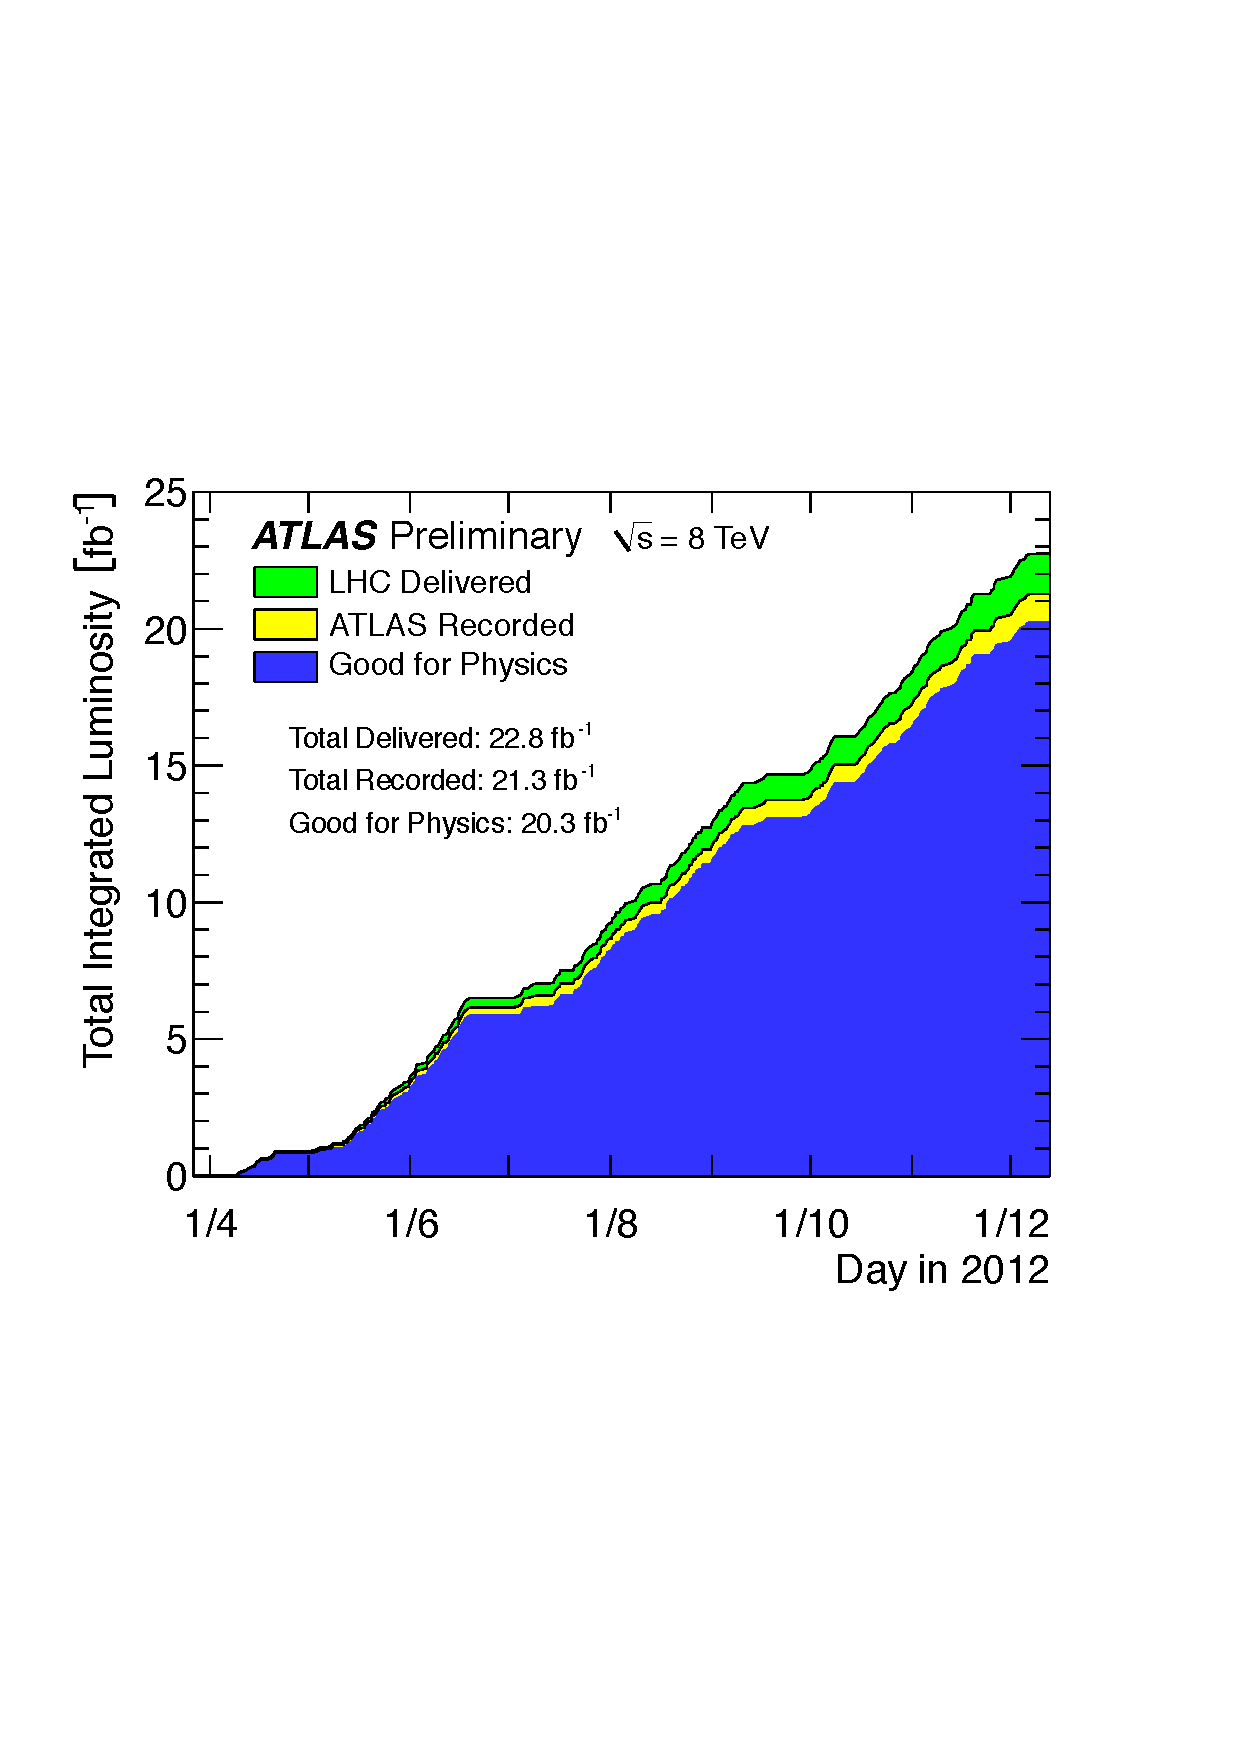
\includegraphics[width=\textwidth]{figures/intlumi}
\end{minipage}\hfill\begin{minipage}[b]{.3\textwidth}
\caption{A plot showing the integrated luminosity delivered by the LHC (green), recorded by ATLAS (yellow), and fulfilling data quality criteria (blue), over the course of the 8 TeV run in 2012 \cite{publiclumi}.
\label{intlumi}}
\end{minipage}
\end{figure}

Unfortunately, the triggers that are implemented in \atlas{} do not guarantee that the event rate remains within the technical limitations of the readout system. To stay within those limits, \atlas{} prescales certian triggers, when they originate from a trigger that produces more events than it is considered worth keeping,\footnote{Explaining how it is decided whether data is worth keeping would veer into a discussion of \atlas{} internal politics, which is a topic beyond the scope of this thesis.} which means simply that a fraction of event that pass a trigger are not recorded. The diphoton channel is important to the search for the Higgs boson, however, so the triggers that produce diphotons events have not been prescaled.


\chapter{Data preparation}

For the present analysis, we will use events that passed the \texttt{2g40\_loose} level--1 trigger, which requires that the EM calorimeter reports two hits with at least 40~GeV of transverse energy that pass the loose selection criteria, described in the previous chapter.

The datasets have been retrieved in the \texttt{NTUP\_PHOTON} format, which is streamlined to contain information relevant to photon analyses, and easily readable by \textsc{root}. The dataset used contains events corresponding to 18.301~fb$^{-1}$ of integrated luminosity.

On each of the prospective photons in this dataset, we impose a series of selection criteria:

\begin{itemize}
\item \textbf{otx and phoCloan cut:} Object quality cuts, which cut out events too close to non-functioning or noisy detector elements, and events taken while the detector was in a non-optimal state.
\item \textbf{ID cut:} Objects that did not pass photon identification, or do not satisfy the loose selection criteria after reconstruction, are eliminated.
\item \textbf{kinematics cut:} Ensures that objects do not have $|\eta|$ greater than 2.37, which is the forward limit of the first layer of the EM calorimeter, or in the range between 1.37 and 1.52, which is the transition region between the barrel and endcap calorimeters. Also ensures $E_T$ greater than 50~GeV, which clears the turn--on curve of the \texttt{2g40\_loose} trigger.
\item \textbf{N\_events cut:} Ensures that each event has at least two photons that pass the above criteria.
%\item \textbf{PV cut:} Ensures that the photon pair selected for analysis have the same primary vertex, and that that vertex has at least three tracks associated with it.

\end{itemize}

The number of objects remaining at each step of the cut procedure is plotted in figure~\ref{cutflow}

\begin{figure}[htp]
\begin{minipage}[b]{.69\textwidth}
\begin{infilsf} \tiny
\begin{tikzpicture}[x=.1\textwidth,y=.1\textwidth]
\pgfdeclareplotmark{cross} {
\pgfpathmoveto{\pgfpoint{-0.3\pgfplotmarksize}{\pgfplotmarksize}}
\pgfpathlineto{\pgfpoint{+0.3\pgfplotmarksize}{\pgfplotmarksize}}
\pgfpathlineto{\pgfpoint{+0.3\pgfplotmarksize}{0.3\pgfplotmarksize}}
\pgfpathlineto{\pgfpoint{+1\pgfplotmarksize}{0.3\pgfplotmarksize}}
\pgfpathlineto{\pgfpoint{+1\pgfplotmarksize}{-0.3\pgfplotmarksize}}
\pgfpathlineto{\pgfpoint{+0.3\pgfplotmarksize}{-0.3\pgfplotmarksize}}
\pgfpathlineto{\pgfpoint{+0.3\pgfplotmarksize}{-1.\pgfplotmarksize}}
\pgfpathlineto{\pgfpoint{-0.3\pgfplotmarksize}{-1.\pgfplotmarksize}}
\pgfpathlineto{\pgfpoint{-0.3\pgfplotmarksize}{-0.3\pgfplotmarksize}}
\pgfpathlineto{\pgfpoint{-1.\pgfplotmarksize}{-0.3\pgfplotmarksize}}
\pgfpathlineto{\pgfpoint{-1.\pgfplotmarksize}{0.3\pgfplotmarksize}}
\pgfpathlineto{\pgfpoint{-0.3\pgfplotmarksize}{0.3\pgfplotmarksize}}
\pgfpathclose
\pgfusepathqstroke
}
\pgfdeclareplotmark{cross*} {
\pgfpathmoveto{\pgfpoint{-0.3\pgfplotmarksize}{\pgfplotmarksize}}
\pgfpathlineto{\pgfpoint{+0.3\pgfplotmarksize}{\pgfplotmarksize}}
\pgfpathlineto{\pgfpoint{+0.3\pgfplotmarksize}{0.3\pgfplotmarksize}}
\pgfpathlineto{\pgfpoint{+1\pgfplotmarksize}{0.3\pgfplotmarksize}}
\pgfpathlineto{\pgfpoint{+1\pgfplotmarksize}{-0.3\pgfplotmarksize}}
\pgfpathlineto{\pgfpoint{+0.3\pgfplotmarksize}{-0.3\pgfplotmarksize}}
\pgfpathlineto{\pgfpoint{+0.3\pgfplotmarksize}{-1.\pgfplotmarksize}}
\pgfpathlineto{\pgfpoint{-0.3\pgfplotmarksize}{-1.\pgfplotmarksize}}
\pgfpathlineto{\pgfpoint{-0.3\pgfplotmarksize}{-0.3\pgfplotmarksize}}
\pgfpathlineto{\pgfpoint{-1.\pgfplotmarksize}{-0.3\pgfplotmarksize}}
\pgfpathlineto{\pgfpoint{-1.\pgfplotmarksize}{0.3\pgfplotmarksize}}
\pgfpathlineto{\pgfpoint{-0.3\pgfplotmarksize}{0.3\pgfplotmarksize}}
\pgfpathclose
\pgfusepathqfillstroke
}
\pgfdeclareplotmark{newstar} {
\pgfpathmoveto{\pgfqpoint{0pt}{\pgfplotmarksize}}
\pgfpathlineto{\pgfqpointpolar{44}{0.5\pgfplotmarksize}}
\pgfpathlineto{\pgfqpointpolar{18}{\pgfplotmarksize}}
\pgfpathlineto{\pgfqpointpolar{-20}{0.5\pgfplotmarksize}}
\pgfpathlineto{\pgfqpointpolar{-54}{\pgfplotmarksize}}
\pgfpathlineto{\pgfqpointpolar{-90}{0.5\pgfplotmarksize}}
\pgfpathlineto{\pgfqpointpolar{234}{\pgfplotmarksize}}
\pgfpathlineto{\pgfqpointpolar{198}{0.5\pgfplotmarksize}}
\pgfpathlineto{\pgfqpointpolar{162}{\pgfplotmarksize}}
\pgfpathlineto{\pgfqpointpolar{134}{0.5\pgfplotmarksize}}
\pgfpathclose
\pgfusepathqstroke
}
\pgfdeclareplotmark{newstar*} {
\pgfpathmoveto{\pgfqpoint{0pt}{\pgfplotmarksize}}
\pgfpathlineto{\pgfqpointpolar{44}{0.5\pgfplotmarksize}}
\pgfpathlineto{\pgfqpointpolar{18}{\pgfplotmarksize}}
\pgfpathlineto{\pgfqpointpolar{-20}{0.5\pgfplotmarksize}}
\pgfpathlineto{\pgfqpointpolar{-54}{\pgfplotmarksize}}
\pgfpathlineto{\pgfqpointpolar{-90}{0.5\pgfplotmarksize}}
\pgfpathlineto{\pgfqpointpolar{234}{\pgfplotmarksize}}
\pgfpathlineto{\pgfqpointpolar{198}{0.5\pgfplotmarksize}}
\pgfpathlineto{\pgfqpointpolar{162}{\pgfplotmarksize}}
\pgfpathlineto{\pgfqpointpolar{134}{0.5\pgfplotmarksize}}
\pgfpathclose
\pgfusepathqfillstroke
}
\definecolor{c}{rgb}{1,1,1};
\draw [color=c, fill=c] (0,0) rectangle (10,6.79598);
\draw [color=c, fill=c] (1,0.679598) rectangle (9,6.11638);
\definecolor{c}{rgb}{0,0,0};
\draw [c] (1,0.679598) -- (1,6.11638) -- (9,6.11638) -- (9,0.679598) -- (1,0.679598);
\definecolor{c}{rgb}{1,1,1};
\draw [color=c, fill=c] (1,0.679598) rectangle (9,6.11638);
\definecolor{c}{rgb}{0,0,0};
\draw [c] (1,0.679598) -- (1,6.11638) -- (9,6.11638) -- (9,0.679598) -- (1,0.679598);
\definecolor{c}{named}{natgreen};
\draw [c] (1.66667,5.85628) -- (1.66667,5.85688);
\draw [c] (1.66667,5.85688) -- (1.66667,5.85748);
\draw [c] (1,5.85688) -- (1.66667,5.85688);
\draw [c] (1.66667,5.85688) -- (2.33333,5.85688);
\definecolor{c}{rgb}{0,0,0};
\definecolor{c}{named}{natgreen};
\draw [c] (3,5.84891) -- (3,5.84951);
\draw [c] (3,5.84951) -- (3,5.85011);
\draw [c] (2.33333,5.84951) -- (3,5.84951);
\draw [c] (3,5.84951) -- (3.66667,5.84951);
\definecolor{c}{rgb}{0,0,0};
\definecolor{c}{named}{natgreen};
\draw [c] (4.33333,5.79306) -- (4.33333,5.79365);
\draw [c] (4.33333,5.79365) -- (4.33333,5.79425);
\draw [c] (3.66667,5.79365) -- (4.33333,5.79365);
\draw [c] (4.33333,5.79365) -- (5,5.79365);
\definecolor{c}{rgb}{0,0,0};
\definecolor{c}{named}{natgreen};
\draw [c] (5.66667,4.055) -- (5.66667,4.05549);
\draw [c] (5.66667,4.05549) -- (5.66667,4.05597);
\draw [c] (5,4.05549) -- (5.66667,4.05549);
\draw [c] (5.66667,4.05549) -- (6.33333,4.05549);
\definecolor{c}{rgb}{0,0,0};
\definecolor{c}{named}{natgreen};
\draw [c] (7,1.19538) -- (7,1.19557);
\draw [c] (7,1.19557) -- (7,1.19576);
\draw [c] (6.33333,1.19557) -- (7,1.19557);
\draw [c] (7,1.19557) -- (7.66667,1.19557);
\definecolor{c}{rgb}{0,0,0};
\definecolor{c}{named}{natgreen};
\draw [c] (8.33333,0.856746) -- (8.33333,0.856825);
\draw [c] (8.33333,0.856825) -- (8.33333,0.856903);
\draw [c] (7.66667,0.856825) -- (8.33333,0.856825);
\draw [c] (8.33333,0.856825) -- (9,0.856825);
\definecolor{c}{rgb}{0,0,0};
\draw [c] (1,0.679598) -- (9,0.679598);
\draw [anchor=north] (1.66667,0.598046) node[color=c, rotate=0]{All};
\draw [anchor=north] (3,0.598046)       node[color=c, rotate=0]{\phantom{H}otx\_cut\phantom{H}};
\draw [anchor=north] (4.33333,0.598046) node[color=c, rotate=0]{phoClean\_cut};
\draw [anchor=north] (5.66667,0.598046) node[color=c, rotate=0]{ID\_cut};
\draw [anchor=north] (7,0.598046)       node[color=c, rotate=0]{kinematics\_cut};
\draw [anchor=north] (8.33333,0.598046) node[color=c, rotate=0]{N\_events};
\draw [c] (1,0.842701) -- (1,0.679598);
\draw [c] (2.33333,0.842701) -- (2.33333,0.679598);
\draw [c] (3.66667,0.842701) -- (3.66667,0.679598);
\draw [c] (5,0.842701) -- (5,0.679598);
\draw [c] (6.33333,0.842701) -- (6.33333,0.679598);
\draw [c] (7.66667,0.842701) -- (7.66667,0.679598);
\draw [c] (9,0.842701) -- (9,0.679598);
\draw [c] (1,0.679598) -- (1,6.11638);
\draw [anchor= east] (0.44,6.11638) node[color=c, rotate=90]{Number of accepted photons};
\draw [c] (1.24,0.679598) -- (1,0.679598);
\draw [c] (1.12,0.818827) -- (1,0.818827);
\draw [c] (1.12,0.958056) -- (1,0.958056);
\draw [c] (1.12,1.09729) -- (1,1.09729);
\draw [c] (1.12,1.23652) -- (1,1.23652);
\draw [c] (1.24,1.37574) -- (1,1.37574);
\draw [c] (1.12,1.51497) -- (1,1.51497);
\draw [c] (1.12,1.6542) -- (1,1.6542);
\draw [c] (1.12,1.79343) -- (1,1.79343);
\draw [c] (1.12,1.93266) -- (1,1.93266);
\draw [c] (1.24,2.07189) -- (1,2.07189);
\draw [c] (1.12,2.21112) -- (1,2.21112);
\draw [c] (1.12,2.35035) -- (1,2.35035);
\draw [c] (1.12,2.48958) -- (1,2.48958);
\draw [c] (1.12,2.62881) -- (1,2.62881);
\draw [c] (1.24,2.76804) -- (1,2.76804);
\draw [c] (1.12,2.90727) -- (1,2.90727);
\draw [c] (1.12,3.0465) -- (1,3.0465);
\draw [c] (1.12,3.18573) -- (1,3.18573);
\draw [c] (1.12,3.32496) -- (1,3.32496);
\draw [c] (1.24,3.46418) -- (1,3.46418);
\draw [c] (1.12,3.60341) -- (1,3.60341);
\draw [c] (1.12,3.74264) -- (1,3.74264);
\draw [c] (1.12,3.88187) -- (1,3.88187);
\draw [c] (1.12,4.0211) -- (1,4.0211);
\draw [c] (1.24,4.16033) -- (1,4.16033);
\draw [c] (1.12,4.29956) -- (1,4.29956);
\draw [c] (1.12,4.43879) -- (1,4.43879);
\draw [c] (1.12,4.57802) -- (1,4.57802);
\draw [c] (1.12,4.71725) -- (1,4.71725);
\draw [c] (1.24,4.85648) -- (1,4.85648);
\draw [c] (1.12,4.99571) -- (1,4.99571);
\draw [c] (1.12,5.13494) -- (1,5.13494);
\draw [c] (1.12,5.27417) -- (1,5.27417);
\draw [c] (1.12,5.4134) -- (1,5.4134);
\draw [c] (1.24,5.55263) -- (1,5.55263);
\draw [c] (1.24,5.55263) -- (1,5.55263);
\draw [c] (1.12,5.69185) -- (1,5.69185);
\draw [c] (1.12,5.83108) -- (1,5.83108);
\draw [c] (1.12,5.97031) -- (1,5.97031);
\draw [c] (1.12,6.10954) -- (1,6.10954);
\draw [anchor= east] (0.95,0.679598) node[color=c, rotate=0]{0};
\draw [anchor= east] (0.95,1.37574) node[color=c, rotate=0]{10};
\draw [anchor= east] (0.95,2.07189) node[color=c, rotate=0]{20};
\draw [anchor= east] (0.95,2.76804) node[color=c, rotate=0]{30};
\draw [anchor= east] (0.95,3.46418) node[color=c, rotate=0]{40};
\draw [anchor= east] (0.95,4.16033) node[color=c, rotate=0]{50};
\draw [anchor= east] (0.95,4.85648) node[color=c, rotate=0]{60};
\draw [anchor= east] (0.95,5.55263) node[color=c, rotate=0]{70};
\draw [anchor=base west] (1,6.14017) node[color=c, rotate=0]{$\times10^{6}$};
\end{tikzpicture}

\end{infilsf}
\end{minipage}\hfill\begin{minipage}[b]{.3\textwidth}
\caption{A cutflow diagram, showing how many objects remain in the dataset after each of the selection criteria are imposed. The final number of photons is (something I sould be able to dig up somewhere).
\label{cutflow}}
\end{minipage}
\end{figure}

What remains after these cuts have been applied is a purer sample of photons than we had before, however the sample will still contain a background of events that do not come from the processes that we wish to study. An estimate of this background is required.

\section{Data driven background estimation}
The background that remains in the signal sample after these criteria have been applied can be estimated in a number of ways. In chapter~\ref{ch.mc}, monte  carlo samples that simulate several physical processes that act as background to diphoton events were presented. Here, however, we shall attempt to quantify the magnitude of the background by examining the data.

\subsection{The ABCD method}
Also known as the two--dimensional sideband method, illustrated in figure~\ref{abcd}.

\begin{figure}[hbp]
  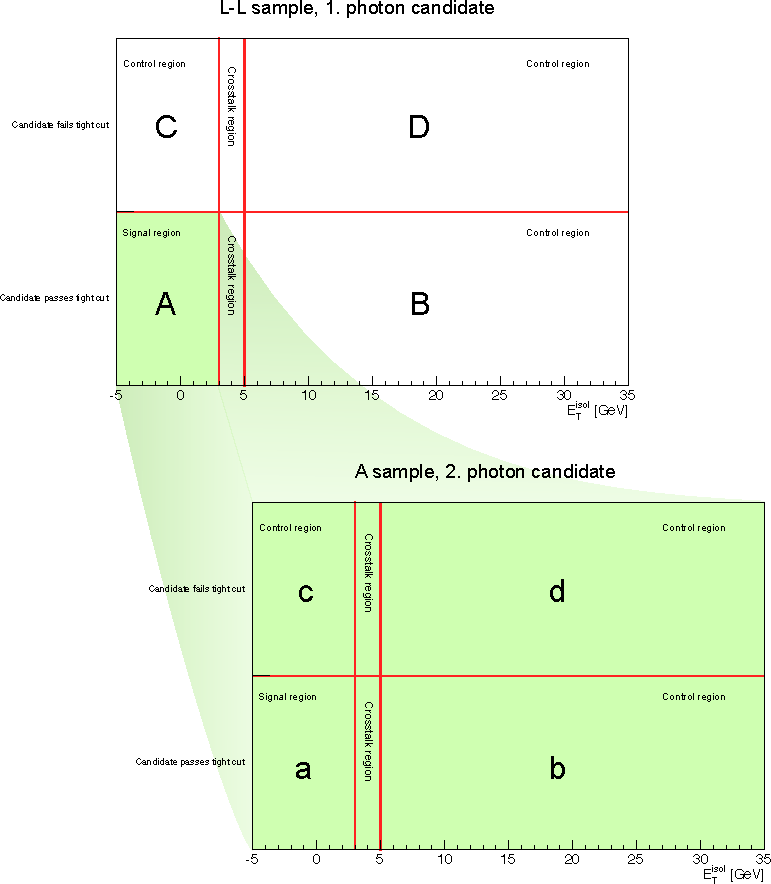
\includegraphics[width=\textwidth]{figures/sideband}
  \caption{Illustrating the two--step ABCD method using the `tight' selection criteria and the isolation energy: the full set of diphotons (the L-L sample) is split into four groups---A, B, C and D---according to the discriminating variables for the leading photon. Signal photons are now confined to the A region. The events in the C region can be used to estimate the shape, and the B and D region can be used to estimate the magnitude of the distribution of background events in the signal region. The procedure is then repeated for the subleading partner photons of the events in the A region. This gives an estimate of the distibution of background events in the combined signal (A--A) region. This figure adapted from \cite{fdirect}.}\label{abcd}
\end{figure}

By taking two uncorrelated discriminating variables, we can split the distribution of one of them into two, according to the other discriminating variable, one sample with pure background events, and the other with signal and background events. Assuming that the shape of the distribution of background events is the same in the mixed signal and background sample as it is in the pure background sample, the shape of the distribution in the signal region of the background sample, this is the C region, is the same as the shape of the distribution of background events in the signal region of the mixed sample, the A region. The B and D regions contain only background events, so the magnitude of the background distribution in the A region can be found by comparing the sidebands. For more detail, see \cite{cmsabcd}

For the diphoton sample, we will use the `tight' selection criteria, which were described in chapter~\ref{ch.ex}, and the transverse isolation energy, $E_T^{\text{isol}}$, the energy deposited in the calorimeter in a cone with radius $R\le0.4$, but outside $R\le0.2$, where
\[R=\sqrt{\Delta\phi^2+\Delta\theta^2}.\]
The signal region is cut at $E_T^{\text{isol}}\le3$ GeV. We allow a crosstalk region of 2 GeV, which means the background region is defined with $5\text{ GeV}\le E_T^{\text{isol}}\le25\text{ GeV}$. The distribution of $E_T^{\text{isol}}$ for leading photons and subleading photons in the `A' sample is given in figure~\ref{etiso}.

\begin{figure}[htp]
\begin{minipage}[b]{.69\textwidth}
\begin{infilsf} \tiny 
\begin{tikzpicture}[x=.1\textwidth,y=.1\textwidth]
\pgfdeclareplotmark{cross} {
\pgfpathmoveto{\pgfpoint{-0.3\pgfplotmarksize}{\pgfplotmarksize}}
\pgfpathlineto{\pgfpoint{+0.3\pgfplotmarksize}{\pgfplotmarksize}}
\pgfpathlineto{\pgfpoint{+0.3\pgfplotmarksize}{0.3\pgfplotmarksize}}
\pgfpathlineto{\pgfpoint{+1\pgfplotmarksize}{0.3\pgfplotmarksize}}
\pgfpathlineto{\pgfpoint{+1\pgfplotmarksize}{-0.3\pgfplotmarksize}}
\pgfpathlineto{\pgfpoint{+0.3\pgfplotmarksize}{-0.3\pgfplotmarksize}}
\pgfpathlineto{\pgfpoint{+0.3\pgfplotmarksize}{-1.\pgfplotmarksize}}
\pgfpathlineto{\pgfpoint{-0.3\pgfplotmarksize}{-1.\pgfplotmarksize}}
\pgfpathlineto{\pgfpoint{-0.3\pgfplotmarksize}{-0.3\pgfplotmarksize}}
\pgfpathlineto{\pgfpoint{-1.\pgfplotmarksize}{-0.3\pgfplotmarksize}}
\pgfpathlineto{\pgfpoint{-1.\pgfplotmarksize}{0.3\pgfplotmarksize}}
\pgfpathlineto{\pgfpoint{-0.3\pgfplotmarksize}{0.3\pgfplotmarksize}}
\pgfpathclose
\pgfusepathqstroke
}
\pgfdeclareplotmark{cross*} {
\pgfpathmoveto{\pgfpoint{-0.3\pgfplotmarksize}{\pgfplotmarksize}}
\pgfpathlineto{\pgfpoint{+0.3\pgfplotmarksize}{\pgfplotmarksize}}
\pgfpathlineto{\pgfpoint{+0.3\pgfplotmarksize}{0.3\pgfplotmarksize}}
\pgfpathlineto{\pgfpoint{+1\pgfplotmarksize}{0.3\pgfplotmarksize}}
\pgfpathlineto{\pgfpoint{+1\pgfplotmarksize}{-0.3\pgfplotmarksize}}
\pgfpathlineto{\pgfpoint{+0.3\pgfplotmarksize}{-0.3\pgfplotmarksize}}
\pgfpathlineto{\pgfpoint{+0.3\pgfplotmarksize}{-1.\pgfplotmarksize}}
\pgfpathlineto{\pgfpoint{-0.3\pgfplotmarksize}{-1.\pgfplotmarksize}}
\pgfpathlineto{\pgfpoint{-0.3\pgfplotmarksize}{-0.3\pgfplotmarksize}}
\pgfpathlineto{\pgfpoint{-1.\pgfplotmarksize}{-0.3\pgfplotmarksize}}
\pgfpathlineto{\pgfpoint{-1.\pgfplotmarksize}{0.3\pgfplotmarksize}}
\pgfpathlineto{\pgfpoint{-0.3\pgfplotmarksize}{0.3\pgfplotmarksize}}
\pgfpathclose
\pgfusepathqfillstroke
}
\pgfdeclareplotmark{newstar} {
\pgfpathmoveto{\pgfqpoint{0pt}{\pgfplotmarksize}}
\pgfpathlineto{\pgfqpointpolar{44}{0.5\pgfplotmarksize}}
\pgfpathlineto{\pgfqpointpolar{18}{\pgfplotmarksize}}
\pgfpathlineto{\pgfqpointpolar{-20}{0.5\pgfplotmarksize}}
\pgfpathlineto{\pgfqpointpolar{-54}{\pgfplotmarksize}}
\pgfpathlineto{\pgfqpointpolar{-90}{0.5\pgfplotmarksize}}
\pgfpathlineto{\pgfqpointpolar{234}{\pgfplotmarksize}}
\pgfpathlineto{\pgfqpointpolar{198}{0.5\pgfplotmarksize}}
\pgfpathlineto{\pgfqpointpolar{162}{\pgfplotmarksize}}
\pgfpathlineto{\pgfqpointpolar{134}{0.5\pgfplotmarksize}}
\pgfpathclose
\pgfusepathqstroke
}
\pgfdeclareplotmark{newstar*} {
\pgfpathmoveto{\pgfqpoint{0pt}{\pgfplotmarksize}}
\pgfpathlineto{\pgfqpointpolar{44}{0.5\pgfplotmarksize}}
\pgfpathlineto{\pgfqpointpolar{18}{\pgfplotmarksize}}
\pgfpathlineto{\pgfqpointpolar{-20}{0.5\pgfplotmarksize}}
\pgfpathlineto{\pgfqpointpolar{-54}{\pgfplotmarksize}}
\pgfpathlineto{\pgfqpointpolar{-90}{0.5\pgfplotmarksize}}
\pgfpathlineto{\pgfqpointpolar{234}{\pgfplotmarksize}}
\pgfpathlineto{\pgfqpointpolar{198}{0.5\pgfplotmarksize}}
\pgfpathlineto{\pgfqpointpolar{162}{\pgfplotmarksize}}
\pgfpathlineto{\pgfqpointpolar{134}{0.5\pgfplotmarksize}}
\pgfpathclose
\pgfusepathqfillstroke
}
\definecolor{c}{rgb}{1,1,1};
\draw [color=c, fill=c] (1,0.679598) rectangle (9,6.11638);
\definecolor{c}{rgb}{0,0,0};
\draw [c] (1,0.679598) -- (1,6.11638) -- (9,6.11638) -- (9,0.679598) -- (1,0.679598);
\definecolor{c}{rgb}{1,1,1};
\draw [color=c, fill=c] (1,0.679598) rectangle (9,6.11638);
\definecolor{c}{rgb}{0,0,0};
\draw [c] (1,0.679598) -- (1,6.11638) -- (9,6.11638) -- (9,0.679598) -- (1,0.679598);
\colorlet{c}{natgreen}
\draw [c] (1,0.680318) -- (1.0293,0.680318) -- (1.0293,0.681757) -- (1.05861,0.681757) -- (1.05861,0.681757) -- (1.08791,0.681757) -- (1.08791,0.683197) -- (1.11722,0.683197) -- (1.11722,0.682837) -- (1.14652,0.682837) -- (1.14652,0.682837) --
 (1.17582,0.682837) -- (1.17582,0.684637) -- (1.20513,0.684637) -- (1.20513,0.686437) -- (1.23443,0.686437) -- (1.23443,0.689676) -- (1.26374,0.689676) -- (1.26374,0.691476) -- (1.29304,0.691476) -- (1.29304,0.692916) -- (1.32234,0.692916) --
 (1.32234,0.700115) -- (1.35165,0.700115) -- (1.35165,0.706594) -- (1.38095,0.706594) -- (1.38095,0.718832) -- (1.41026,0.718832) -- (1.41026,0.730711) -- (1.43956,0.730711) -- (1.43956,0.73251) -- (1.46886,0.73251) -- (1.46886,0.749428) --
 (1.49817,0.749428) -- (1.49817,0.765986) -- (1.52747,0.765986) -- (1.52747,0.803421) -- (1.55678,0.803421) -- (1.55678,0.825378) -- (1.58608,0.825378) -- (1.58608,0.872891) -- (1.61538,0.872891) -- (1.61538,0.916085) -- (1.64469,0.916085) --
 (1.64469,0.980156) -- (1.67399,0.980156) -- (1.67399,1.02983) -- (1.7033,1.02983) -- (1.7033,1.13098) -- (1.7326,1.13098) -- (1.7326,1.24976) -- (1.7619,1.24976) -- (1.7619,1.36998) -- (1.79121,1.36998) -- (1.79121,1.47797) -- (1.82051,1.47797) --
 (1.82051,1.70258) -- (1.84982,1.70258) -- (1.84982,1.88471) -- (1.87912,1.88471) -- (1.87912,2.13668) -- (1.90842,2.13668) -- (1.90842,2.44264) -- (1.93773,2.44264) -- (1.93773,2.74931) -- (1.96703,2.74931) -- (1.96703,3.11538) -- (1.99634,3.11538)
 -- (1.99634,3.51025) -- (2.02564,3.51025) -- (2.02564,3.91339) -- (2.05494,3.91339) -- (2.05494,4.39969) -- (2.08425,4.39969) -- (2.08425,4.83019) -- (2.11355,4.83019) -- (2.11355,5.25133) -- (2.14286,5.25133) -- (2.14286,5.5742) -- (2.17216,5.5742)
 -- (2.17216,5.74302) -- (2.20147,5.74302) -- (2.20147,5.85748) -- (2.23077,5.85748) -- (2.23077,5.71314) -- (2.26007,5.71314) -- (2.26007,5.43346) -- (2.28938,5.43346) -- (2.28938,5.30064) -- (2.31868,5.30064) -- (2.31868,5.13362) --
 (2.34799,5.13362) -- (2.34799,4.86654) -- (2.37729,4.86654) -- (2.37729,4.65165) -- (2.40659,4.65165) -- (2.40659,4.41552) -- (2.4359,4.41552) -- (2.4359,4.16608) -- (2.4652,4.16608) -- (2.4652,4.03974) -- (2.49451,4.03974) -- (2.49451,3.90655) --
 (2.52381,3.90655) -- (2.52381,3.68158) -- (2.55311,3.68158) -- (2.55311,3.57216) -- (2.58242,3.57216) -- (2.58242,3.35511) -- (2.61172,3.35511) -- (2.61172,3.31767) -- (2.64103,3.31767) -- (2.64103,3.12546) -- (2.67033,3.12546) -- (2.67033,2.98292)
 -- (2.69963,2.98292) -- (2.69963,2.8429) -- (2.72894,2.8429) -- (2.72894,2.79683) -- (2.75824,2.79683) -- (2.75824,2.59309) -- (2.78755,2.59309) -- (2.78755,2.60389) -- (2.81685,2.60389) -- (2.81685,2.42572) -- (2.84615,2.42572) -- (2.84615,2.37208)
 -- (2.87546,2.37208) -- (2.87546,2.2821) -- (2.90476,2.2821) -- (2.90476,2.19823) -- (2.93407,2.19823) -- (2.93407,2.105) -- (2.96337,2.105) -- (2.96337,2.07477) -- (2.99267,2.07477) -- (2.99267,1.9513) -- (3.02198,1.9513) -- (3.02198,1.91567) --
 (3.05128,1.91567) -- (3.05128,1.8552) -- (3.08059,1.8552) -- (3.08059,1.80192) -- (3.10989,1.80192) -- (3.10989,1.72813) -- (3.13919,1.72813) -- (3.13919,1.70582) -- (3.1685,1.70582) -- (3.1685,1.66298) -- (3.1978,1.66298) -- (3.1978,1.60575) --
 (3.22711,1.60575) -- (3.22711,1.58127) -- (3.25641,1.58127) -- (3.25641,1.53772) -- (3.28571,1.53772) -- (3.28571,1.48373) -- (3.31502,1.48373) -- (3.31502,1.43441) -- (3.34432,1.43441) -- (3.34432,1.44557) -- (3.37363,1.44557) -- (3.37363,1.37754)
 -- (3.40293,1.37754) -- (3.40293,1.35594) -- (3.43223,1.35594) -- (3.43223,1.32931) -- (3.46154,1.32931) -- (3.46154,1.29151) -- (3.49084,1.29151) -- (3.49084,1.30159) -- (3.52015,1.30159) -- (3.52015,1.23608) -- (3.54945,1.23608) --
 (3.54945,1.2476) -- (3.57875,1.2476) -- (3.57875,1.20405) -- (3.60806,1.20405) -- (3.60806,1.19361) -- (3.63736,1.19361) -- (3.63736,1.19181) -- (3.66667,1.19181) -- (3.66667,1.18497) -- (3.69597,1.18497) -- (3.69597,1.14357) -- (3.72527,1.14357) --
 (3.72527,1.11766) -- (3.75458,1.11766) -- (3.75458,1.10074) -- (3.78388,1.10074) -- (3.78388,1.0705) -- (3.81319,1.0705) -- (3.81319,1.08454) -- (3.84249,1.08454) -- (3.84249,1.04675) -- (3.87179,1.04675) -- (3.87179,1.03523) -- (3.9011,1.03523) --
 (3.9011,1.01651) -- (3.9304,1.01651) -- (3.9304,1.01939) -- (3.95971,1.01939) -- (3.95971,1.01039) -- (3.98901,1.01039) -- (3.98901,1.01363) -- (4.01831,1.01363) -- (4.01831,0.979796) -- (4.04762,0.979796) -- (4.04762,0.969358) -- (4.07692,0.969358)
 -- (4.07692,0.944881) -- (4.10623,0.944881) -- (4.10623,0.95316) -- (4.13553,0.95316) -- (4.13553,0.927604) -- (4.16483,0.927604) -- (4.16483,0.927244) -- (4.19414,0.927244) -- (4.19414,0.899168) -- (4.22344,0.899168) -- (4.22344,0.907446) --
 (4.25275,0.907446) -- (4.25275,0.914285) -- (4.28205,0.914285) -- (4.28205,0.890529) -- (4.31136,0.890529) -- (4.31136,0.901687) -- (4.34066,0.901687) -- (4.34066,0.898088) -- (4.36996,0.898088) -- (4.36996,0.88369) -- (4.39927,0.88369) --
 (4.39927,0.87793) -- (4.42857,0.87793) -- (4.42857,0.867852) -- (4.45788,0.867852) -- (4.45788,0.859573) -- (4.48718,0.859573) -- (4.48718,0.850574) -- (4.51648,0.850574) -- (4.51648,0.849854) -- (4.54579,0.849854) -- (4.54579,0.854174) --
 (4.57509,0.854174) -- (4.57509,0.852014) -- (4.6044,0.852014) -- (4.6044,0.847695) -- (4.6337,0.847695) -- (4.6337,0.823578) -- (4.663,0.823578) -- (4.663,0.833297) -- (4.69231,0.833297) -- (4.69231,0.818539) -- (4.72161,0.818539) --
 (4.72161,0.802701) -- (4.75092,0.802701) -- (4.75092,0.818539) -- (4.78022,0.818539) -- (4.78022,0.813499) -- (4.80952,0.813499) -- (4.80952,0.81134) -- (4.83883,0.81134) -- (4.83883,0.799101) -- (4.86813,0.799101) -- (4.86813,0.789743) --
 (4.89744,0.789743) -- (4.89744,0.796942) -- (4.92674,0.796942) -- (4.92674,0.792262) -- (4.95604,0.792262) -- (4.95604,0.795502) -- (4.98535,0.795502) -- (4.98535,0.797661) -- (5.01465,0.797661) -- (5.01465,0.777144) -- (5.04396,0.777144) --
 (5.04396,0.783983) -- (5.07326,0.783983) -- (5.07326,0.776784) -- (5.10256,0.776784) -- (5.10256,0.770305) -- (5.13187,0.770305) -- (5.13187,0.773545) -- (5.16117,0.773545) -- (5.16117,0.778584) -- (5.19048,0.778584) -- (5.19048,0.772465) --
 (5.21978,0.772465) -- (5.21978,0.764186) -- (5.24908,0.764186) -- (5.24908,0.763106) -- (5.27839,0.763106) -- (5.27839,0.760227) -- (5.30769,0.760227) -- (5.30769,0.762026) -- (5.337,0.762026) -- (5.337,0.756627) -- (5.3663,0.756627) --
 (5.3663,0.762746) -- (5.3956,0.762746) -- (5.3956,0.757707) -- (5.42491,0.757707) -- (5.42491,0.755187) -- (5.45421,0.755187) -- (5.45421,0.747628) -- (5.48352,0.747628) -- (5.48352,0.745469) -- (5.51282,0.745469) -- (5.51282,0.747268) --
 (5.54212,0.747268) -- (5.54212,0.753388) -- (5.57143,0.753388) -- (5.57143,0.746908) -- (5.60073,0.746908) -- (5.60073,0.73827) -- (5.63004,0.73827) -- (5.63004,0.741869) -- (5.65934,0.741869) -- (5.65934,0.742229) -- (5.68864,0.742229) --
 (5.68864,0.739709) -- (5.71795,0.739709) -- (5.71795,0.73863) -- (5.74725,0.73863) -- (5.74725,0.731431) -- (5.77656,0.731431) -- (5.77656,0.728551) -- (5.80586,0.728551) -- (5.80586,0.731431) -- (5.83517,0.731431) -- (5.83517,0.731791) --
 (5.86447,0.731791) -- (5.86447,0.730351) -- (5.89377,0.730351) -- (5.89377,0.725671) -- (5.92308,0.725671) -- (5.92308,0.73935) -- (5.95238,0.73935) -- (5.95238,0.731791) -- (5.98169,0.731791) -- (5.98169,0.727111) -- (6.01099,0.727111) --
 (6.01099,0.728551) -- (6.04029,0.728551) -- (6.04029,0.73467) -- (6.0696,0.73467) -- (6.0696,0.723152) -- (6.0989,0.723152) -- (6.0989,0.728191) -- (6.12821,0.728191) -- (6.12821,0.722792) -- (6.15751,0.722792) -- (6.15751,0.726391) --
 (6.18681,0.726391) -- (6.18681,0.720632) -- (6.21612,0.720632) -- (6.21612,0.717033) -- (6.24542,0.717033) -- (6.24542,0.722432) -- (6.27473,0.722432) -- (6.27473,0.715593) -- (6.30403,0.715593) -- (6.30403,0.719552) -- (6.33333,0.719552) --
 (6.33333,0.717753) -- (6.36264,0.717753) -- (6.36264,0.717393) -- (6.39194,0.717393) -- (6.39194,0.714153) -- (6.42125,0.714153) -- (6.42125,0.716673) -- (6.45055,0.716673) -- (6.45055,0.713433) -- (6.47985,0.713433) -- (6.47985,0.719192) --
 (6.50916,0.719192) -- (6.50916,0.712353) -- (6.53846,0.712353) -- (6.53846,0.713793) -- (6.56777,0.713793) -- (6.56777,0.715593) -- (6.59707,0.715593) -- (6.59707,0.710194) -- (6.62637,0.710194) -- (6.62637,0.718832) -- (6.65568,0.718832) --
 (6.65568,0.713793) -- (6.68498,0.713793) -- (6.68498,0.706954) -- (6.71429,0.706954) -- (6.71429,0.715593) -- (6.74359,0.715593) -- (6.74359,0.708394) -- (6.77289,0.708394) -- (6.77289,0.711633) -- (6.8022,0.711633) -- (6.8022,0.708394) --
 (6.8315,0.708394) -- (6.8315,0.705154) -- (6.86081,0.705154) -- (6.86081,0.707314) -- (6.89011,0.707314) -- (6.89011,0.711633) -- (6.91941,0.711633) -- (6.91941,0.709834) -- (6.94872,0.709834) -- (6.94872,0.707314) -- (6.97802,0.707314) --
 (6.97802,0.707314) -- (7.00733,0.707314) -- (7.00733,0.704434) -- (7.03663,0.704434) -- (7.03663,0.707314) -- (7.06593,0.707314) -- (7.06593,0.706954) -- (7.09524,0.706954) -- (7.09524,0.703354) -- (7.12454,0.703354) -- (7.12454,0.704794) --
 (7.15385,0.704794) -- (7.15385,0.708754) -- (7.18315,0.708754) -- (7.18315,0.703714) -- (7.21245,0.703714) -- (7.21245,0.709834) -- (7.24176,0.709834) -- (7.24176,0.699755) -- (7.27106,0.699755) -- (7.27106,0.702275) -- (7.30037,0.702275) --
 (7.30037,0.704074) -- (7.32967,0.704074) -- (7.32967,0.700835) -- (7.35897,0.700835) -- (7.35897,0.703354) -- (7.38828,0.703354) -- (7.38828,0.705514) -- (7.41758,0.705514) -- (7.41758,0.696155) -- (7.44689,0.696155) -- (7.44689,0.697595) --
 (7.47619,0.697595) -- (7.47619,0.708034) -- (7.50549,0.708034) -- (7.50549,0.700835) -- (7.5348,0.700835) -- (7.5348,0.700115) -- (7.5641,0.700115) -- (7.5641,0.698315) -- (7.59341,0.698315) -- (7.59341,0.697955) -- (7.62271,0.697955) --
 (7.62271,0.700835) -- (7.65201,0.700835) -- (7.65201,0.702635) -- (7.68132,0.702635) -- (7.68132,0.694716) -- (7.71062,0.694716) -- (7.71062,0.698315) -- (7.73993,0.698315) -- (7.73993,0.703354) -- (7.76923,0.703354) -- (7.76923,0.694716) --
 (7.79853,0.694716) -- (7.79853,0.699035) -- (7.82784,0.699035) -- (7.82784,0.697955) -- (7.85714,0.697955) -- (7.85714,0.697955) -- (7.88645,0.697955) -- (7.88645,0.699755) -- (7.91575,0.699755) -- (7.91575,0.701195) -- (7.94506,0.701195) --
 (7.94506,0.699755) -- (7.97436,0.699755) -- (7.97436,0.694356) -- (8.00366,0.694356) -- (8.00366,0.697955) -- (8.03297,0.697955) -- (8.03297,0.696515) -- (8.06227,0.696515) -- (8.06227,0.697595) -- (8.09157,0.697595) -- (8.09157,0.694356) --
 (8.12088,0.694356) -- (8.12088,0.699395) -- (8.15018,0.699395) -- (8.15018,0.695076) -- (8.17949,0.695076) -- (8.17949,0.695796) -- (8.20879,0.695796) -- (8.20879,0.695436) -- (8.2381,0.695436) -- (8.2381,0.697235) -- (8.2674,0.697235) --
 (8.2674,0.694716) -- (8.2967,0.694716) -- (8.2967,0.694356) -- (8.32601,0.694356) -- (8.32601,0.692556) -- (8.35531,0.692556) -- (8.35531,0.692196) -- (8.38461,0.692196) -- (8.38461,0.695076) -- (8.41392,0.695076) -- (8.41392,0.697235) --
 (8.44322,0.697235) -- (8.44322,0.694716) -- (8.47253,0.694716) -- (8.47253,0.696155) -- (8.50183,0.696155) -- (8.50183,0.694716) -- (8.53114,0.694716) -- (8.53114,0.696155) -- (8.56044,0.696155) -- (8.56044,0.692916) -- (8.58974,0.692916) --
 (8.58974,0.693276) -- (8.61905,0.693276) -- (8.61905,0.688596) -- (8.64835,0.688596) -- (8.64835,0.691476) -- (8.67766,0.691476) -- (8.67766,0.690756) -- (8.70696,0.690756) -- (8.70696,0.688956) -- (8.73626,0.688956) -- (8.73626,0.691476) --
 (8.76557,0.691476) -- (8.76557,0.691476) -- (8.79487,0.691476) -- (8.79487,0.695796) -- (8.82418,0.695796) -- (8.82418,0.692556) -- (8.85348,0.692556) -- (8.85348,0.692556) -- (8.88278,0.692556) -- (8.88278,0.693996) -- (8.91209,0.693996) --
 (8.91209,0.695076) -- (8.94139,0.695076) -- (8.94139,0.689676) -- (8.9707,0.689676) -- (8.9707,0.691116) -- (9,0.691116);
\definecolor{c}{rgb}{0,0,0};
\draw [c] (1,0.679598) -- (9,0.679598);
\draw [anchor= east] (9,0.299023) node[color=c, rotate=0]{$E_{T}^{\text{isol}}$ [GeV]};
\draw [c] (1,0.842701) -- (1,0.679598);
\draw [c] (1.2664,0.761149) -- (1.2664,0.679598);
\draw [c] (1.5328,0.761149) -- (1.5328,0.679598);
\draw [c] (1.7992,0.761149) -- (1.7992,0.679598);
\draw [c] (2.0656,0.761149) -- (2.0656,0.679598);
\draw [c] (2.332,0.842701) -- (2.332,0.679598);
\draw [c] (2.5984,0.761149) -- (2.5984,0.679598);
\draw [c] (2.8648,0.761149) -- (2.8648,0.679598);
\draw [c] (3.1312,0.761149) -- (3.1312,0.679598);
\draw [c] (3.3976,0.761149) -- (3.3976,0.679598);
\draw [c] (3.664,0.842701) -- (3.664,0.679598);
\draw [c] (3.9304,0.761149) -- (3.9304,0.679598);
\draw [c] (4.1968,0.761149) -- (4.1968,0.679598);
\draw [c] (4.4632,0.761149) -- (4.4632,0.679598);
\draw [c] (4.7296,0.761149) -- (4.7296,0.679598);
\draw [c] (4.996,0.842701) -- (4.996,0.679598);
\draw [c] (5.2624,0.761149) -- (5.2624,0.679598);
\draw [c] (5.5288,0.761149) -- (5.5288,0.679598);
\draw [c] (5.7952,0.761149) -- (5.7952,0.679598);
\draw [c] (6.0616,0.761149) -- (6.0616,0.679598);
\draw [c] (6.32801,0.842701) -- (6.32801,0.679598);
\draw [c] (6.59441,0.761149) -- (6.59441,0.679598);
\draw [c] (6.86081,0.761149) -- (6.86081,0.679598);
\draw [c] (7.12721,0.761149) -- (7.12721,0.679598);
\draw [c] (7.39361,0.761149) -- (7.39361,0.679598);
\draw [c] (7.66001,0.842701) -- (7.66001,0.679598);
\draw [c] (7.92641,0.761149) -- (7.92641,0.679598);
\draw [c] (8.19281,0.761149) -- (8.19281,0.679598);
\draw [c] (8.45921,0.761149) -- (8.45921,0.679598);
\draw [c] (8.72561,0.761149) -- (8.72561,0.679598);
\draw [c] (8.99201,0.842701) -- (8.99201,0.679598);
\draw [c] (8.99201,0.842701) -- (8.99201,0.679598);
\draw [anchor=base] (1,0.455331) node[color=c, rotate=0]{-5};
\draw [anchor=base] (2.332,0.455331) node[color=c, rotate=0]{0};
\draw [anchor=base] (3.664,0.455331) node[color=c, rotate=0]{5};
\draw [anchor=base] (4.996,0.455331) node[color=c, rotate=0]{10};
\draw [anchor=base] (6.32801,0.455331) node[color=c, rotate=0]{15};
\draw [anchor=base] (7.66001,0.455331) node[color=c, rotate=0]{20};
\draw [anchor=base] (8.99201,0.455331) node[color=c, rotate=0]{25};
\draw [c] (1,0.679598) -- (1,6.11638);
\draw [anchor= east] (0.0,6.11638) node[color=c, rotate=90]{Number of events};
\draw [c] (1.24,0.679598) -- (1,0.679598);
\draw [c] (1.12,0.859573) -- (1,0.859573);
\draw [c] (1.12,1.03955) -- (1,1.03955);
\draw [c] (1.12,1.21952) -- (1,1.21952);
\draw [c] (1.24,1.3995) -- (1,1.3995);
\draw [c] (1.12,1.57947) -- (1,1.57947);
\draw [c] (1.12,1.75945) -- (1,1.75945);
\draw [c] (1.12,1.93942) -- (1,1.93942);
\draw [c] (1.24,2.1194) -- (1,2.1194);
\draw [c] (1.12,2.29937) -- (1,2.29937);
\draw [c] (1.12,2.47935) -- (1,2.47935);
\draw [c] (1.12,2.65933) -- (1,2.65933);
\draw [c] (1.24,2.8393) -- (1,2.8393);
\draw [c] (1.12,3.01928) -- (1,3.01928);
\draw [c] (1.12,3.19925) -- (1,3.19925);
\draw [c] (1.12,3.37923) -- (1,3.37923);
\draw [c] (1.24,3.5592) -- (1,3.5592);
\draw [c] (1.12,3.73918) -- (1,3.73918);
\draw [c] (1.12,3.91915) -- (1,3.91915);
\draw [c] (1.12,4.09913) -- (1,4.09913);
\draw [c] (1.24,4.2791) -- (1,4.2791);
\draw [c] (1.12,4.45908) -- (1,4.45908);
\draw [c] (1.12,4.63905) -- (1,4.63905);
\draw [c] (1.12,4.81903) -- (1,4.81903);
\draw [c] (1.24,4.999) -- (1,4.999);
\draw [c] (1.12,5.17898) -- (1,5.17898);
\draw [c] (1.12,5.35895) -- (1,5.35895);
\draw [c] (1.12,5.53893) -- (1,5.53893);
\draw [c] (1.24,5.7189) -- (1,5.7189);
\draw [c] (1.24,5.7189) -- (1,5.7189);
\draw [c] (1.12,5.89888) -- (1,5.89888);
\draw [c] (1.12,6.07885) -- (1,6.07885);
\draw [anchor= east] (0.95,0.679598) node[color=c, rotate=0]{0};
\draw [anchor= east] (0.95,1.3995) node[color=c, rotate=0]{2000};
\draw [anchor= east] (0.95,2.1194) node[color=c, rotate=0]{4000};
\draw [anchor= east] (0.95,2.8393) node[color=c, rotate=0]{6000};
\draw [anchor= east] (0.95,3.5592) node[color=c, rotate=0]{8000};
\draw [anchor= east] (0.95,4.2791) node[color=c, rotate=0]{10000};
\draw [anchor= east] (0.95,4.999) node[color=c, rotate=0]{12000};
\draw [anchor= east] (0.95,5.7189) node[color=c, rotate=0]{14000};
\colorlet{c}{natgreen!50}
\draw [c] (1,0.679598) -- (1.0293,0.679598) -- (1.0293,0.679598) -- (1.05861,0.679598) -- (1.05861,0.679598) -- (1.08791,0.679598) -- (1.08791,0.679598) -- (1.11722,0.679598) -- (1.11722,0.679598) -- (1.14652,0.679598) -- (1.14652,0.679598) --
 (1.17582,0.679598) -- (1.17582,0.679598) -- (1.20513,0.679598) -- (1.20513,0.680546) -- (1.23443,0.680546) -- (1.23443,0.680546) -- (1.26374,0.680546) -- (1.26374,0.681359) -- (1.29304,0.681359) -- (1.29304,0.682307) -- (1.32234,0.682307) --
 (1.32234,0.683526) -- (1.35165,0.683526) -- (1.35165,0.684745) -- (1.38095,0.684745) -- (1.38095,0.683932) -- (1.41026,0.683932) -- (1.41026,0.684339) -- (1.43956,0.684339) -- (1.43956,0.688267) -- (1.46886,0.688267) -- (1.46886,0.688809) --
 (1.49817,0.688809) -- (1.49817,0.694227) -- (1.52747,0.694227) -- (1.52747,0.694633) -- (1.55678,0.694633) -- (1.55678,0.700457) -- (1.58608,0.700457) -- (1.58608,0.707366) -- (1.61538,0.707366) -- (1.61538,0.715899) -- (1.64469,0.715899) --
 (1.64469,0.72362) -- (1.67399,0.72362) -- (1.67399,0.733643) -- (1.7033,0.733643) -- (1.7033,0.745834) -- (1.7326,0.745834) -- (1.7326,0.760327) -- (1.7619,0.760327) -- (1.7619,0.777665) -- (1.79121,0.777665) -- (1.79121,0.800963) --
 (1.82051,0.800963) -- (1.82051,0.835368) -- (1.84982,0.835368) -- (1.84982,0.859885) -- (1.87912,0.859885) -- (1.87912,0.894425) -- (1.90842,0.894425) -- (1.90842,0.9333) -- (1.93773,0.9333) -- (1.93773,0.997098) -- (1.96703,0.997098) --
 (1.96703,1.04207) -- (1.99634,1.04207) -- (1.99634,1.10776) -- (2.02564,1.10776) -- (2.02564,1.17413) -- (2.05494,1.17413) -- (2.05494,1.23211) -- (2.08425,1.23211) -- (2.08425,1.31907) -- (2.11355,1.31907) -- (2.11355,1.41091) -- (2.14286,1.41091)
 -- (2.14286,1.46563) -- (2.17216,1.46563) -- (2.17216,1.54798) -- (2.20147,1.54798) -- (2.20147,1.60487) -- (2.23077,1.60487) -- (2.23077,1.64267) -- (2.26007,1.64267) -- (2.26007,1.69346) -- (2.28938,1.69346) -- (2.28938,1.7471) -- (2.31868,1.7471)
 -- (2.31868,1.76268) -- (2.34799,1.76268) -- (2.34799,1.76769) -- (2.37729,1.76769) -- (2.37729,1.81401) -- (2.40659,1.81401) -- (2.40659,1.84151) -- (2.4359,1.84151) -- (2.4359,1.82675) -- (2.4652,1.82675) -- (2.4652,1.85478) -- (2.49451,1.85478)
 -- (2.49451,1.8407) -- (2.52381,1.8407) -- (2.52381,1.83988) -- (2.55311,1.83988) -- (2.55311,1.82796) -- (2.58242,1.82796) -- (2.58242,1.85668) -- (2.61172,1.85668) -- (2.61172,1.84584) -- (2.64103,1.84584) -- (2.64103,1.82295) -- (2.67033,1.82295)
 -- (2.67033,1.79099) -- (2.69963,1.79099) -- (2.69963,1.79884) -- (2.72894,1.79884) -- (2.72894,1.78286) -- (2.75824,1.78286) -- (2.75824,1.75401) -- (2.78755,1.75401) -- (2.78755,1.75645) -- (2.81685,1.75645) -- (2.81685,1.73829) --
 (2.84615,1.73829) -- (2.84615,1.70877) -- (2.87546,1.70877) -- (2.87546,1.67368) -- (2.90476,1.67368) -- (2.90476,1.6745) -- (2.93407,1.6745) -- (2.93407,1.65161) -- (2.96337,1.65161) -- (2.96337,1.62763) -- (2.99267,1.62763) -- (2.99267,1.60691) --
 (3.02198,1.60691) -- (3.02198,1.59566) -- (3.05128,1.59566) -- (3.05128,1.55841) -- (3.08059,1.55841) -- (3.08059,1.53782) -- (3.10989,1.53782) -- (3.10989,1.51981) -- (3.13919,1.51981) -- (3.13919,1.47863) -- (3.1685,1.47863) -- (3.1685,1.47863) --
 (3.1978,1.47863) -- (3.1978,1.45764) -- (3.22711,1.45764) -- (3.22711,1.43163) -- (3.25641,1.43163) -- (3.25641,1.40197) -- (3.28571,1.40197) -- (3.28571,1.38693) -- (3.31502,1.38693) -- (3.31502,1.36648) -- (3.34432,1.36648) -- (3.34432,1.33844) --
 (3.37363,1.33844) -- (3.37363,1.32665) -- (3.40293,1.32665) -- (3.40293,1.30078) -- (3.43223,1.30078) -- (3.43223,1.28575) -- (3.46154,1.28575) -- (3.46154,1.27545) -- (3.49084,1.27545) -- (3.49084,1.22601) -- (3.52015,1.22601) -- (3.52015,1.22452)
 -- (3.54945,1.22452) -- (3.54945,1.21003) -- (3.57875,1.21003) -- (3.57875,1.19256) -- (3.60806,1.19256) -- (3.60806,1.18158) -- (3.63736,1.18158) -- (3.63736,1.14285) -- (3.66667,1.14285) -- (3.66667,1.14027) -- (3.69597,1.14027) --
 (3.69597,1.13011) -- (3.72527,1.13011) -- (3.72527,1.11819) -- (3.75458,1.11819) -- (3.75458,1.08243) -- (3.78388,1.08243) -- (3.78388,1.08487) -- (3.81319,1.08487) -- (3.81319,1.07525) -- (3.84249,1.07525) -- (3.84249,1.06225) -- (3.87179,1.06225)
 -- (3.87179,1.05914) -- (3.9011,1.05914) -- (3.9011,1.0315) -- (3.9304,1.0315) -- (3.9304,1.0376) -- (3.95971,1.0376) -- (3.95971,1.01985) -- (3.98901,1.01985) -- (3.98901,1.01037) -- (4.01831,1.01037) -- (4.01831,0.988565) -- (4.04762,0.988565) --
 (4.04762,0.991139) -- (4.07692,0.991139) -- (4.07692,0.977458) -- (4.10623,0.977458) -- (4.10623,0.954295) -- (4.13553,0.954295) -- (4.13553,0.941292) -- (4.16483,0.941292) -- (4.16483,0.93926) -- (4.19414,0.93926) -- (4.19414,0.940886) --
 (4.22344,0.940886) -- (4.22344,0.919078) -- (4.25275,0.919078) -- (4.25275,0.91068) -- (4.28205,0.91068) -- (4.28205,0.893613) -- (4.31136,0.893613) -- (4.31136,0.911763) -- (4.34066,0.911763) -- (4.34066,0.899031) -- (4.36996,0.899031) --
 (4.36996,0.890633) -- (4.39927,0.890633) -- (4.39927,0.878713) -- (4.42857,0.878713) -- (4.42857,0.881016) -- (4.45788,0.881016) -- (4.45788,0.874243) -- (4.48718,0.874243) -- (4.48718,0.863949) -- (4.51648,0.863949) -- (4.51648,0.865845) --
 (4.54579,0.865845) -- (4.54579,0.850403) -- (4.57509,0.850403) -- (4.57509,0.845933) -- (4.6044,0.845933) -- (4.6044,0.84187) -- (4.6337,0.84187) -- (4.6337,0.842683) -- (4.663,0.842683) -- (4.663,0.837671) -- (4.69231,0.837671) --
 (4.69231,0.831711) -- (4.72161,0.831711) -- (4.72161,0.827512) -- (4.75092,0.827512) -- (4.75092,0.813831) -- (4.78022,0.813831) -- (4.78022,0.819249) -- (4.80952,0.819249) -- (4.80952,0.805162) -- (4.83883,0.805162) -- (4.83883,0.810987) --
 (4.86813,0.810987) -- (4.86813,0.809497) -- (4.89744,0.809497) -- (4.89744,0.80462) -- (4.92674,0.80462) -- (4.92674,0.801776) -- (4.95604,0.801776) -- (4.95604,0.794191) -- (4.98535,0.794191) -- (4.98535,0.80313) -- (5.01465,0.80313) --
 (5.01465,0.788231) -- (5.04396,0.788231) -- (5.04396,0.78051) -- (5.07326,0.78051) -- (5.07326,0.781458) -- (5.10256,0.781458) -- (5.10256,0.78349) -- (5.13187,0.78349) -- (5.13187,0.786741) -- (5.16117,0.786741) -- (5.16117,0.775634) --
 (5.19048,0.775634) -- (5.19048,0.775363) -- (5.21978,0.775363) -- (5.21978,0.770757) -- (5.24908,0.770757) -- (5.24908,0.76561) -- (5.27839,0.76561) -- (5.27839,0.761817) -- (5.30769,0.761817) -- (5.30769,0.766694) -- (5.337,0.766694) --
 (5.337,0.759108) -- (5.3663,0.759108) -- (5.3663,0.762359) -- (5.3956,0.762359) -- (5.3956,0.756535) -- (5.42491,0.756535) -- (5.42491,0.757889) -- (5.45421,0.757889) -- (5.45421,0.751929) -- (5.48352,0.751929) -- (5.48352,0.750846) --
 (5.51282,0.750846) -- (5.51282,0.754368) -- (5.54212,0.754368) -- (5.54212,0.747595) -- (5.57143,0.747595) -- (5.57143,0.742854) -- (5.60073,0.742854) -- (5.60073,0.746918) -- (5.63004,0.746918) -- (5.63004,0.744886) -- (5.65934,0.744886) --
 (5.65934,0.741906) -- (5.68864,0.741906) -- (5.68864,0.737301) -- (5.71795,0.737301) -- (5.71795,0.740281) -- (5.74725,0.740281) -- (5.74725,0.734591) -- (5.77656,0.734591) -- (5.77656,0.734727) -- (5.80586,0.734727) -- (5.80586,0.736352) --
 (5.83517,0.736352) -- (5.83517,0.733914) -- (5.86447,0.733914) -- (5.86447,0.734185) -- (5.89377,0.734185) -- (5.89377,0.726464) -- (5.92308,0.726464) -- (5.92308,0.732424) -- (5.95238,0.732424) -- (5.95238,0.730392) -- (5.98169,0.730392) --
 (5.98169,0.726871) -- (6.01099,0.726871) -- (6.01099,0.725516) -- (6.04029,0.725516) -- (6.04029,0.721588) -- (6.0696,0.721588) -- (6.0696,0.727277) -- (6.0989,0.727277) -- (6.0989,0.72362) -- (6.12821,0.72362) -- (6.12821,0.72064) --
 (6.15751,0.72064) -- (6.15751,0.720504) -- (6.18681,0.720504) -- (6.18681,0.721859) -- (6.21612,0.721859) -- (6.21612,0.720775) -- (6.24542,0.720775) -- (6.24542,0.718879) -- (6.27473,0.718879) -- (6.27473,0.715222) -- (6.30403,0.715222) --
 (6.30403,0.717389) -- (6.33333,0.717389) -- (6.33333,0.718473) -- (6.36264,0.718473) -- (6.36264,0.713732) -- (6.39194,0.713732) -- (6.39194,0.714544) -- (6.42125,0.714544) -- (6.42125,0.717931) -- (6.45055,0.717931) -- (6.45055,0.709939) --
 (6.47985,0.709939) -- (6.47985,0.711158) -- (6.50916,0.711158) -- (6.50916,0.715357) -- (6.53846,0.715357) -- (6.53846,0.714544) -- (6.56777,0.714544) -- (6.56777,0.712919) -- (6.59707,0.712919) -- (6.59707,0.711158) -- (6.62637,0.711158) --
 (6.62637,0.711835) -- (6.65568,0.711835) -- (6.65568,0.707095) -- (6.68498,0.707095) -- (6.68498,0.709397) -- (6.71429,0.709397) -- (6.71429,0.710481) -- (6.74359,0.710481) -- (6.74359,0.706146) -- (6.77289,0.706146) -- (6.77289,0.709939) --
 (6.8022,0.709939) -- (6.8022,0.706824) -- (6.8315,0.706824) -- (6.8315,0.707095) -- (6.86081,0.707095) -- (6.86081,0.703979) -- (6.89011,0.703979) -- (6.89011,0.70276) -- (6.91941,0.70276) -- (6.91941,0.703437) -- (6.94872,0.703437) --
 (6.94872,0.703708) -- (6.97802,0.703708) -- (6.97802,0.701541) -- (7.00733,0.701541) -- (7.00733,0.704656) -- (7.03663,0.704656) -- (7.03663,0.703031) -- (7.06593,0.703031) -- (7.06593,0.700999) -- (7.09524,0.700999) -- (7.09524,0.703979) --
 (7.12454,0.703979) -- (7.12454,0.700728) -- (7.15385,0.700728) -- (7.15385,0.700864) -- (7.18315,0.700864) -- (7.18315,0.702354) -- (7.21245,0.702354) -- (7.21245,0.701676) -- (7.24176,0.701676) -- (7.24176,0.699645) -- (7.27106,0.699645) --
 (7.27106,0.699238) -- (7.30037,0.699238) -- (7.30037,0.700051) -- (7.32967,0.700051) -- (7.32967,0.698426) -- (7.35897,0.698426) -- (7.35897,0.698697) -- (7.38828,0.698697) -- (7.38828,0.698019) -- (7.41758,0.698019) -- (7.41758,0.699103) --
 (7.44689,0.699103) -- (7.44689,0.697207) -- (7.47619,0.697207) -- (7.47619,0.695988) -- (7.50549,0.695988) -- (7.50549,0.696394) -- (7.5348,0.696394) -- (7.5348,0.693956) -- (7.5641,0.693956) -- (7.5641,0.696529) -- (7.59341,0.696529) --
 (7.59341,0.695852) -- (7.62271,0.695852) -- (7.62271,0.695988) -- (7.65201,0.695988) -- (7.65201,0.696123) -- (7.68132,0.696123) -- (7.68132,0.694633) -- (7.71062,0.694633) -- (7.71062,0.693956) -- (7.73993,0.693956) -- (7.73993,0.695717) --
 (7.76923,0.695717) -- (7.76923,0.69531) -- (7.79853,0.69531) -- (7.79853,0.692601) -- (7.82784,0.692601) -- (7.82784,0.693008) -- (7.85714,0.693008) -- (7.85714,0.694633) -- (7.88645,0.694633) -- (7.88645,0.693414) -- (7.91575,0.693414) --
 (7.91575,0.692601) -- (7.94506,0.692601) -- (7.94506,0.694768) -- (7.97436,0.694768) -- (7.97436,0.692601) -- (8.00366,0.692601) -- (8.00366,0.69233) -- (8.03297,0.69233) -- (8.03297,0.691924) -- (8.06227,0.691924) -- (8.06227,0.692466) --
 (8.09157,0.692466) -- (8.09157,0.69382) -- (8.12088,0.69382) -- (8.12088,0.691518) -- (8.15018,0.691518) -- (8.15018,0.694091) -- (8.17949,0.694091) -- (8.17949,0.69084) -- (8.20879,0.69084) -- (8.20879,0.691518) -- (8.2381,0.691518) --
 (8.2381,0.689215) -- (8.2674,0.689215) -- (8.2674,0.692737) -- (8.2967,0.692737) -- (8.2967,0.692737) -- (8.32601,0.692737) -- (8.32601,0.689892) -- (8.35531,0.689892) -- (8.35531,0.691382) -- (8.38461,0.691382) -- (8.38461,0.690163) --
 (8.41392,0.690163) -- (8.41392,0.69084) -- (8.44322,0.69084) -- (8.44322,0.689079) -- (8.47253,0.689079) -- (8.47253,0.69084) -- (8.50183,0.69084) -- (8.50183,0.690298) -- (8.53114,0.690298) -- (8.53114,0.690569) -- (8.56044,0.690569) --
 (8.56044,0.689757) -- (8.58974,0.689757) -- (8.58974,0.68786) -- (8.61905,0.68786) -- (8.61905,0.689215) -- (8.64835,0.689215) -- (8.64835,0.689079) -- (8.67766,0.689079) -- (8.67766,0.686912) -- (8.70696,0.686912) -- (8.70696,0.687319) --
 (8.73626,0.687319) -- (8.73626,0.688809) -- (8.76557,0.688809) -- (8.76557,0.68786) -- (8.79487,0.68786) -- (8.79487,0.68786) -- (8.82418,0.68786) -- (8.82418,0.688673) -- (8.85348,0.688673) -- (8.85348,0.687996) -- (8.88278,0.687996) --
 (8.88278,0.687319) -- (8.91209,0.687319) -- (8.91209,0.686912) -- (8.94139,0.686912) -- (8.94139,0.68786) -- (8.9707,0.68786) -- (8.9707,0.688538) -- (9,0.688538);
\colorlet{c}{natcomp}
\draw [c] (1,0.680318) -- (1.0293,0.680318) -- (1.0293,0.679598) -- (1.05861,0.679598) -- (1.05861,0.679598) -- (1.08791,0.679598) -- (1.08791,0.680318) -- (1.11722,0.680318) -- (1.11722,0.679598) -- (1.14652,0.679598) -- (1.14652,0.679598) --
 (1.17582,0.679598) -- (1.17582,0.680318) -- (1.20513,0.680318) -- (1.20513,0.682837) -- (1.23443,0.682837) -- (1.23443,0.680318) -- (1.26374,0.680318) -- (1.26374,0.683197) -- (1.29304,0.683197) -- (1.29304,0.681757) -- (1.32234,0.681757) --
 (1.32234,0.685717) -- (1.35165,0.685717) -- (1.35165,0.685357) -- (1.38095,0.685357) -- (1.38095,0.688956) -- (1.41026,0.688956) -- (1.41026,0.687877) -- (1.43956,0.687877) -- (1.43956,0.691836) -- (1.46886,0.691836) -- (1.46886,0.692196) --
 (1.49817,0.692196) -- (1.49817,0.700475) -- (1.52747,0.700475) -- (1.52747,0.708754) -- (1.55678,0.708754) -- (1.55678,0.710913) -- (1.58608,0.710913) -- (1.58608,0.717033) -- (1.61538,0.717033) -- (1.61538,0.73863) -- (1.64469,0.73863) --
 (1.64469,0.744389) -- (1.67399,0.744389) -- (1.67399,0.758787) -- (1.7033,0.758787) -- (1.7033,0.778584) -- (1.7326,0.778584) -- (1.7326,0.8117) -- (1.7619,0.8117) -- (1.7619,0.837256) -- (1.79121,0.837256) -- (1.79121,0.88117) -- (1.82051,0.88117)
 -- (1.82051,0.911046) -- (1.84982,0.911046) -- (1.84982,0.963959) -- (1.87912,0.963959) -- (1.87912,1.01687) -- (1.90842,1.01687) -- (1.90842,1.07518) -- (1.93773,1.07518) -- (1.93773,1.16121) -- (1.96703,1.16121) -- (1.96703,1.2476) --
 (1.99634,1.2476) -- (1.99634,1.34335) -- (2.02564,1.34335) -- (2.02564,1.41786) -- (2.05494,1.41786) -- (2.05494,1.57551) -- (2.08425,1.57551) -- (2.08425,1.66406) -- (2.11355,1.66406) -- (2.11355,1.78177) -- (2.14286,1.78177) -- (2.14286,1.83828)
 -- (2.17216,1.83828) -- (2.17216,1.90127) -- (2.20147,1.90127) -- (2.20147,1.94338) -- (2.23077,1.94338) -- (2.23077,1.90451) -- (2.26007,1.90451) -- (2.26007,1.88831) -- (2.28938,1.88831) -- (2.28938,1.848) -- (2.31868,1.848) -- (2.31868,1.78105)
 -- (2.34799,1.78105) -- (2.34799,1.73065) -- (2.37729,1.73065) -- (2.37729,1.71985) -- (2.40659,1.71985) -- (2.40659,1.6547) -- (2.4359,1.6547) -- (2.4359,1.58127) -- (2.4652,1.58127) -- (2.4652,1.55896) -- (2.49451,1.55896) -- (2.49451,1.49633) --
 (2.52381,1.49633) -- (2.52381,1.45529) -- (2.55311,1.45529) -- (2.55311,1.48049) -- (2.58242,1.48049) -- (2.58242,1.37682) -- (2.61172,1.37682) -- (2.61172,1.37862) -- (2.64103,1.37862) -- (2.64103,1.34047) -- (2.67033,1.34047) -- (2.67033,1.30555)
 -- (2.69963,1.30555) -- (2.69963,1.29511) -- (2.72894,1.29511) -- (2.72894,1.23248) -- (2.75824,1.23248) -- (2.75824,1.2116) -- (2.78755,1.2116) -- (2.78755,1.17597) -- (2.81685,1.17597) -- (2.81685,1.17309) -- (2.84615,1.17309) -- (2.84615,1.13709)
 -- (2.87546,1.13709) -- (2.87546,1.13997) -- (2.90476,1.13997) -- (2.90476,1.11586) -- (2.93407,1.11586) -- (2.93407,1.07446) -- (2.96337,1.07446) -- (2.96337,1.05467) -- (2.99267,1.05467) -- (2.99267,1.06906) -- (3.02198,1.06906) --
 (3.02198,1.02623) -- (3.05128,1.02623) -- (3.05128,1.02479) -- (3.08059,1.02479) -- (3.08059,1.00679) -- (3.10989,1.00679) -- (3.10989,0.981596) -- (3.13919,0.981596) -- (3.13919,0.977997) -- (3.1685,0.977997) -- (3.1685,0.961439) --
 (3.1978,0.961439) -- (3.1978,0.959639) -- (3.22711,0.959639) -- (3.22711,0.940562) -- (3.25641,0.940562) -- (3.25641,0.929403) -- (3.28571,0.929403) -- (3.28571,0.929403) -- (3.31502,0.929403) -- (3.31502,0.909246) -- (3.34432,0.909246) --
 (3.34432,0.907806) -- (3.37363,0.907806) -- (3.37363,0.904207) -- (3.40293,0.904207) -- (3.40293,0.886569) -- (3.43223,0.886569) -- (3.43223,0.871451) -- (3.46154,0.871451) -- (3.46154,0.866052) -- (3.49084,0.866052) -- (3.49084,0.874331) --
 (3.52015,0.874331) -- (3.52015,0.868212) -- (3.54945,0.868212) -- (3.54945,0.853454) -- (3.57875,0.853454) -- (3.57875,0.836536) -- (3.60806,0.836536) -- (3.60806,0.851294) -- (3.63736,0.851294) -- (3.63736,0.836536) -- (3.66667,0.836536) --
 (3.66667,0.834376) -- (3.69597,0.834376) -- (3.69597,0.823578) -- (3.72527,0.823578) -- (3.72527,0.803781) -- (3.75458,0.803781) -- (3.75458,0.81062) -- (3.78388,0.81062) -- (3.78388,0.8117) -- (3.81319,0.8117) -- (3.81319,0.814219) --
 (3.84249,0.814219) -- (3.84249,0.792262) -- (3.87179,0.792262) -- (3.87179,0.783264) -- (3.9011,0.783264) -- (3.9011,0.792622) -- (3.9304,0.792622) -- (3.9304,0.774985) -- (3.95971,0.774985) -- (3.95971,0.774985) -- (3.98901,0.774985) --
 (3.98901,0.785783) -- (4.01831,0.785783) -- (4.01831,0.768146) -- (4.04762,0.768146) -- (4.04762,0.772105) -- (4.07692,0.772105) -- (4.07692,0.765266) -- (4.10623,0.765266) -- (4.10623,0.768865) -- (4.13553,0.768865) -- (4.13553,0.769225) --
 (4.16483,0.769225) -- (4.16483,0.769585) -- (4.19414,0.769585) -- (4.19414,0.762386) -- (4.22344,0.762386) -- (4.22344,0.757347) -- (4.25275,0.757347) -- (4.25275,0.747268) -- (4.28205,0.747268) -- (4.28205,0.749788) -- (4.31136,0.749788) --
 (4.31136,0.742949) -- (4.34066,0.742949) -- (4.34066,0.73899) -- (4.36996,0.73899) -- (4.36996,0.745829) -- (4.39927,0.745829) -- (4.39927,0.73719) -- (4.42857,0.73719) -- (4.42857,0.745829) -- (4.45788,0.745829) -- (4.45788,0.727471) --
 (4.48718,0.727471) -- (4.48718,0.742589) -- (4.51648,0.742589) -- (4.51648,0.727471) -- (4.54579,0.727471) -- (4.54579,0.730711) -- (4.57509,0.730711) -- (4.57509,0.731791) -- (4.6044,0.731791) -- (4.6044,0.727471) -- (4.6337,0.727471) --
 (4.6337,0.728191) -- (4.663,0.728191) -- (4.663,0.726391) -- (4.69231,0.726391) -- (4.69231,0.730351) -- (4.72161,0.730351) -- (4.72161,0.725311) -- (4.75092,0.725311) -- (4.75092,0.721352) -- (4.78022,0.721352) -- (4.78022,0.728911) --
 (4.80952,0.728911) -- (4.80952,0.719192) -- (4.83883,0.719192) -- (4.83883,0.711633) -- (4.86813,0.711633) -- (4.86813,0.720992) -- (4.89744,0.720992) -- (4.89744,0.711273) -- (4.92674,0.711273) -- (4.92674,0.713073) -- (4.95604,0.713073) --
 (4.95604,0.711273) -- (4.98535,0.711273) -- (4.98535,0.718112) -- (5.01465,0.718112) -- (5.01465,0.715233) -- (5.04396,0.715233) -- (5.04396,0.715953) -- (5.07326,0.715953) -- (5.07326,0.716313) -- (5.10256,0.716313) -- (5.10256,0.711273) --
 (5.13187,0.711273) -- (5.13187,0.714153) -- (5.16117,0.714153) -- (5.16117,0.710194) -- (5.19048,0.710194) -- (5.19048,0.707314) -- (5.21978,0.707314) -- (5.21978,0.706594) -- (5.24908,0.706594) -- (5.24908,0.712713) -- (5.27839,0.712713) --
 (5.27839,0.702635) -- (5.30769,0.702635) -- (5.30769,0.705874) -- (5.337,0.705874) -- (5.337,0.706234) -- (5.3663,0.706234) -- (5.3663,0.704074) -- (5.3956,0.704074) -- (5.3956,0.714153) -- (5.42491,0.714153) -- (5.42491,0.710553) --
 (5.45421,0.710553) -- (5.45421,0.698315) -- (5.48352,0.698315) -- (5.48352,0.700835) -- (5.51282,0.700835) -- (5.51282,0.705514) -- (5.54212,0.705514) -- (5.54212,0.703714) -- (5.57143,0.703714) -- (5.57143,0.703354) -- (5.60073,0.703354) --
 (5.60073,0.704434) -- (5.63004,0.704434) -- (5.63004,0.701195) -- (5.65934,0.701195) -- (5.65934,0.702275) -- (5.68864,0.702275) -- (5.68864,0.702275) -- (5.71795,0.702275) -- (5.71795,0.700475) -- (5.74725,0.700475) -- (5.74725,0.698315) --
 (5.77656,0.698315) -- (5.77656,0.701915) -- (5.80586,0.701915) -- (5.80586,0.695076) -- (5.83517,0.695076) -- (5.83517,0.701915) -- (5.86447,0.701915) -- (5.86447,0.696515) -- (5.89377,0.696515) -- (5.89377,0.696155) -- (5.92308,0.696155) --
 (5.92308,0.701195) -- (5.95238,0.701195) -- (5.95238,0.696155) -- (5.98169,0.696155) -- (5.98169,0.693996) -- (6.01099,0.693996) -- (6.01099,0.699035) -- (6.04029,0.699035) -- (6.04029,0.702275) -- (6.0696,0.702275) -- (6.0696,0.697235) --
 (6.0989,0.697235) -- (6.0989,0.690396) -- (6.12821,0.690396) -- (6.12821,0.697595) -- (6.15751,0.697595) -- (6.15751,0.694716) -- (6.18681,0.694716) -- (6.18681,0.694356) -- (6.21612,0.694356) -- (6.21612,0.697235) -- (6.24542,0.697235) --
 (6.24542,0.695436) -- (6.27473,0.695436) -- (6.27473,0.693996) -- (6.30403,0.693996) -- (6.30403,0.693636) -- (6.33333,0.693636) -- (6.33333,0.694356) -- (6.36264,0.694356) -- (6.36264,0.693996) -- (6.39194,0.693996) -- (6.39194,0.693636) --
 (6.42125,0.693636) -- (6.42125,0.693636) -- (6.45055,0.693636) -- (6.45055,0.690756) -- (6.47985,0.690756) -- (6.47985,0.692556) -- (6.50916,0.692556) -- (6.50916,0.688956) -- (6.53846,0.688956) -- (6.53846,0.695436) -- (6.56777,0.695436) --
 (6.56777,0.690756) -- (6.59707,0.690756) -- (6.59707,0.692916) -- (6.62637,0.692916) -- (6.62637,0.692916) -- (6.65568,0.692916) -- (6.65568,0.693996) -- (6.68498,0.693996) -- (6.68498,0.691116) -- (6.71429,0.691116) -- (6.71429,0.692196) --
 (6.74359,0.692196) -- (6.74359,0.692556) -- (6.77289,0.692556) -- (6.77289,0.693996) -- (6.8022,0.693996) -- (6.8022,0.693636) -- (6.8315,0.693636) -- (6.8315,0.688956) -- (6.86081,0.688956) -- (6.86081,0.693996) -- (6.89011,0.693996) --
 (6.89011,0.689676) -- (6.91941,0.689676) -- (6.91941,0.691836) -- (6.94872,0.691836) -- (6.94872,0.692556) -- (6.97802,0.692556) -- (6.97802,0.689316) -- (7.00733,0.689316) -- (7.00733,0.689676) -- (7.03663,0.689676) -- (7.03663,0.690756) --
 (7.06593,0.690756) -- (7.06593,0.690036) -- (7.09524,0.690036) -- (7.09524,0.686077) -- (7.12454,0.686077) -- (7.12454,0.693276) -- (7.15385,0.693276) -- (7.15385,0.685717) -- (7.18315,0.685717) -- (7.18315,0.693276) -- (7.21245,0.693276) --
 (7.21245,0.687877) -- (7.24176,0.687877) -- (7.24176,0.689316) -- (7.27106,0.689316) -- (7.27106,0.689316) -- (7.30037,0.689316) -- (7.30037,0.688237) -- (7.32967,0.688237) -- (7.32967,0.689316) -- (7.35897,0.689316) -- (7.35897,0.689316) --
 (7.38828,0.689316) -- (7.38828,0.687157) -- (7.41758,0.687157) -- (7.41758,0.692556) -- (7.44689,0.692556) -- (7.44689,0.686797) -- (7.47619,0.686797) -- (7.47619,0.685357) -- (7.50549,0.685357) -- (7.50549,0.685357) -- (7.5348,0.685357) --
 (7.5348,0.683917) -- (7.5641,0.683917) -- (7.5641,0.690756) -- (7.59341,0.690756) -- (7.59341,0.690396) -- (7.62271,0.690396) -- (7.62271,0.687877) -- (7.65201,0.687877) -- (7.65201,0.684997) -- (7.68132,0.684997) -- (7.68132,0.688956) --
 (7.71062,0.688956) -- (7.71062,0.687157) -- (7.73993,0.687157) -- (7.73993,0.687517) -- (7.76923,0.687517) -- (7.76923,0.689316) -- (7.79853,0.689316) -- (7.79853,0.686437) -- (7.82784,0.686437) -- (7.82784,0.686797) -- (7.85714,0.686797) --
 (7.85714,0.687157) -- (7.88645,0.687157) -- (7.88645,0.691116) -- (7.91575,0.691116) -- (7.91575,0.688237) -- (7.94506,0.688237) -- (7.94506,0.686437) -- (7.97436,0.686437) -- (7.97436,0.688596) -- (8.00366,0.688596) -- (8.00366,0.686077) --
 (8.03297,0.686077) -- (8.03297,0.687517) -- (8.06227,0.687517) -- (8.06227,0.686077) -- (8.09157,0.686077) -- (8.09157,0.687877) -- (8.12088,0.687877) -- (8.12088,0.688237) -- (8.15018,0.688237) -- (8.15018,0.684277) -- (8.17949,0.684277) --
 (8.17949,0.685357) -- (8.20879,0.685357) -- (8.20879,0.684637) -- (8.2381,0.684637) -- (8.2381,0.685357) -- (8.2674,0.685357) -- (8.2674,0.684997) -- (8.2967,0.684997) -- (8.2967,0.684637) -- (8.32601,0.684637) -- (8.32601,0.687157) --
 (8.35531,0.687157) -- (8.35531,0.684637) -- (8.38461,0.684637) -- (8.38461,0.684277) -- (8.41392,0.684277) -- (8.41392,0.685717) -- (8.44322,0.685717) -- (8.44322,0.683917) -- (8.47253,0.683917) -- (8.47253,0.683557) -- (8.50183,0.683557) --
 (8.50183,0.684277) -- (8.53114,0.684277) -- (8.53114,0.684997) -- (8.56044,0.684997) -- (8.56044,0.685357) -- (8.58974,0.685357) -- (8.58974,0.684277) -- (8.61905,0.684277) -- (8.61905,0.686077) -- (8.64835,0.686077) -- (8.64835,0.686437) --
 (8.67766,0.686437) -- (8.67766,0.683557) -- (8.70696,0.683557) -- (8.70696,0.684277) -- (8.73626,0.684277) -- (8.73626,0.683197) -- (8.76557,0.683197) -- (8.76557,0.684637) -- (8.79487,0.684637) -- (8.79487,0.686437) -- (8.82418,0.686437) --
 (8.82418,0.684277) -- (8.85348,0.684277) -- (8.85348,0.684277) -- (8.88278,0.684277) -- (8.88278,0.683557) -- (8.91209,0.683557) -- (8.91209,0.684997) -- (8.94139,0.684997) -- (8.94139,0.684997) -- (8.9707,0.684997) -- (8.9707,0.684997) --
 (9,0.684997) -- (9,0.685357) -- (9,0.685357);
\colorlet{c}{natcomp!50}
\draw [c] (1,0.679598) -- (1.0293,0.679598) -- (1.0293,0.679598) -- (1.05861,0.679598) -- (1.05861,0.679598) -- (1.08791,0.679598) -- (1.08791,0.679598) -- (1.11722,0.679598) -- (1.11722,0.679598) -- (1.14652,0.679598) -- (1.14652,0.679598) --
 (1.17582,0.679598) -- (1.17582,0.679598) -- (1.20513,0.679598) -- (1.20513,0.679598) -- (1.23443,0.679598) -- (1.23443,0.679598) -- (1.26374,0.679598) -- (1.26374,0.680208) -- (1.29304,0.680208) -- (1.29304,0.680819) -- (1.32234,0.680819) --
 (1.32234,0.680295) -- (1.35165,0.680295) -- (1.35165,0.68108) -- (1.38095,0.68108) -- (1.38095,0.680557) -- (1.41026,0.680557) -- (1.41026,0.681429) -- (1.43956,0.681429) -- (1.43956,0.681952) -- (1.46886,0.681952) -- (1.46886,0.681429) --
 (1.49817,0.681429) -- (1.49817,0.682301) -- (1.52747,0.682301) -- (1.52747,0.683347) -- (1.55678,0.683347) -- (1.55678,0.684743) -- (1.58608,0.684743) -- (1.58608,0.686225) -- (1.61538,0.686225) -- (1.61538,0.689015) -- (1.64469,0.689015) --
 (1.64469,0.69198) -- (1.67399,0.69198) -- (1.67399,0.692939) -- (1.7033,0.692939) -- (1.7033,0.694335) -- (1.7326,0.694335) -- (1.7326,0.70166) -- (1.7619,0.70166) -- (1.7619,0.704886) -- (1.79121,0.704886) -- (1.79121,0.709944) --
 (1.82051,0.709944) -- (1.82051,0.715001) -- (1.84982,0.715001) -- (1.84982,0.728081) -- (1.87912,0.728081) -- (1.87912,0.738284) -- (1.90842,0.738284) -- (1.90842,0.744388) -- (1.93773,0.744388) -- (1.93773,0.757206) -- (1.96703,0.757206) --
 (1.96703,0.777786) -- (1.99634,0.777786) -- (1.99634,0.79322) -- (2.02564,0.79322) -- (2.02564,0.812666) -- (2.05494,0.812666) -- (2.05494,0.84057) -- (2.08425,0.84057) -- (2.08425,0.859406) -- (2.11355,0.859406) -- (2.11355,0.877107) --
 (2.14286,0.877107) -- (2.14286,0.901436) -- (2.17216,0.901436) -- (2.17216,0.918179) -- (2.20147,0.918179) -- (2.20147,0.937799) -- (2.23077,0.937799) -- (2.23077,0.951664) -- (2.26007,0.951664) -- (2.26007,0.971807) -- (2.28938,0.971807) --
 (2.28938,0.975819) -- (2.31868,0.975819) -- (2.31868,0.983231) -- (2.34799,0.983231) -- (2.34799,0.998316) -- (2.37729,0.998316) -- (2.37729,1.00957) -- (2.40659,1.00957) -- (2.40659,1.00529) -- (2.4359,1.00529) -- (2.4359,1.01087) --
 (2.4652,1.01087) -- (2.4652,1.02134) -- (2.49451,1.02134) -- (2.49451,1.01567) -- (2.52381,1.01567) -- (2.52381,1.02378) -- (2.55311,1.02378) -- (2.55311,1.01942) -- (2.58242,1.01942) -- (2.58242,1.02666) -- (2.61172,1.02666) -- (2.61172,1.01602) --
 (2.64103,1.01602) -- (2.64103,1.0189) -- (2.67033,1.0189) -- (2.67033,1.01637) -- (2.69963,1.01637) -- (2.69963,1.0209) -- (2.72894,1.0209) -- (2.72894,1.00677) -- (2.75824,1.00677) -- (2.75824,1.00756) -- (2.78755,1.00756) -- (2.78755,0.99352) --
 (2.81685,0.99352) -- (2.81685,0.993084) -- (2.84615,0.993084) -- (2.84615,0.991602) -- (2.87546,0.991602) -- (2.87546,0.985498) -- (2.90476,0.985498) -- (2.90476,0.981574) -- (2.93407,0.981574) -- (2.93407,0.969976) -- (2.96337,0.969976) --
 (2.96337,0.963262) -- (2.99267,0.963262) -- (2.99267,0.965267) -- (3.02198,0.965267) -- (3.02198,0.948961) -- (3.05128,0.948961) -- (3.05128,0.946955) -- (3.08059,0.946955) -- (3.08059,0.937886) -- (3.10989,0.937886) -- (3.10989,0.926637) --
 (3.13919,0.926637) -- (3.13919,0.92498) -- (3.1685,0.92498) -- (3.1685,0.915824) -- (3.1978,0.915824) -- (3.1978,0.90475) -- (3.22711,0.90475) -- (3.22711,0.908325) -- (3.25641,0.908325) -- (3.25641,0.891408) -- (3.28571,0.891408) --
 (3.28571,0.891495) -- (3.31502,0.891495) -- (3.31502,0.887223) -- (3.34432,0.887223) -- (3.34432,0.880159) -- (3.37363,0.880159) -- (3.37363,0.875102) -- (3.40293,0.875102) -- (3.40293,0.862806) -- (3.43223,0.862806) -- (3.43223,0.860801) --
 (3.46154,0.860801) -- (3.46154,0.86176) -- (3.49084,0.86176) -- (3.49084,0.854174) -- (3.52015,0.854174) -- (3.52015,0.851296) -- (3.54945,0.851296) -- (3.54945,0.840919) -- (3.57875,0.840919) -- (3.57875,0.841965) -- (3.60806,0.841965) --
 (3.60806,0.836559) -- (3.63736,0.836559) -- (3.63736,0.831414) -- (3.66667,0.831414) -- (3.66667,0.825659) -- (3.69597,0.825659) -- (3.69597,0.820252) -- (3.72527,0.820252) -- (3.72527,0.814061) -- (3.75458,0.814061) -- (3.75458,0.806126) --
 (3.78388,0.806126) -- (3.78388,0.809178) -- (3.81319,0.809178) -- (3.81319,0.806911) -- (3.84249,0.806911) -- (3.84249,0.800458) -- (3.87179,0.800458) -- (3.87179,0.796359) -- (3.9011,0.796359) -- (3.9011,0.79479) -- (3.9304,0.79479) --
 (3.9304,0.789296) -- (3.95971,0.789296) -- (3.95971,0.786767) -- (3.98901,0.786767) -- (3.98901,0.780227) -- (4.01831,0.780227) -- (4.01831,0.774995) -- (4.04762,0.774995) -- (4.04762,0.778745) -- (4.07692,0.778745) -- (4.07692,0.778135) --
 (4.10623,0.778135) -- (4.10623,0.774647) -- (4.13553,0.774647) -- (4.13553,0.770722) -- (4.16483,0.770722) -- (4.16483,0.764444) -- (4.19414,0.764444) -- (4.19414,0.768281) -- (4.22344,0.768281) -- (4.22344,0.759212) -- (4.25275,0.759212) --
 (4.25275,0.759299) -- (4.28205,0.759299) -- (4.28205,0.7518) -- (4.31136,0.7518) -- (4.31136,0.753108) -- (4.34066,0.753108) -- (4.34066,0.753195) -- (4.36996,0.753195) -- (4.36996,0.753893) -- (4.39927,0.753893) -- (4.39927,0.747265) --
 (4.42857,0.747265) -- (4.42857,0.745783) -- (4.45788,0.745783) -- (4.45788,0.7409) -- (4.48718,0.7409) -- (4.48718,0.742993) -- (4.51648,0.742993) -- (4.51648,0.736889) -- (4.54579,0.736889) -- (4.54579,0.733052) -- (4.57509,0.733052) --
 (4.57509,0.734447) -- (4.6044,0.734447) -- (4.6044,0.730436) -- (4.6337,0.730436) -- (4.6337,0.726599) -- (4.663,0.726599) -- (4.663,0.729825) -- (4.69231,0.729825) -- (4.69231,0.730087) -- (4.72161,0.730087) -- (4.72161,0.733313) --
 (4.75092,0.733313) -- (4.75092,0.731133) -- (4.78022,0.731133) -- (4.78022,0.722849) -- (4.80952,0.722849) -- (4.80952,0.723373) -- (4.83883,0.723373) -- (4.83883,0.722937) -- (4.86813,0.722937) -- (4.86813,0.720756) -- (4.89744,0.720756) --
 (4.89744,0.720233) -- (4.92674,0.720233) -- (4.92674,0.719361) -- (4.95604,0.719361) -- (4.95604,0.717879) -- (4.98535,0.717879) -- (4.98535,0.716571) -- (5.01465,0.716571) -- (5.01465,0.713868) -- (5.04396,0.713868) -- (5.04396,0.713693) --
 (5.07326,0.713693) -- (5.07326,0.711252) -- (5.10256,0.711252) -- (5.10256,0.715612) -- (5.13187,0.715612) -- (5.13187,0.710205) -- (5.16117,0.710205) -- (5.16117,0.710118) -- (5.19048,0.710118) -- (5.19048,0.71099) -- (5.21978,0.71099) --
 (5.21978,0.709856) -- (5.24908,0.709856) -- (5.24908,0.706368) -- (5.27839,0.706368) -- (5.27839,0.708897) -- (5.30769,0.708897) -- (5.30769,0.708287) -- (5.337,0.708287) -- (5.337,0.705845) -- (5.3663,0.705845) -- (5.3663,0.708984) --
 (5.3956,0.708984) -- (5.3956,0.705409) -- (5.42491,0.705409) -- (5.42491,0.707066) -- (5.45421,0.707066) -- (5.45421,0.702968) -- (5.48352,0.702968) -- (5.48352,0.704014) -- (5.51282,0.704014) -- (5.51282,0.704537) -- (5.54212,0.704537) --
 (5.54212,0.702619) -- (5.57143,0.702619) -- (5.57143,0.704276) -- (5.60073,0.704276) -- (5.60073,0.703927) -- (5.63004,0.703927) -- (5.63004,0.700526) -- (5.65934,0.700526) -- (5.65934,0.700788) -- (5.68864,0.700788) -- (5.68864,0.699828) --
 (5.71795,0.699828) -- (5.71795,0.699392) -- (5.74725,0.699392) -- (5.74725,0.699131) -- (5.77656,0.699131) -- (5.77656,0.697735) -- (5.80586,0.697735) -- (5.80586,0.697299) -- (5.83517,0.697299) -- (5.83517,0.698956) -- (5.86447,0.698956) --
 (5.86447,0.698171) -- (5.89377,0.698171) -- (5.89377,0.696689) -- (5.92308,0.696689) -- (5.92308,0.696863) -- (5.95238,0.696863) -- (5.95238,0.69573) -- (5.98169,0.69573) -- (5.98169,0.696951) -- (6.01099,0.696951) -- (6.01099,0.695555) --
 (6.04029,0.695555) -- (6.04029,0.695294) -- (6.0696,0.695294) -- (6.0696,0.694771) -- (6.0989,0.694771) -- (6.0989,0.695207) -- (6.12821,0.695207) -- (6.12821,0.693288) -- (6.15751,0.693288) -- (6.15751,0.691719) -- (6.18681,0.691719) --
 (6.18681,0.694771) -- (6.21612,0.694771) -- (6.21612,0.693986) -- (6.24542,0.693986) -- (6.24542,0.693986) -- (6.27473,0.693986) -- (6.27473,0.693637) -- (6.30403,0.693637) -- (6.30403,0.69198) -- (6.33333,0.69198) -- (6.33333,0.691631) --
 (6.36264,0.691631) -- (6.36264,0.691195) -- (6.39194,0.691195) -- (6.39194,0.692591) -- (6.42125,0.692591) -- (6.42125,0.691021) -- (6.45055,0.691021) -- (6.45055,0.691195) -- (6.47985,0.691195) -- (6.47985,0.692678) -- (6.50916,0.692678) --
 (6.50916,0.691195) -- (6.53846,0.691195) -- (6.53846,0.691893) -- (6.56777,0.691893) -- (6.56777,0.689713) -- (6.59707,0.689713) -- (6.59707,0.691457) -- (6.62637,0.691457) -- (6.62637,0.690847) -- (6.65568,0.690847) -- (6.65568,0.690062) --
 (6.68498,0.690062) -- (6.68498,0.689626) -- (6.71429,0.689626) -- (6.71429,0.691719) -- (6.74359,0.691719) -- (6.74359,0.690672) -- (6.77289,0.690672) -- (6.77289,0.687882) -- (6.8022,0.687882) -- (6.8022,0.688754) -- (6.8315,0.688754) --
 (6.8315,0.690323) -- (6.86081,0.690323) -- (6.86081,0.690585) -- (6.89011,0.690585) -- (6.89011,0.688841) -- (6.91941,0.688841) -- (6.91941,0.688231) -- (6.94872,0.688231) -- (6.94872,0.688056) -- (6.97802,0.688056) -- (6.97802,0.689364) --
 (7.00733,0.689364) -- (7.00733,0.688667) -- (7.03663,0.688667) -- (7.03663,0.688056) -- (7.06593,0.688056) -- (7.06593,0.688841) -- (7.09524,0.688841) -- (7.09524,0.688754) -- (7.12454,0.688754) -- (7.12454,0.688231) -- (7.15385,0.688231) --
 (7.15385,0.687271) -- (7.18315,0.687271) -- (7.18315,0.687707) -- (7.21245,0.687707) -- (7.21245,0.686312) -- (7.24176,0.686312) -- (7.24176,0.687882) -- (7.27106,0.687882) -- (7.27106,0.686835) -- (7.30037,0.686835) -- (7.30037,0.688231) --
 (7.32967,0.688231) -- (7.32967,0.685353) -- (7.35897,0.685353) -- (7.35897,0.687184) -- (7.38828,0.687184) -- (7.38828,0.686661) -- (7.41758,0.686661) -- (7.41758,0.687969) -- (7.44689,0.687969) -- (7.44689,0.686225) -- (7.47619,0.686225) --
 (7.47619,0.68544) -- (7.50549,0.68544) -- (7.50549,0.686051) -- (7.5348,0.686051) -- (7.5348,0.685004) -- (7.5641,0.685004) -- (7.5641,0.685353) -- (7.59341,0.685353) -- (7.59341,0.685876) -- (7.62271,0.685876) -- (7.62271,0.686399) --
 (7.65201,0.686399) -- (7.65201,0.684568) -- (7.68132,0.684568) -- (7.68132,0.684917) -- (7.71062,0.684917) -- (7.71062,0.685004) -- (7.73993,0.685004) -- (7.73993,0.685527) -- (7.76923,0.685527) -- (7.76923,0.68544) -- (7.79853,0.68544) --
 (7.79853,0.684132) -- (7.82784,0.684132) -- (7.82784,0.685527) -- (7.85714,0.685527) -- (7.85714,0.684655) -- (7.88645,0.684655) -- (7.88645,0.684743) -- (7.91575,0.684743) -- (7.91575,0.684655) -- (7.94506,0.684655) -- (7.94506,0.685179) --
 (7.97436,0.685179) -- (7.97436,0.683783) -- (8.00366,0.683783) -- (8.00366,0.685615) -- (8.03297,0.685615) -- (8.03297,0.684481) -- (8.06227,0.684481) -- (8.06227,0.684219) -- (8.09157,0.684219) -- (8.09157,0.684307) -- (8.12088,0.684307) --
 (8.12088,0.68483) -- (8.15018,0.68483) -- (8.15018,0.684132) -- (8.17949,0.684132) -- (8.17949,0.683609) -- (8.20879,0.683609) -- (8.20879,0.683958) -- (8.2381,0.683958) -- (8.2381,0.683783) -- (8.2674,0.683783) -- (8.2674,0.685527) --
 (8.2967,0.685527) -- (8.2967,0.685353) -- (8.32601,0.685353) -- (8.32601,0.684394) -- (8.35531,0.684394) -- (8.35531,0.683435) -- (8.38461,0.683435) -- (8.38461,0.683958) -- (8.41392,0.683958) -- (8.41392,0.683871) -- (8.44322,0.683871) --
 (8.44322,0.683435) -- (8.47253,0.683435) -- (8.47253,0.682911) -- (8.50183,0.682911) -- (8.50183,0.682999) -- (8.53114,0.682999) -- (8.53114,0.682824) -- (8.56044,0.682824) -- (8.56044,0.684481) -- (8.58974,0.684481) -- (8.58974,0.684307) --
 (8.61905,0.684307) -- (8.61905,0.684307) -- (8.64835,0.684307) -- (8.64835,0.68326) -- (8.67766,0.68326) -- (8.67766,0.683871) -- (8.70696,0.683871) -- (8.70696,0.683696) -- (8.73626,0.683696) -- (8.73626,0.682737) -- (8.76557,0.682737) --
 (8.76557,0.683871) -- (8.79487,0.683871) -- (8.79487,0.682911) -- (8.82418,0.682911) -- (8.82418,0.682824) -- (8.85348,0.682824) -- (8.85348,0.683173) -- (8.88278,0.683173) -- (8.88278,0.682999) -- (8.91209,0.682999) -- (8.91209,0.682563) --
 (8.94139,0.682563) -- (8.94139,0.683435) -- (8.9707,0.683435) -- (8.9707,0.681865) -- (9,0.681865) -- (9,0.68326) -- (9,0.68326);
\definecolor{c}{rgb}{0,0,0};
\draw [c] (1,0.679598) -- (9,0.679598);
\draw [c] (1,0.842701) -- (1,0.679598);
\draw [c] (1.2664,0.761149) -- (1.2664,0.679598);
\draw [c] (1.5328,0.761149) -- (1.5328,0.679598);
\draw [c] (1.7992,0.761149) -- (1.7992,0.679598);
\draw [c] (2.0656,0.761149) -- (2.0656,0.679598);
\draw [c] (2.332,0.842701) -- (2.332,0.679598);
\draw [c] (2.5984,0.761149) -- (2.5984,0.679598);
\draw [c] (2.8648,0.761149) -- (2.8648,0.679598);
\draw [c] (3.1312,0.761149) -- (3.1312,0.679598);
\draw [c] (3.3976,0.761149) -- (3.3976,0.679598);
\draw [c] (3.664,0.842701) -- (3.664,0.679598);
\draw [c] (3.9304,0.761149) -- (3.9304,0.679598);
\draw [c] (4.1968,0.761149) -- (4.1968,0.679598);
\draw [c] (4.4632,0.761149) -- (4.4632,0.679598);
\draw [c] (4.7296,0.761149) -- (4.7296,0.679598);
\draw [c] (4.996,0.842701) -- (4.996,0.679598);
\draw [c] (5.2624,0.761149) -- (5.2624,0.679598);
\draw [c] (5.5288,0.761149) -- (5.5288,0.679598);
\draw [c] (5.7952,0.761149) -- (5.7952,0.679598);
\draw [c] (6.0616,0.761149) -- (6.0616,0.679598);
\draw [c] (6.32801,0.842701) -- (6.32801,0.679598);
\draw [c] (6.59441,0.761149) -- (6.59441,0.679598);
\draw [c] (6.86081,0.761149) -- (6.86081,0.679598);
\draw [c] (7.12721,0.761149) -- (7.12721,0.679598);
\draw [c] (7.39361,0.761149) -- (7.39361,0.679598);
\draw [c] (7.66001,0.842701) -- (7.66001,0.679598);
\draw [c] (7.92641,0.761149) -- (7.92641,0.679598);
\draw [c] (8.19281,0.761149) -- (8.19281,0.679598);
\draw [c] (8.45921,0.761149) -- (8.45921,0.679598);
\draw [c] (8.72561,0.761149) -- (8.72561,0.679598);
\draw [c] (8.99201,0.842701) -- (8.99201,0.679598);
\draw [c] (8.99201,0.842701) -- (8.99201,0.679598);
\draw [c] (1,0.679598) -- (1,6.11638);
\draw [c] (1.24,0.679598) -- (1,0.679598);
\draw [c] (1.12,0.859573) -- (1,0.859573);
\draw [c] (1.12,1.03955) -- (1,1.03955);
\draw [c] (1.12,1.21952) -- (1,1.21952);
\draw [c] (1.24,1.3995) -- (1,1.3995);
\draw [c] (1.12,1.57947) -- (1,1.57947);
\draw [c] (1.12,1.75945) -- (1,1.75945);
\draw [c] (1.12,1.93942) -- (1,1.93942);
\draw [c] (1.24,2.1194) -- (1,2.1194);
\draw [c] (1.12,2.29937) -- (1,2.29937);
\draw [c] (1.12,2.47935) -- (1,2.47935);
\draw [c] (1.12,2.65933) -- (1,2.65933);
\draw [c] (1.24,2.8393) -- (1,2.8393);
\draw [c] (1.12,3.01928) -- (1,3.01928);
\draw [c] (1.12,3.19925) -- (1,3.19925);
\draw [c] (1.12,3.37923) -- (1,3.37923);
\draw [c] (1.24,3.5592) -- (1,3.5592);
\draw [c] (1.12,3.73918) -- (1,3.73918);
\draw [c] (1.12,3.91915) -- (1,3.91915);
\draw [c] (1.12,4.09913) -- (1,4.09913);
\draw [c] (1.24,4.2791) -- (1,4.2791);
\draw [c] (1.12,4.45908) -- (1,4.45908);
\draw [c] (1.12,4.63905) -- (1,4.63905);
\draw [c] (1.12,4.81903) -- (1,4.81903);
\draw [c] (1.24,4.999) -- (1,4.999);
\draw [c] (1.12,5.17898) -- (1,5.17898);
\draw [c] (1.12,5.35895) -- (1,5.35895);
\draw [c] (1.12,5.53893) -- (1,5.53893);
\draw [c] (1.24,5.7189) -- (1,5.7189);
\draw [c] (1.24,5.7189) -- (1,5.7189);
\draw [c] (1.12,5.89888) -- (1,5.89888);
\draw [c] (1.12,6.07885) -- (1,6.07885);
\definecolor{c}{rgb}{1,1,1};
\draw [color=c, fill=c] (5,4.5533) rectangle (8.8,5.98046);
\definecolor{c}{rgb}{0,0,0};
\draw [c] (5,4.5533) -- (8.8,4.5533);
\draw [c] (8.8,4.5533) -- (8.8,5.98046);
\draw [c] (8.8,5.98046) -- (5,5.98046);
\draw [c] (5,5.98046) -- (5,4.5533);
\draw [anchor=base west] (5.95,5.72179) node[color=c, rotate=0]{Leading tight};
\definecolor{c}{rgb}{1,1,1};
\draw [c, fill=c] (5.1425,5.67719) -- (5.8075,5.67719) -- (5.8075,5.92694) -- (5.1425,5.92694);
\colorlet{c}{natgreen}
\draw [c] (5.1425,5.80207) -- (5.8075,5.80207);
\definecolor{c}{rgb}{0,0,0};
\draw [anchor=base west] (5.95,5.365) node[color=c, rotate=0]{Leading non--tight};
\definecolor{c}{rgb}{1,1,1};
\draw [c, fill=c] (5.1425,5.3204) -- (5.8075,5.3204) -- (5.8075,5.57015) -- (5.1425,5.57015);
\colorlet{c}{natgreen!50}
\draw [c] (5.1425,5.44528) -- (5.8075,5.44528);
\definecolor{c}{rgb}{0,0,0};
\draw [anchor=base west] (5.95,5.00821) node[color=c, rotate=0]{Subleading tight};
\definecolor{c}{rgb}{1,1,1};
\draw [c, fill=c] (5.1425,4.96361) -- (5.8075,4.96361) -- (5.8075,5.21336) -- (5.1425,5.21336);
\colorlet{c}{natcomp}
\draw [c] (5.1425,5.08849) -- (5.8075,5.08849);
\definecolor{c}{rgb}{0,0,0};
\draw [anchor=base west] (5.95,4.65142) node[color=c, rotate=0]{Subleading non--tight};
\definecolor{c}{rgb}{1,1,1};
\draw [c, fill=c] (5.1425,4.60682) -- (5.8075,4.60682) -- (5.8075,4.85658) -- (5.1425,4.85658);
\colorlet{c}{natcomp!50}
\draw [c] (5.1425,4.7317) -- (5.8075,4.7317);
\definecolor{c}{rgb}{0,0,0};
\end{tikzpicture}

\end{infilsf}
\end{minipage}\hfill\begin{minipage}[b]{.3\textwidth}
\caption{The transverse isolation energy $E_T^{\text{isol}}$ for the tight and non--tight photon selection of the leading photons, and for the set of subleading photons with partners in the `A' sample. The non--tight samples have been scaled so that the `D' region contains the same number of events as the `B' region. For both sets of samples, the shapes of the distributions match up match up after the scaling, which supports the assumption that the shape of the background distribution is the same in the signal region as well.
\label{etiso}}
\end{minipage}
\end{figure}

The same procedure is applied to the subleading partner photons to the leading photons in the `A' region, the `A' sample in fig.~\ref{abcd}. This gives us the number of background events in the leading `A' sample and the number of background events in the subleading `A' sample. The final estimated background on the diphoton signal is the estimated fraction of background events in the leading `A' sample multiplied by the `A--A' subleading sample, plus the estimated background in this sample, minus the background fraction in the `A' sample times the estimated background on the `A--A' sample, which was double--counted.

Performing this process for each bin in $M_{\gamma\gamma}$, we obtain the distribution of background events shown in figure~\ref{mggbck}. Note, though, that the plots of $E_T^{\text{isol}}$ above showed the combined distribution for all $M_{\gamma\gamma}$ bins combined.

\begin{figure}[htp]
\begin{minipage}[b]{.69\textwidth}
\begin{infilsf} \tiny 
\begin{tikzpicture}[x=.1\textwidth,y=.1\textwidth]
\pgfdeclareplotmark{cross} {
\pgfpathmoveto{\pgfpoint{-0.3\pgfplotmarksize}{\pgfplotmarksize}}
\pgfpathlineto{\pgfpoint{+0.3\pgfplotmarksize}{\pgfplotmarksize}}
\pgfpathlineto{\pgfpoint{+0.3\pgfplotmarksize}{0.3\pgfplotmarksize}}
\pgfpathlineto{\pgfpoint{+1\pgfplotmarksize}{0.3\pgfplotmarksize}}
\pgfpathlineto{\pgfpoint{+1\pgfplotmarksize}{-0.3\pgfplotmarksize}}
\pgfpathlineto{\pgfpoint{+0.3\pgfplotmarksize}{-0.3\pgfplotmarksize}}
\pgfpathlineto{\pgfpoint{+0.3\pgfplotmarksize}{-1.\pgfplotmarksize}}
\pgfpathlineto{\pgfpoint{-0.3\pgfplotmarksize}{-1.\pgfplotmarksize}}
\pgfpathlineto{\pgfpoint{-0.3\pgfplotmarksize}{-0.3\pgfplotmarksize}}
\pgfpathlineto{\pgfpoint{-1.\pgfplotmarksize}{-0.3\pgfplotmarksize}}
\pgfpathlineto{\pgfpoint{-1.\pgfplotmarksize}{0.3\pgfplotmarksize}}
\pgfpathlineto{\pgfpoint{-0.3\pgfplotmarksize}{0.3\pgfplotmarksize}}
\pgfpathclose
\pgfusepathqstroke
}
\pgfdeclareplotmark{cross*} {
\pgfpathmoveto{\pgfpoint{-0.3\pgfplotmarksize}{\pgfplotmarksize}}
\pgfpathlineto{\pgfpoint{+0.3\pgfplotmarksize}{\pgfplotmarksize}}
\pgfpathlineto{\pgfpoint{+0.3\pgfplotmarksize}{0.3\pgfplotmarksize}}
\pgfpathlineto{\pgfpoint{+1\pgfplotmarksize}{0.3\pgfplotmarksize}}
\pgfpathlineto{\pgfpoint{+1\pgfplotmarksize}{-0.3\pgfplotmarksize}}
\pgfpathlineto{\pgfpoint{+0.3\pgfplotmarksize}{-0.3\pgfplotmarksize}}
\pgfpathlineto{\pgfpoint{+0.3\pgfplotmarksize}{-1.\pgfplotmarksize}}
\pgfpathlineto{\pgfpoint{-0.3\pgfplotmarksize}{-1.\pgfplotmarksize}}
\pgfpathlineto{\pgfpoint{-0.3\pgfplotmarksize}{-0.3\pgfplotmarksize}}
\pgfpathlineto{\pgfpoint{-1.\pgfplotmarksize}{-0.3\pgfplotmarksize}}
\pgfpathlineto{\pgfpoint{-1.\pgfplotmarksize}{0.3\pgfplotmarksize}}
\pgfpathlineto{\pgfpoint{-0.3\pgfplotmarksize}{0.3\pgfplotmarksize}}
\pgfpathclose
\pgfusepathqfillstroke
}
\pgfdeclareplotmark{newstar} {
\pgfpathmoveto{\pgfqpoint{0pt}{\pgfplotmarksize}}
\pgfpathlineto{\pgfqpointpolar{44}{0.5\pgfplotmarksize}}
\pgfpathlineto{\pgfqpointpolar{18}{\pgfplotmarksize}}
\pgfpathlineto{\pgfqpointpolar{-20}{0.5\pgfplotmarksize}}
\pgfpathlineto{\pgfqpointpolar{-54}{\pgfplotmarksize}}
\pgfpathlineto{\pgfqpointpolar{-90}{0.5\pgfplotmarksize}}
\pgfpathlineto{\pgfqpointpolar{234}{\pgfplotmarksize}}
\pgfpathlineto{\pgfqpointpolar{198}{0.5\pgfplotmarksize}}
\pgfpathlineto{\pgfqpointpolar{162}{\pgfplotmarksize}}
\pgfpathlineto{\pgfqpointpolar{134}{0.5\pgfplotmarksize}}
\pgfpathclose
\pgfusepathqstroke
}
\pgfdeclareplotmark{newstar*} {
\pgfpathmoveto{\pgfqpoint{0pt}{\pgfplotmarksize}}
\pgfpathlineto{\pgfqpointpolar{44}{0.5\pgfplotmarksize}}
\pgfpathlineto{\pgfqpointpolar{18}{\pgfplotmarksize}}
\pgfpathlineto{\pgfqpointpolar{-20}{0.5\pgfplotmarksize}}
\pgfpathlineto{\pgfqpointpolar{-54}{\pgfplotmarksize}}
\pgfpathlineto{\pgfqpointpolar{-90}{0.5\pgfplotmarksize}}
\pgfpathlineto{\pgfqpointpolar{234}{\pgfplotmarksize}}
\pgfpathlineto{\pgfqpointpolar{198}{0.5\pgfplotmarksize}}
\pgfpathlineto{\pgfqpointpolar{162}{\pgfplotmarksize}}
\pgfpathlineto{\pgfqpointpolar{134}{0.5\pgfplotmarksize}}
\pgfpathclose
\pgfusepathqfillstroke
}
\definecolor{c}{rgb}{1,1,1};
\draw [color=c, fill=c] (0.998563,0.689655) rectangle (9.00144,6.12069);
\definecolor{c}{rgb}{0,0,0};
\draw [c] (0.998563,0.689655) -- (0.998563,6.12069) -- (9.00144,6.12069) -- (9.00144,0.689655) -- (0.998563,0.689655);
\definecolor{c}{rgb}{1,1,1};
\draw [color=c, fill=c] (0.998563,0.689655) rectangle (9.00144,6.12069);
\definecolor{c}{rgb}{0,0,0};
\draw [c] (0.998563,0.689655) -- (0.998563,6.12069) -- (9.00144,6.12069) -- (9.00144,0.689655) -- (0.998563,0.689655);
\colorlet{c}{natgreen}
\draw [c] (0.998563,0.702137) -- (1.07859,0.702137) -- (1.07859,0.739584) -- (1.15862,0.739584) -- (1.15862,0.792485) -- (1.23865,0.792485) -- (1.23865,0.937517) -- (1.31868,0.937517) -- (1.31868,0.950594) -- (1.39871,0.950594) -- (1.39871,0.976747)
 -- (1.47874,0.976747) -- (1.47874,1.00171) -- (1.55876,1.00171) -- (1.55876,1.01122) -- (1.63879,1.01122) -- (1.63879,1.16993) -- (1.71882,1.16993) -- (1.71882,1.30545) -- (1.79885,1.30545) -- (1.79885,2.61846) -- (1.87888,2.61846) --
 (1.87888,4.84031) -- (1.95891,4.84031) -- (1.95891,5.86207) -- (2.03894,5.86207) -- (2.03894,5.8169) -- (2.11897,5.8169) -- (2.11897,5.33187) -- (2.19899,5.33187) -- (2.19899,4.74401) -- (2.27902,4.74401) -- (2.27902,4.26018) -- (2.35905,4.26018) --
 (2.35905,3.65746) -- (2.43908,3.65746) -- (2.43908,3.21405) -- (2.51911,3.21405) -- (2.51911,2.77301) -- (2.59914,2.77301) -- (2.59914,2.53584) -- (2.67917,2.53584) -- (2.67917,2.23508) -- (2.7592,2.23508) -- (2.7592,2.01515) -- (2.83922,2.01515) --
 (2.83922,1.85288) -- (2.91925,1.85288) -- (2.91925,1.68883) -- (2.99928,1.68883) -- (2.99928,1.58838) -- (3.07931,1.58838) -- (3.07931,1.44691) -- (3.15934,1.44691) -- (3.15934,1.31555) -- (3.23937,1.31555) -- (3.23937,1.22758) -- (3.3194,1.22758)
 -- (3.3194,1.18538) -- (3.39943,1.18538) -- (3.39943,1.13367) -- (3.47945,1.13367) -- (3.47945,1.04213) -- (3.55948,1.04213) -- (3.55948,1.03024) -- (3.63951,1.03024) -- (3.63951,1.00052) -- (3.71954,1.00052) -- (3.71954,0.935734) --
 (3.79957,0.935734) -- (3.79957,0.938112) -- (3.8796,0.938112) -- (3.8796,0.903637) -- (3.95963,0.903637) -- (3.95963,0.879861) -- (4.03966,0.879861) -- (4.03966,0.865001) -- (4.11968,0.865001) -- (4.11968,0.863813) -- (4.19971,0.863813) --
 (4.19971,0.843009) -- (4.27974,0.843009) -- (4.27974,0.80794) -- (4.35977,0.80794) -- (4.35977,0.807345) -- (4.4398,0.807345) -- (4.4398,0.798429) -- (4.51983,0.798429) -- (4.51983,0.777031) -- (4.59986,0.777031) -- (4.59986,0.775842) --
 (4.67988,0.775842) -- (4.67988,0.754444) -- (4.75991,0.754444) -- (4.75991,0.77287) -- (4.83994,0.77287) -- (4.83994,0.75385) -- (4.91997,0.75385) -- (4.91997,0.747311) -- (5,0.747311) -- (5,0.751472) -- (5.08003,0.751472) -- (5.08003,0.734829) --
 (5.16006,0.734829) -- (5.16006,0.73899) -- (5.24009,0.73899) -- (5.24009,0.734829) -- (5.32012,0.734829) -- (5.32012,0.727102) -- (5.40014,0.727102) -- (5.40014,0.723536) -- (5.48017,0.723536) -- (5.48017,0.725913) -- (5.5602,0.725913) --
 (5.5602,0.721158) -- (5.64023,0.721158) -- (5.64023,0.722941) -- (5.72026,0.722941) -- (5.72026,0.71878) -- (5.80029,0.71878) -- (5.80029,0.70927) -- (5.88032,0.70927) -- (5.88032,0.704515) -- (5.96034,0.704515) -- (5.96034,0.713431) --
 (6.04037,0.713431) -- (6.04037,0.707487) -- (6.1204,0.707487) -- (6.1204,0.702732) -- (6.20043,0.702732) -- (6.20043,0.702732) -- (6.28046,0.702732) -- (6.28046,0.703921) -- (6.36049,0.703921) -- (6.36049,0.700949) -- (6.44052,0.700949) --
 (6.44052,0.69976) -- (6.52055,0.69976) -- (6.52055,0.710459) -- (6.60057,0.710459) -- (6.60057,0.700354) -- (6.6806,0.700354) -- (6.6806,0.69976) -- (6.76063,0.69976) -- (6.76063,0.698571) -- (6.84066,0.698571) -- (6.84066,0.697977) --
 (6.92069,0.697977) -- (6.92069,0.697382) -- (7.00072,0.697382) -- (7.00072,0.696788) -- (7.08075,0.696788) -- (7.08075,0.696194) -- (7.16078,0.696194) -- (7.16078,0.69441) -- (7.2408,0.69441) -- (7.2408,0.696194) -- (7.32083,0.696194) --
 (7.32083,0.696788) -- (7.40086,0.696788) -- (7.40086,0.691438) -- (7.48089,0.691438) -- (7.48089,0.696194) -- (7.56092,0.696194) -- (7.56092,0.695005) -- (7.64095,0.695005) -- (7.64095,0.69441) -- (7.72098,0.69441) -- (7.72098,0.693222) --
 (7.80101,0.693222) -- (7.80101,0.693816) -- (7.88103,0.693816) -- (7.88103,0.695005) -- (7.96106,0.695005) -- (7.96106,0.693222) -- (8.04109,0.693222) -- (8.04109,0.692033) -- (8.12112,0.692033) -- (8.12112,0.692627) -- (8.20115,0.692627) --
 (8.20115,0.692627) -- (8.28118,0.692627) -- (8.28118,0.692627) -- (8.36121,0.692627) -- (8.36121,0.691438) -- (8.44124,0.691438) -- (8.44124,0.692627) -- (8.52126,0.692627) -- (8.52126,0.692627) -- (8.60129,0.692627) -- (8.60129,0.691438) --
 (8.68132,0.691438) -- (8.68132,0.690844) -- (8.76135,0.690844) -- (8.76135,0.692627) -- (8.84138,0.692627) -- (8.84138,0.693222) -- (8.92141,0.693222) -- (8.92141,0.691438) -- (9.00144,0.691438);
\definecolor{c}{rgb}{0,0,0};
\draw [c] (0.998563,0.689655) -- (9.00144,0.689655);
\draw [anchor= east] (9.00144,0.30908) node[color=c, rotate=0]{$M_{\gamma\gamma} [GeV]$};
\draw [c] (0.998563,0.852817) -- (0.998563,0.689655);
\draw [c] (1.15862,0.771236) -- (1.15862,0.689655);
\draw [c] (1.31868,0.771236) -- (1.31868,0.689655);
\draw [c] (1.47874,0.771236) -- (1.47874,0.689655);
\draw [c] (1.63879,0.771236) -- (1.63879,0.689655);
\draw [c] (1.79885,0.852817) -- (1.79885,0.689655);
\draw [c] (1.95891,0.771236) -- (1.95891,0.689655);
\draw [c] (2.11897,0.771236) -- (2.11897,0.689655);
\draw [c] (2.27902,0.771236) -- (2.27902,0.689655);
\draw [c] (2.43908,0.771236) -- (2.43908,0.689655);
\draw [c] (2.59914,0.852817) -- (2.59914,0.689655);
\draw [c] (2.7592,0.771236) -- (2.7592,0.689655);
\draw [c] (2.91925,0.771236) -- (2.91925,0.689655);
\draw [c] (3.07931,0.771236) -- (3.07931,0.689655);
\draw [c] (3.23937,0.771236) -- (3.23937,0.689655);
\draw [c] (3.39943,0.852817) -- (3.39943,0.689655);
\draw [c] (3.55948,0.771236) -- (3.55948,0.689655);
\draw [c] (3.71954,0.771236) -- (3.71954,0.689655);
\draw [c] (3.8796,0.771236) -- (3.8796,0.689655);
\draw [c] (4.03966,0.771236) -- (4.03966,0.689655);
\draw [c] (4.19971,0.852817) -- (4.19971,0.689655);
\draw [c] (4.35977,0.771236) -- (4.35977,0.689655);
\draw [c] (4.51983,0.771236) -- (4.51983,0.689655);
\draw [c] (4.67988,0.771236) -- (4.67988,0.689655);
\draw [c] (4.83994,0.771236) -- (4.83994,0.689655);
\draw [c] (5,0.852817) -- (5,0.689655);
\draw [c] (5.16006,0.771236) -- (5.16006,0.689655);
\draw [c] (5.32012,0.771236) -- (5.32012,0.689655);
\draw [c] (5.48017,0.771236) -- (5.48017,0.689655);
\draw [c] (5.64023,0.771236) -- (5.64023,0.689655);
\draw [c] (5.80029,0.852817) -- (5.80029,0.689655);
\draw [c] (5.96034,0.771236) -- (5.96034,0.689655);
\draw [c] (6.1204,0.771236) -- (6.1204,0.689655);
\draw [c] (6.28046,0.771236) -- (6.28046,0.689655);
\draw [c] (6.44052,0.771236) -- (6.44052,0.689655);
\draw [c] (6.60057,0.852817) -- (6.60057,0.689655);
\draw [c] (6.76063,0.771236) -- (6.76063,0.689655);
\draw [c] (6.92069,0.771236) -- (6.92069,0.689655);
\draw [c] (7.08075,0.771236) -- (7.08075,0.689655);
\draw [c] (7.2408,0.771236) -- (7.2408,0.689655);
\draw [c] (7.40086,0.852817) -- (7.40086,0.689655);
\draw [c] (7.56092,0.771236) -- (7.56092,0.689655);
\draw [c] (7.72098,0.771236) -- (7.72098,0.689655);
\draw [c] (7.88103,0.771236) -- (7.88103,0.689655);
\draw [c] (8.04109,0.771236) -- (8.04109,0.689655);
\draw [c] (8.20115,0.852817) -- (8.20115,0.689655);
\draw [c] (8.36121,0.771236) -- (8.36121,0.689655);
\draw [c] (8.52126,0.771236) -- (8.52126,0.689655);
\draw [c] (8.68132,0.771236) -- (8.68132,0.689655);
\draw [c] (8.84138,0.771236) -- (8.84138,0.689655);
\draw [c] (9.00144,0.852817) -- (9.00144,0.689655);
\draw [anchor=base] (0.998563,0.465388) node[color=c, rotate=0]{0};
\draw [anchor=base] (1.79885,0.465388) node[color=c, rotate=0]{100};
\draw [anchor=base] (2.59914,0.465388) node[color=c, rotate=0]{200};
\draw [anchor=base] (3.39943,0.465388) node[color=c, rotate=0]{300};
\draw [anchor=base] (4.19971,0.465388) node[color=c, rotate=0]{400};
\draw [anchor=base] (5,0.465388) node[color=c, rotate=0]{500};
\draw [anchor=base] (5.80029,0.465388) node[color=c, rotate=0]{600};
\draw [anchor=base] (6.60057,0.465388) node[color=c, rotate=0]{700};
\draw [anchor=base] (7.40086,0.465388) node[color=c, rotate=0]{800};
\draw [anchor=base] (8.20115,0.465388) node[color=c, rotate=0]{900};
\draw [anchor=base] (9.00144,0.465388) node[color=c, rotate=0]{1000};
\draw [c] (0.998563,0.689655) -- (0.998563,6.12069);
\draw [anchor= east] (0.102563,6.12069) node[color=c, rotate=90]{Number of events};
\draw [c] (1.23831,0.689655) -- (0.998563,0.689655);
\draw [c] (1.11844,0.808534) -- (0.998563,0.808534);
\draw [c] (1.11844,0.927413) -- (0.998563,0.927413);
\draw [c] (1.11844,1.04629) -- (0.998563,1.04629);
\draw [c] (1.11844,1.16517) -- (0.998563,1.16517);
\draw [c] (1.23831,1.28405) -- (0.998563,1.28405);
\draw [c] (1.11844,1.40293) -- (0.998563,1.40293);
\draw [c] (1.11844,1.52181) -- (0.998563,1.52181);
\draw [c] (1.11844,1.64069) -- (0.998563,1.64069);
\draw [c] (1.11844,1.75956) -- (0.998563,1.75956);
\draw [c] (1.23831,1.87844) -- (0.998563,1.87844);
\draw [c] (1.11844,1.99732) -- (0.998563,1.99732);
\draw [c] (1.11844,2.1162) -- (0.998563,2.1162);
\draw [c] (1.11844,2.23508) -- (0.998563,2.23508);
\draw [c] (1.11844,2.35396) -- (0.998563,2.35396);
\draw [c] (1.23831,2.47284) -- (0.998563,2.47284);
\draw [c] (1.11844,2.59172) -- (0.998563,2.59172);
\draw [c] (1.11844,2.71059) -- (0.998563,2.71059);
\draw [c] (1.11844,2.82947) -- (0.998563,2.82947);
\draw [c] (1.11844,2.94835) -- (0.998563,2.94835);
\draw [c] (1.23831,3.06723) -- (0.998563,3.06723);
\draw [c] (1.11844,3.18611) -- (0.998563,3.18611);
\draw [c] (1.11844,3.30499) -- (0.998563,3.30499);
\draw [c] (1.11844,3.42387) -- (0.998563,3.42387);
\draw [c] (1.11844,3.54274) -- (0.998563,3.54274);
\draw [c] (1.23831,3.66162) -- (0.998563,3.66162);
\draw [c] (1.11844,3.7805) -- (0.998563,3.7805);
\draw [c] (1.11844,3.89938) -- (0.998563,3.89938);
\draw [c] (1.11844,4.01826) -- (0.998563,4.01826);
\draw [c] (1.11844,4.13714) -- (0.998563,4.13714);
\draw [c] (1.23831,4.25602) -- (0.998563,4.25602);
\draw [c] (1.11844,4.3749) -- (0.998563,4.3749);
\draw [c] (1.11844,4.49377) -- (0.998563,4.49377);
\draw [c] (1.11844,4.61265) -- (0.998563,4.61265);
\draw [c] (1.11844,4.73153) -- (0.998563,4.73153);
\draw [c] (1.23831,4.85041) -- (0.998563,4.85041);
\draw [c] (1.11844,4.96929) -- (0.998563,4.96929);
\draw [c] (1.11844,5.08817) -- (0.998563,5.08817);
\draw [c] (1.11844,5.20705) -- (0.998563,5.20705);
\draw [c] (1.11844,5.32593) -- (0.998563,5.32593);
\draw [c] (1.23831,5.4448) -- (0.998563,5.4448);
\draw [c] (1.11844,5.56368) -- (0.998563,5.56368);
\draw [c] (1.11844,5.68256) -- (0.998563,5.68256);
\draw [c] (1.11844,5.80144) -- (0.998563,5.80144);
\draw [c] (1.11844,5.92032) -- (0.998563,5.92032);
\draw [c] (1.23831,6.0392) -- (0.998563,6.0392);
\draw [c] (1.23831,6.0392) -- (0.998563,6.0392);
\draw [anchor= east] (0.948563,0.689655) node[color=c, rotate=0]{0};
\draw [anchor= east] (0.948563,1.28405) node[color=c, rotate=0]{1000};
\draw [anchor= east] (0.948563,1.87844) node[color=c, rotate=0]{2000};
\draw [anchor= east] (0.948563,2.47284) node[color=c, rotate=0]{3000};
\draw [anchor= east] (0.948563,3.06723) node[color=c, rotate=0]{4000};
\draw [anchor= east] (0.948563,3.66162) node[color=c, rotate=0]{5000};
\draw [anchor= east] (0.948563,4.25602) node[color=c, rotate=0]{6000};
\draw [anchor= east] (0.948563,4.85041) node[color=c, rotate=0]{7000};
\draw [anchor= east] (0.948563,5.4448) node[color=c, rotate=0]{8000};
\draw [anchor= east] (0.948563,6.0392) node[color=c, rotate=0]{9000};
\colorlet{c}{natcomp!50}
\draw [c, fill=c] (9.00144,0.689655) -- (0.998563,0.689655) -- (0.998563,0.701848) -- (1.07859,0.701848) -- (1.07859,0.698637) -- (1.15862,0.698637) -- (1.15862,0.788295) -- (1.23865,0.788295) -- (1.23865,0.871174) -- (1.31868,0.871174) --
 (1.31868,0.873346) -- (1.39871,0.873346) -- (1.39871,0.864878) -- (1.47874,0.864878) -- (1.47874,0.868318) -- (1.55876,0.868318) -- (1.55876,0.852822) -- (1.63879,0.852822) -- (1.63879,0.924654) -- (1.71882,0.924654) -- (1.71882,0.952279) --
 (1.79885,0.952279) -- (1.79885,1.70751) -- (1.87888,1.70751) -- (1.87888,2.9749) -- (1.95891,2.9749) -- (1.95891,3.53843) -- (2.03894,3.53843) -- (2.03894,3.69432) -- (2.11897,3.69432) -- (2.11897,3.40972) -- (2.19899,3.40972) -- (2.19899,3.00464)
 -- (2.27902,3.00464) -- (2.27902,2.76975) -- (2.35905,2.76975) -- (2.35905,2.39812) -- (2.43908,2.39812) -- (2.43908,2.2075) -- (2.51911,2.2075) -- (2.51911,1.94288) -- (2.59914,1.94288) -- (2.59914,1.79038) -- (2.67917,1.79038) -- (2.67917,1.6174)
 -- (2.7592,1.6174) -- (2.7592,1.47017) -- (2.83922,1.47017) -- (2.83922,1.36563) -- (2.91925,1.36563) -- (2.91925,1.29531) -- (2.99928,1.29531) -- (2.99928,1.20918) -- (3.07931,1.20918) -- (3.07931,1.13649) -- (3.15934,1.13649) -- (3.15934,1.05766)
 -- (3.23937,1.05766) -- (3.23937,1.01256) -- (3.3194,1.01256) -- (3.3194,1.00057) -- (3.39943,1.00057) -- (3.39943,0.960322) -- (3.47945,0.960322) -- (3.47945,0.911478) -- (3.55948,0.911478) -- (3.55948,0.899538) -- (3.63951,0.899538) --
 (3.63951,0.871288) -- (3.71954,0.871288) -- (3.71954,0.85599) -- (3.79957,0.85599) -- (3.79957,0.828789) -- (3.8796,0.828789) -- (3.8796,0.827299) -- (3.95963,0.827299) -- (3.95963,0.807137) -- (4.03966,0.807137) -- (4.03966,0.787592) --
 (4.11968,0.787592) -- (4.11968,0.79521) -- (4.19971,0.79521) -- (4.19971,0.780932) -- (4.27974,0.780932) -- (4.27974,0.758032) -- (4.35977,0.758032) -- (4.35977,0.767466) -- (4.4398,0.767466) -- (4.4398,0.756108) -- (4.51983,0.756108) --
 (4.51983,0.747922) -- (4.59986,0.747922) -- (4.59986,0.747466) -- (4.67988,0.747466) -- (4.67988,0.730954) -- (4.75991,0.730954) -- (4.75991,0.738646) -- (4.83994,0.738646) -- (4.83994,0.729191) -- (4.91997,0.729191) -- (4.91997,0.725896) --
 (5,0.725896) -- (5,0.730316) -- (5.08003,0.730316) -- (5.08003,0.719) -- (5.16006,0.719) -- (5.16006,0.719739) -- (5.24009,0.719739) -- (5.24009,0.720047) -- (5.32012,0.720047) -- (5.32012,0.715823) -- (5.40014,0.715823) -- (5.40014,0.714127) --
 (5.48017,0.714127) -- (5.48017,0.712854) -- (5.5602,0.712854) -- (5.5602,0.703855) -- (5.64023,0.703855) -- (5.64023,0.71375) -- (5.72026,0.71375) -- (5.72026,0.709567) -- (5.80029,0.709567) -- (5.80029,0.707108) -- (5.88032,0.707108) --
 (5.88032,0.702234) -- (5.96034,0.702234) -- (5.96034,0.70632) -- (6.04037,0.70632) -- (6.04037,0.701145) -- (6.1204,0.701145) -- (6.1204,0.698775) -- (6.20043,0.698775) -- (6.20043,0.698325) -- (6.28046,0.698325) -- (6.28046,0.701989) --
 (6.36049,0.701989) -- (6.36049,0.700949) -- (6.44052,0.700949) -- (6.44052,0.697507) -- (6.52055,0.697507) -- (6.52055,0.699112) -- (6.60057,0.699112) -- (6.60057,0.699585) -- (6.6806,0.699585) -- (6.6806,0.696208) -- (6.76063,0.696208) --
 (6.76063,0.696329) -- (6.84066,0.696329) -- (6.84066,0.69503) -- (6.92069,0.69503) -- (6.92069,0.695371) -- (7.00072,0.695371) -- (7.00072,0.693388) -- (7.08075,0.693388) -- (7.08075,0.695641) -- (7.16078,0.695641) -- (7.16078,0.693823) --
 (7.2408,0.693823) -- (7.2408,0.693231) -- (7.32083,0.693231) -- (7.32083,0.693549) -- (7.40086,0.693549) -- (7.40086,0.691353) -- (7.48089,0.691353) -- (7.48089,0.691054) -- (7.56092,0.691054) -- (7.56092,0.696028) -- (7.64095,0.696028) --
 (7.64095,0.692722) -- (7.72098,0.692722) -- (7.72098,0.692357) -- (7.80101,0.692357) -- (7.80101,0.692679) -- (7.88103,0.692679) -- (7.88103,0.692043) -- (7.96106,0.692043) -- (7.96106,0.691862) -- (8.04109,0.691862) -- (8.04109,0.69249) --
 (8.12112,0.69249) -- (8.12112,0.691756) -- (8.20115,0.691756) -- (8.20115,0.692125) -- (8.28118,0.692125) -- (8.28118,0.690481) -- (8.36121,0.690481) -- (8.36121,0.691073) -- (8.44124,0.691073) -- (8.44124,0.692675) -- (8.52126,0.692675) --
 (8.52126,0.690114) -- (8.60129,0.690114) -- (8.60129,0.692907) -- (8.68132,0.692907) -- (8.68132,0.691637) -- (8.76135,0.691637) -- (8.76135,0.691536) -- (8.84138,0.691536) -- (8.84138,0.691591) -- (8.92141,0.691591) -- (8.92141,0.691947) --
 (9.00144,0.691947) -- (9.00144,0.69009) -- (9.00144,0.69009);
\colorlet{c}{natcomp}
\draw [c] (0.998563,0.701848) -- (1.07859,0.701848) -- (1.07859,0.698637) -- (1.15862,0.698637) -- (1.15862,0.788295) -- (1.23865,0.788295) -- (1.23865,0.871174) -- (1.31868,0.871174) -- (1.31868,0.873346) -- (1.39871,0.873346) -- (1.39871,0.864878)
 -- (1.47874,0.864878) -- (1.47874,0.868318) -- (1.55876,0.868318) -- (1.55876,0.852822) -- (1.63879,0.852822) -- (1.63879,0.924654) -- (1.71882,0.924654) -- (1.71882,0.952279) -- (1.79885,0.952279) -- (1.79885,1.70751) -- (1.87888,1.70751) --
 (1.87888,2.9749) -- (1.95891,2.9749) -- (1.95891,3.53843) -- (2.03894,3.53843) -- (2.03894,3.69432) -- (2.11897,3.69432) -- (2.11897,3.40972) -- (2.19899,3.40972) -- (2.19899,3.00464) -- (2.27902,3.00464) -- (2.27902,2.76975) -- (2.35905,2.76975) --
 (2.35905,2.39812) -- (2.43908,2.39812) -- (2.43908,2.2075) -- (2.51911,2.2075) -- (2.51911,1.94288) -- (2.59914,1.94288) -- (2.59914,1.79038) -- (2.67917,1.79038) -- (2.67917,1.6174) -- (2.7592,1.6174) -- (2.7592,1.47017) -- (2.83922,1.47017) --
 (2.83922,1.36563) -- (2.91925,1.36563) -- (2.91925,1.29531) -- (2.99928,1.29531) -- (2.99928,1.20918) -- (3.07931,1.20918) -- (3.07931,1.13649) -- (3.15934,1.13649) -- (3.15934,1.05766) -- (3.23937,1.05766) -- (3.23937,1.01256) -- (3.3194,1.01256)
 -- (3.3194,1.00057) -- (3.39943,1.00057) -- (3.39943,0.960322) -- (3.47945,0.960322) -- (3.47945,0.911478) -- (3.55948,0.911478) -- (3.55948,0.899538) -- (3.63951,0.899538) -- (3.63951,0.871288) -- (3.71954,0.871288) -- (3.71954,0.85599) --
 (3.79957,0.85599) -- (3.79957,0.828789) -- (3.8796,0.828789) -- (3.8796,0.827299) -- (3.95963,0.827299) -- (3.95963,0.807137) -- (4.03966,0.807137) -- (4.03966,0.787592) -- (4.11968,0.787592) -- (4.11968,0.79521) -- (4.19971,0.79521) --
 (4.19971,0.780932) -- (4.27974,0.780932) -- (4.27974,0.758032) -- (4.35977,0.758032) -- (4.35977,0.767466) -- (4.4398,0.767466) -- (4.4398,0.756108) -- (4.51983,0.756108) -- (4.51983,0.747922) -- (4.59986,0.747922) -- (4.59986,0.747466) --
 (4.67988,0.747466) -- (4.67988,0.730954) -- (4.75991,0.730954) -- (4.75991,0.738646) -- (4.83994,0.738646) -- (4.83994,0.729191) -- (4.91997,0.729191) -- (4.91997,0.725896) -- (5,0.725896) -- (5,0.730316) -- (5.08003,0.730316) -- (5.08003,0.719) --
 (5.16006,0.719) -- (5.16006,0.719739) -- (5.24009,0.719739) -- (5.24009,0.720047) -- (5.32012,0.720047) -- (5.32012,0.715823) -- (5.40014,0.715823) -- (5.40014,0.714127) -- (5.48017,0.714127) -- (5.48017,0.712854) -- (5.5602,0.712854) --
 (5.5602,0.703855) -- (5.64023,0.703855) -- (5.64023,0.71375) -- (5.72026,0.71375) -- (5.72026,0.709567) -- (5.80029,0.709567) -- (5.80029,0.707108) -- (5.88032,0.707108) -- (5.88032,0.702234) -- (5.96034,0.702234) -- (5.96034,0.70632) --
 (6.04037,0.70632) -- (6.04037,0.701145) -- (6.1204,0.701145) -- (6.1204,0.698775) -- (6.20043,0.698775) -- (6.20043,0.698325) -- (6.28046,0.698325) -- (6.28046,0.701989) -- (6.36049,0.701989) -- (6.36049,0.700949) -- (6.44052,0.700949) --
 (6.44052,0.697507) -- (6.52055,0.697507) -- (6.52055,0.699112) -- (6.60057,0.699112) -- (6.60057,0.699585) -- (6.6806,0.699585) -- (6.6806,0.696208) -- (6.76063,0.696208) -- (6.76063,0.696329) -- (6.84066,0.696329) -- (6.84066,0.69503) --
 (6.92069,0.69503) -- (6.92069,0.695371) -- (7.00072,0.695371) -- (7.00072,0.693388) -- (7.08075,0.693388) -- (7.08075,0.695641) -- (7.16078,0.695641) -- (7.16078,0.693823) -- (7.2408,0.693823) -- (7.2408,0.693231) -- (7.32083,0.693231) --
 (7.32083,0.693549) -- (7.40086,0.693549) -- (7.40086,0.691353) -- (7.48089,0.691353) -- (7.48089,0.691054) -- (7.56092,0.691054) -- (7.56092,0.696028) -- (7.64095,0.696028) -- (7.64095,0.692722) -- (7.72098,0.692722) -- (7.72098,0.692357) --
 (7.80101,0.692357) -- (7.80101,0.692679) -- (7.88103,0.692679) -- (7.88103,0.692043) -- (7.96106,0.692043) -- (7.96106,0.691862) -- (8.04109,0.691862) -- (8.04109,0.69249) -- (8.12112,0.69249) -- (8.12112,0.691756) -- (8.20115,0.691756) --
 (8.20115,0.692125) -- (8.28118,0.692125) -- (8.28118,0.690481) -- (8.36121,0.690481) -- (8.36121,0.691073) -- (8.44124,0.691073) -- (8.44124,0.692675) -- (8.52126,0.692675) -- (8.52126,0.689655) -- (8.60129,0.689655) -- (8.60129,0.692907) --
 (8.68132,0.692907) -- (8.68132,0.691637) -- (8.76135,0.691637) -- (8.76135,0.691536) -- (8.84138,0.691536) -- (8.84138,0.691591) -- (8.92141,0.691591) -- (8.92141,0.691947) -- (9.00144,0.691947) -- (9.00144,0.689655) -- (9.00144,0.689655);
\definecolor{c}{rgb}{1,1,1};
\draw [color=c, fill=c] (0,0) rectangle (0,0);
\definecolor{c}{rgb}{0,0,0};
\draw [c] (0,0) -- (0,0);
\draw [c] (0,0) -- (0,0);
\draw [c] (0,0) -- (0,0);
\draw [c] (0,0) -- (0,0);
\colorlet{c}{natgreen}
\draw [c] (0,0) -- (0,0);
\colorlet{c}{natcomp!50}
\draw [c, fill=c] (0,0) -- (0,0) -- (0,0) -- (0,0);
\colorlet{c}{natcomp}
\draw [c] (0,0) -- (0,0);
\definecolor{c}{rgb}{1,1,1};
\draw [color=c, fill=c] (0,0) rectangle (0,0);
\definecolor{c}{rgb}{0,0,0};
\draw [c] (0,0) -- (0,0);
\draw [c] (0,0) -- (0,0);
\draw [c] (0,0) -- (0,0);
\draw [c] (0,0) -- (0,0);
\colorlet{c}{natgreen}
\draw [c] (0,0) -- (0,0);
\colorlet{c}{natcomp!50}
\draw [c, fill=c] (0,0) -- (0,0) -- (0,0) -- (0,0);
\colorlet{c}{natcomp}
\draw [c] (0,0) -- (0,0);
\definecolor{c}{rgb}{1,1,1};
\draw [color=c, fill=c] (5,4.5533) rectangle (8.8,5.98046);
\draw [c] (5,4.5533) -- (8.8,4.5533);
\draw [c] (8.8,4.5533) -- (8.8,5.98046);
\draw [c] (8.8,5.98046) -- (5,5.98046);
\draw [c] (5,5.98046) -- (5,4.5533);
\definecolor{c}{rgb}{0,0,0};
\draw [anchor= west] (5.95,5.62367) node[color=c, rotate=0]{Total signal};
\colorlet{c}{natgreen}
\draw [c] (5.1425,5.62367) -- (5.8075,5.62367);
\definecolor{c}{rgb}{0,0,0};
\draw [anchor= west] (5.95,4.91009) node[color=c, rotate=0]{Estimated background};
\colorlet{c}{natcomp!50}
\draw [c, fill=c] (5.1425,4.66034) -- (5.8075,4.66034) -- (5.8075,5.15985) -- (5.1425,5.15985);
\colorlet{c}{natcomp}
\draw [c] (5.1425,4.91009) -- (5.8075,4.91009);
\definecolor{c}{rgb}{0,0,0};
\draw [c] (0.998563,0.689655) -- (9.00144,0.689655);
\draw [c] (0.998563,0.852817) -- (0.998563,0.689655);
\draw [c] (1.15862,0.771236) -- (1.15862,0.689655);
\draw [c] (1.31868,0.771236) -- (1.31868,0.689655);
\draw [c] (1.47874,0.771236) -- (1.47874,0.689655);
\draw [c] (1.63879,0.771236) -- (1.63879,0.689655);
\draw [c] (1.79885,0.852817) -- (1.79885,0.689655);
\draw [c] (1.95891,0.771236) -- (1.95891,0.689655);
\draw [c] (2.11897,0.771236) -- (2.11897,0.689655);
\draw [c] (2.27902,0.771236) -- (2.27902,0.689655);
\draw [c] (2.43908,0.771236) -- (2.43908,0.689655);
\draw [c] (2.59914,0.852817) -- (2.59914,0.689655);
\draw [c] (2.7592,0.771236) -- (2.7592,0.689655);
\draw [c] (2.91925,0.771236) -- (2.91925,0.689655);
\draw [c] (3.07931,0.771236) -- (3.07931,0.689655);
\draw [c] (3.23937,0.771236) -- (3.23937,0.689655);
\draw [c] (3.39943,0.852817) -- (3.39943,0.689655);
\draw [c] (3.55948,0.771236) -- (3.55948,0.689655);
\draw [c] (3.71954,0.771236) -- (3.71954,0.689655);
\draw [c] (3.8796,0.771236) -- (3.8796,0.689655);
\draw [c] (4.03966,0.771236) -- (4.03966,0.689655);
\draw [c] (4.19971,0.852817) -- (4.19971,0.689655);
\draw [c] (4.35977,0.771236) -- (4.35977,0.689655);
\draw [c] (4.51983,0.771236) -- (4.51983,0.689655);
\draw [c] (4.67988,0.771236) -- (4.67988,0.689655);
\draw [c] (4.83994,0.771236) -- (4.83994,0.689655);
\draw [c] (5,0.852817) -- (5,0.689655);
\draw [c] (5.16006,0.771236) -- (5.16006,0.689655);
\draw [c] (5.32012,0.771236) -- (5.32012,0.689655);
\draw [c] (5.48017,0.771236) -- (5.48017,0.689655);
\draw [c] (5.64023,0.771236) -- (5.64023,0.689655);
\draw [c] (5.80029,0.852817) -- (5.80029,0.689655);
\draw [c] (5.96034,0.771236) -- (5.96034,0.689655);
\draw [c] (6.1204,0.771236) -- (6.1204,0.689655);
\draw [c] (6.28046,0.771236) -- (6.28046,0.689655);
\draw [c] (6.44052,0.771236) -- (6.44052,0.689655);
\draw [c] (6.60057,0.852817) -- (6.60057,0.689655);
\draw [c] (6.76063,0.771236) -- (6.76063,0.689655);
\draw [c] (6.92069,0.771236) -- (6.92069,0.689655);
\draw [c] (7.08075,0.771236) -- (7.08075,0.689655);
\draw [c] (7.2408,0.771236) -- (7.2408,0.689655);
\draw [c] (7.40086,0.852817) -- (7.40086,0.689655);
\draw [c] (7.56092,0.771236) -- (7.56092,0.689655);
\draw [c] (7.72098,0.771236) -- (7.72098,0.689655);
\draw [c] (7.88103,0.771236) -- (7.88103,0.689655);
\draw [c] (8.04109,0.771236) -- (8.04109,0.689655);
\draw [c] (8.20115,0.852817) -- (8.20115,0.689655);
\draw [c] (8.36121,0.771236) -- (8.36121,0.689655);
\draw [c] (8.52126,0.771236) -- (8.52126,0.689655);
\draw [c] (8.68132,0.771236) -- (8.68132,0.689655);
\draw [c] (8.84138,0.771236) -- (8.84138,0.689655);
\draw [c] (9.00144,0.852817) -- (9.00144,0.689655);
\draw [c] (0.998563,0.689655) -- (0.998563,6.12069);
\draw [c] (1.23831,0.689655) -- (0.998563,0.689655);
\draw [c] (1.11844,0.808534) -- (0.998563,0.808534);
\draw [c] (1.11844,0.927413) -- (0.998563,0.927413);
\draw [c] (1.11844,1.04629) -- (0.998563,1.04629);
\draw [c] (1.11844,1.16517) -- (0.998563,1.16517);
\draw [c] (1.23831,1.28405) -- (0.998563,1.28405);
\draw [c] (1.11844,1.40293) -- (0.998563,1.40293);
\draw [c] (1.11844,1.52181) -- (0.998563,1.52181);
\draw [c] (1.11844,1.64069) -- (0.998563,1.64069);
\draw [c] (1.11844,1.75956) -- (0.998563,1.75956);
\draw [c] (1.23831,1.87844) -- (0.998563,1.87844);
\draw [c] (1.11844,1.99732) -- (0.998563,1.99732);
\draw [c] (1.11844,2.1162) -- (0.998563,2.1162);
\draw [c] (1.11844,2.23508) -- (0.998563,2.23508);
\draw [c] (1.11844,2.35396) -- (0.998563,2.35396);
\draw [c] (1.23831,2.47284) -- (0.998563,2.47284);
\draw [c] (1.11844,2.59172) -- (0.998563,2.59172);
\draw [c] (1.11844,2.71059) -- (0.998563,2.71059);
\draw [c] (1.11844,2.82947) -- (0.998563,2.82947);
\draw [c] (1.11844,2.94835) -- (0.998563,2.94835);
\draw [c] (1.23831,3.06723) -- (0.998563,3.06723);
\draw [c] (1.11844,3.18611) -- (0.998563,3.18611);
\draw [c] (1.11844,3.30499) -- (0.998563,3.30499);
\draw [c] (1.11844,3.42387) -- (0.998563,3.42387);
\draw [c] (1.11844,3.54274) -- (0.998563,3.54274);
\draw [c] (1.23831,3.66162) -- (0.998563,3.66162);
\draw [c] (1.11844,3.7805) -- (0.998563,3.7805);
\draw [c] (1.11844,3.89938) -- (0.998563,3.89938);
\draw [c] (1.11844,4.01826) -- (0.998563,4.01826);
\draw [c] (1.11844,4.13714) -- (0.998563,4.13714);
\draw [c] (1.23831,4.25602) -- (0.998563,4.25602);
\draw [c] (1.11844,4.3749) -- (0.998563,4.3749);
\draw [c] (1.11844,4.49377) -- (0.998563,4.49377);
\draw [c] (1.11844,4.61265) -- (0.998563,4.61265);
\draw [c] (1.11844,4.73153) -- (0.998563,4.73153);
\draw [c] (1.23831,4.85041) -- (0.998563,4.85041);
\draw [c] (1.11844,4.96929) -- (0.998563,4.96929);
\draw [c] (1.11844,5.08817) -- (0.998563,5.08817);
\draw [c] (1.11844,5.20705) -- (0.998563,5.20705);
\draw [c] (1.11844,5.32593) -- (0.998563,5.32593);
\draw [c] (1.23831,5.4448) -- (0.998563,5.4448);
\draw [c] (1.11844,5.56368) -- (0.998563,5.56368);
\draw [c] (1.11844,5.68256) -- (0.998563,5.68256);
\draw [c] (1.11844,5.80144) -- (0.998563,5.80144);
\draw [c] (1.11844,5.92032) -- (0.998563,5.92032);
\draw [c] (1.23831,6.0392) -- (0.998563,6.0392);
\draw [c] (1.23831,6.0392) -- (0.998563,6.0392);
\end{tikzpicture}

\end{infilsf}
\end{minipage}\hfill\begin{minipage}[b]{.3\textwidth}
\caption{The distribution of background events in $M_{\gamma\gamma}$ estimated from data with the ABCD method, along with the distribution of dihpoton events given by the data.
\label{mggbck}}
\end{minipage}
\end{figure}

\section{Comparison to SM MC}
\Atlas{} provedes a variety of Monte Carlo event sets to which we can compare this result. In figure \ref{mcsets}, a combination of sets that simulate $\gamma\gamma$, $\gamma$-jet, single $\gamma$ and $Z\,\rightarrow\,ee$ events, which has been subjected to background estimation via the ABCD method just as the data sample was above, is compared to data.

\begin{figure}[htp]
\begin{minipage}[b]{.69\textwidth}
\begin{infilsf} \tiny
\begin{tikzpicture}[x=.095\textwidth,y=.095\textwidth]
\pgfdeclareplotmark{cross} {
\pgfpathmoveto{\pgfpoint{-0.3\pgfplotmarksize}{\pgfplotmarksize}}
\pgfpathlineto{\pgfpoint{+0.3\pgfplotmarksize}{\pgfplotmarksize}}
\pgfpathlineto{\pgfpoint{+0.3\pgfplotmarksize}{0.3\pgfplotmarksize}}
\pgfpathlineto{\pgfpoint{+1\pgfplotmarksize}{0.3\pgfplotmarksize}}
\pgfpathlineto{\pgfpoint{+1\pgfplotmarksize}{-0.3\pgfplotmarksize}}
\pgfpathlineto{\pgfpoint{+0.3\pgfplotmarksize}{-0.3\pgfplotmarksize}}
\pgfpathlineto{\pgfpoint{+0.3\pgfplotmarksize}{-1.\pgfplotmarksize}}
\pgfpathlineto{\pgfpoint{-0.3\pgfplotmarksize}{-1.\pgfplotmarksize}}
\pgfpathlineto{\pgfpoint{-0.3\pgfplotmarksize}{-0.3\pgfplotmarksize}}
\pgfpathlineto{\pgfpoint{-1.\pgfplotmarksize}{-0.3\pgfplotmarksize}}
\pgfpathlineto{\pgfpoint{-1.\pgfplotmarksize}{0.3\pgfplotmarksize}}
\pgfpathlineto{\pgfpoint{-0.3\pgfplotmarksize}{0.3\pgfplotmarksize}}
\pgfpathclose
\pgfusepathqstroke
}
\pgfdeclareplotmark{cross*} {
\pgfpathmoveto{\pgfpoint{-0.3\pgfplotmarksize}{\pgfplotmarksize}}
\pgfpathlineto{\pgfpoint{+0.3\pgfplotmarksize}{\pgfplotmarksize}}
\pgfpathlineto{\pgfpoint{+0.3\pgfplotmarksize}{0.3\pgfplotmarksize}}
\pgfpathlineto{\pgfpoint{+1\pgfplotmarksize}{0.3\pgfplotmarksize}}
\pgfpathlineto{\pgfpoint{+1\pgfplotmarksize}{-0.3\pgfplotmarksize}}
\pgfpathlineto{\pgfpoint{+0.3\pgfplotmarksize}{-0.3\pgfplotmarksize}}
\pgfpathlineto{\pgfpoint{+0.3\pgfplotmarksize}{-1.\pgfplotmarksize}}
\pgfpathlineto{\pgfpoint{-0.3\pgfplotmarksize}{-1.\pgfplotmarksize}}
\pgfpathlineto{\pgfpoint{-0.3\pgfplotmarksize}{-0.3\pgfplotmarksize}}
\pgfpathlineto{\pgfpoint{-1.\pgfplotmarksize}{-0.3\pgfplotmarksize}}
\pgfpathlineto{\pgfpoint{-1.\pgfplotmarksize}{0.3\pgfplotmarksize}}
\pgfpathlineto{\pgfpoint{-0.3\pgfplotmarksize}{0.3\pgfplotmarksize}}
\pgfpathclose
\pgfusepathqfillstroke
}
\pgfdeclareplotmark{newstar} {
\pgfpathmoveto{\pgfqpoint{0pt}{\pgfplotmarksize}}
\pgfpathlineto{\pgfqpointpolar{44}{0.5\pgfplotmarksize}}
\pgfpathlineto{\pgfqpointpolar{18}{\pgfplotmarksize}}
\pgfpathlineto{\pgfqpointpolar{-20}{0.5\pgfplotmarksize}}
\pgfpathlineto{\pgfqpointpolar{-54}{\pgfplotmarksize}}
\pgfpathlineto{\pgfqpointpolar{-90}{0.5\pgfplotmarksize}}
\pgfpathlineto{\pgfqpointpolar{234}{\pgfplotmarksize}}
\pgfpathlineto{\pgfqpointpolar{198}{0.5\pgfplotmarksize}}
\pgfpathlineto{\pgfqpointpolar{162}{\pgfplotmarksize}}
\pgfpathlineto{\pgfqpointpolar{134}{0.5\pgfplotmarksize}}
\pgfpathclose
\pgfusepathqstroke
}
\pgfdeclareplotmark{newstar*} {
\pgfpathmoveto{\pgfqpoint{0pt}{\pgfplotmarksize}}
\pgfpathlineto{\pgfqpointpolar{44}{0.5\pgfplotmarksize}}
\pgfpathlineto{\pgfqpointpolar{18}{\pgfplotmarksize}}
\pgfpathlineto{\pgfqpointpolar{-20}{0.5\pgfplotmarksize}}
\pgfpathlineto{\pgfqpointpolar{-54}{\pgfplotmarksize}}
\pgfpathlineto{\pgfqpointpolar{-90}{0.5\pgfplotmarksize}}
\pgfpathlineto{\pgfqpointpolar{234}{\pgfplotmarksize}}
\pgfpathlineto{\pgfqpointpolar{198}{0.5\pgfplotmarksize}}
\pgfpathlineto{\pgfqpointpolar{162}{\pgfplotmarksize}}
\pgfpathlineto{\pgfqpointpolar{134}{0.5\pgfplotmarksize}}
\pgfpathclose
\pgfusepathqfillstroke
}
\definecolor{c}{rgb}{1,1,1};
\draw [color=c, fill=c] (0,0) rectangle (10,6.79598);
\draw [color=c, fill=c] (1,0.679598) rectangle (9.8,6.66006);
\definecolor{c}{rgb}{0,0,0};
\draw [c,line width=0.9] (1,0.679598) -- (1,6.66006) -- (9.8,6.66006) -- (9.8,0.679598) -- (1,0.679598);
\definecolor{c}{rgb}{1,1,1};
\draw [color=c, fill=c] (1,0.679598) rectangle (9.8,6.66006);
\definecolor{c}{rgb}{0,0,0};
\draw [c,line width=0.9] (1,0.679598) -- (1,6.66006) -- (9.8,6.66006) -- (9.8,0.679598) -- (1,0.679598);
\colorlet{c}{natgreen};
\draw [c,line width=0.9] (1.22,0.771385) -- (1.22,0.80485);
\draw [c,line width=0.9] (1.22,0.80485) -- (1.22,0.838314);
\draw [c,line width=0.9] (1.176,0.80485) -- (1.22,0.80485);
\draw [c,line width=0.9] (1.22,0.80485) -- (1.264,0.80485);
\draw [c,line width=0.9] (1.308,0.970124) -- (1.308,1.06542);
\draw [c,line width=0.9] (1.308,1.06542) -- (1.308,1.16072);
\draw [c,line width=0.9] (1.264,1.06542) -- (1.308,1.06542);
\draw [c,line width=0.9] (1.308,1.06542) -- (1.352,1.06542);
\draw [c,line width=0.9] (1.396,0.930544) -- (1.396,1.00496);
\draw [c,line width=0.9] (1.396,1.00496) -- (1.396,1.07937);
\draw [c,line width=0.9] (1.352,1.00496) -- (1.396,1.00496);
\draw [c,line width=0.9] (1.396,1.00496) -- (1.44,1.00496);
\draw [c,line width=0.9] (1.484,0.845892) -- (1.484,0.905616);
\draw [c,line width=0.9] (1.484,0.905616) -- (1.484,0.96534);
\draw [c,line width=0.9] (1.44,0.905616) -- (1.484,0.905616);
\draw [c,line width=0.9] (1.484,0.905616) -- (1.528,0.905616);
\draw [c,line width=0.9] (1.572,0.884276) -- (1.572,0.946086);
\draw [c,line width=0.9] (1.572,0.946086) -- (1.572,1.0079);
\draw [c,line width=0.9] (1.528,0.946086) -- (1.572,0.946086);
\draw [c,line width=0.9] (1.572,0.946086) -- (1.616,0.946086);
\draw [c,line width=0.9] (1.66,1.01206) -- (1.66,1.10208);
\draw [c,line width=0.9] (1.66,1.10208) -- (1.66,1.1921);
\draw [c,line width=0.9] (1.616,1.10208) -- (1.66,1.10208);
\draw [c,line width=0.9] (1.66,1.10208) -- (1.704,1.10208);
\draw [c,line width=0.9] (1.748,1.04694) -- (1.748,1.12668);
\draw [c,line width=0.9] (1.748,1.12668) -- (1.748,1.20642);
\draw [c,line width=0.9] (1.704,1.12668) -- (1.748,1.12668);
\draw [c,line width=0.9] (1.748,1.12668) -- (1.792,1.12668);
\draw [c,line width=0.9] (1.836,1.12397) -- (1.836,1.20926);
\draw [c,line width=0.9] (1.836,1.20926) -- (1.836,1.29455);
\draw [c,line width=0.9] (1.792,1.20926) -- (1.836,1.20926);
\draw [c,line width=0.9] (1.836,1.20926) -- (1.88,1.20926);
\draw [c,line width=0.9] (1.924,2.39202) -- (1.924,2.49218);
\draw [c,line width=0.9] (1.924,2.49218) -- (1.924,2.59234);
\draw [c,line width=0.9] (1.88,2.49218) -- (1.924,2.49218);
\draw [c,line width=0.9] (1.924,2.49218) -- (1.968,2.49218);
\draw [c,line width=0.9] (2.012,4.20314) -- (2.012,4.33749);
\draw [c,line width=0.9] (2.012,4.33749) -- (2.012,4.47184);
\draw [c,line width=0.9] (1.968,4.33749) -- (2.012,4.33749);
\draw [c,line width=0.9] (2.012,4.33749) -- (2.056,4.33749);
\draw [c,line width=0.9] (2.1,5.23997) -- (2.1,5.43331);
\draw [c,line width=0.9] (2.1,5.43331) -- (2.1,5.62666);
\draw [c,line width=0.9] (2.056,5.43331) -- (2.1,5.43331);
\draw [c,line width=0.9] (2.1,5.43331) -- (2.144,5.43331);
\draw [c,line width=0.9] (2.188,5.26665) -- (2.188,5.47598);
\draw [c,line width=0.9] (2.188,5.47598) -- (2.188,5.68531);
\draw [c,line width=0.9] (2.144,5.47598) -- (2.188,5.47598);
\draw [c,line width=0.9] (2.188,5.47598) -- (2.232,5.47598);
\draw [c,line width=0.9] (2.276,5.87289) -- (2.276,6.14647);
\draw [c,line width=0.9] (2.276,6.14647) -- (2.276,6.42004);
\draw [c,line width=0.9] (2.232,6.14647) -- (2.276,6.14647);
\draw [c,line width=0.9] (2.276,6.14647) -- (2.32,6.14647);
\draw [c,line width=0.9] (2.364,4.84606) -- (2.364,5.07386);
\draw [c,line width=0.9] (2.364,5.07386) -- (2.364,5.30166);
\draw [c,line width=0.9] (2.32,5.07386) -- (2.364,5.07386);
\draw [c,line width=0.9] (2.364,5.07386) -- (2.408,5.07386);
\draw [c,line width=0.9] (2.452,4.49464) -- (2.452,4.73183);
\draw [c,line width=0.9] (2.452,4.73183) -- (2.452,4.96902);
\draw [c,line width=0.9] (2.408,4.73183) -- (2.452,4.73183);
\draw [c,line width=0.9] (2.452,4.73183) -- (2.496,4.73183);
\draw [c,line width=0.9] (2.54,3.94886) -- (2.54,4.16387);
\draw [c,line width=0.9] (2.54,4.16387) -- (2.54,4.37889);
\draw [c,line width=0.9] (2.496,4.16387) -- (2.54,4.16387);
\draw [c,line width=0.9] (2.54,4.16387) -- (2.584,4.16387);
\draw [c,line width=0.9] (2.628,3.29209) -- (2.628,3.47532);
\draw [c,line width=0.9] (2.628,3.47532) -- (2.628,3.65855);
\draw [c,line width=0.9] (2.584,3.47532) -- (2.628,3.47532);
\draw [c,line width=0.9] (2.628,3.47532) -- (2.672,3.47532);
\draw [c,line width=0.9] (2.716,2.89029) -- (2.716,3.04718);
\draw [c,line width=0.9] (2.716,3.04718) -- (2.716,3.20408);
\draw [c,line width=0.9] (2.672,3.04718) -- (2.716,3.04718);
\draw [c,line width=0.9] (2.716,3.04718) -- (2.76,3.04718);
\draw [c,line width=0.9] (2.804,2.67938) -- (2.804,2.84938);
\draw [c,line width=0.9] (2.804,2.84938) -- (2.804,3.01938);
\draw [c,line width=0.9] (2.76,2.84938) -- (2.804,2.84938);
\draw [c,line width=0.9] (2.804,2.84938) -- (2.848,2.84938);
\draw [c,line width=0.9] (2.892,2.50654) -- (2.892,2.6752);
\draw [c,line width=0.9] (2.892,2.6752) -- (2.892,2.84385);
\draw [c,line width=0.9] (2.848,2.6752) -- (2.892,2.6752);
\draw [c,line width=0.9] (2.892,2.6752) -- (2.936,2.6752);
\draw [c,line width=0.9] (2.98,1.98749) -- (2.98,2.11748);
\draw [c,line width=0.9] (2.98,2.11748) -- (2.98,2.24746);
\draw [c,line width=0.9] (2.936,2.11748) -- (2.98,2.11748);
\draw [c,line width=0.9] (2.98,2.11748) -- (3.024,2.11748);
\draw [c,line width=0.9] (3.068,1.88908) -- (3.068,2.01348);
\draw [c,line width=0.9] (3.068,2.01348) -- (3.068,2.13789);
\draw [c,line width=0.9] (3.024,2.01348) -- (3.068,2.01348);
\draw [c,line width=0.9] (3.068,2.01348) -- (3.112,2.01348);
\draw [c,line width=0.9] (3.156,1.54715) -- (3.156,1.64545);
\draw [c,line width=0.9] (3.156,1.64545) -- (3.156,1.74376);
\draw [c,line width=0.9] (3.112,1.64545) -- (3.156,1.64545);
\draw [c,line width=0.9] (3.156,1.64545) -- (3.2,1.64545);
\draw [c,line width=0.9] (3.244,1.59906) -- (3.244,1.71646);
\draw [c,line width=0.9] (3.244,1.71646) -- (3.244,1.83386);
\draw [c,line width=0.9] (3.2,1.71646) -- (3.244,1.71646);
\draw [c,line width=0.9] (3.244,1.71646) -- (3.288,1.71646);
\draw [c,line width=0.9] (3.332,1.46571) -- (3.332,1.56437);
\draw [c,line width=0.9] (3.332,1.56437) -- (3.332,1.66302);
\draw [c,line width=0.9] (3.288,1.56437) -- (3.332,1.56437);
\draw [c,line width=0.9] (3.332,1.56437) -- (3.376,1.56437);
\draw [c,line width=0.9] (3.42,1.34078) -- (3.42,1.42465);
\draw [c,line width=0.9] (3.42,1.42465) -- (3.42,1.50852);
\draw [c,line width=0.9] (3.376,1.42465) -- (3.42,1.42465);
\draw [c,line width=0.9] (3.42,1.42465) -- (3.464,1.42465);
\draw [c,line width=0.9] (3.508,1.23987) -- (3.508,1.31356);
\draw [c,line width=0.9] (3.508,1.31356) -- (3.508,1.38725);
\draw [c,line width=0.9] (3.464,1.31356) -- (3.508,1.31356);
\draw [c,line width=0.9] (3.508,1.31356) -- (3.552,1.31356);
\draw [c,line width=0.9] (3.596,1.22253) -- (3.596,1.3241);
\draw [c,line width=0.9] (3.596,1.3241) -- (3.596,1.42567);
\draw [c,line width=0.9] (3.552,1.3241) -- (3.596,1.3241);
\draw [c,line width=0.9] (3.596,1.3241) -- (3.64,1.3241);
\draw [c,line width=0.9] (3.684,1.24782) -- (3.684,1.34381);
\draw [c,line width=0.9] (3.684,1.34381) -- (3.684,1.4398);
\draw [c,line width=0.9] (3.64,1.34381) -- (3.684,1.34381);
\draw [c,line width=0.9] (3.684,1.34381) -- (3.728,1.34381);
\draw [c,line width=0.9] (3.772,1.08689) -- (3.772,1.15761);
\draw [c,line width=0.9] (3.772,1.15761) -- (3.772,1.22833);
\draw [c,line width=0.9] (3.728,1.15761) -- (3.772,1.15761);
\draw [c,line width=0.9] (3.772,1.15761) -- (3.816,1.15761);
\draw [c,line width=0.9] (3.86,1.04674) -- (3.86,1.11562);
\draw [c,line width=0.9] (3.86,1.11562) -- (3.86,1.1845);
\draw [c,line width=0.9] (3.816,1.11562) -- (3.86,1.11562);
\draw [c,line width=0.9] (3.86,1.11562) -- (3.904,1.11562);
\draw [c,line width=0.9] (3.948,0.974335) -- (3.948,1.03726);
\draw [c,line width=0.9] (3.948,1.03726) -- (3.948,1.10018);
\draw [c,line width=0.9] (3.904,1.03726) -- (3.948,1.03726);
\draw [c,line width=0.9] (3.948,1.03726) -- (3.992,1.03726);
\draw [c,line width=0.9] (4.036,0.954484) -- (4.036,1.00614);
\draw [c,line width=0.9] (4.036,1.00614) -- (4.036,1.0578);
\draw [c,line width=0.9] (3.992,1.00614) -- (4.036,1.00614);
\draw [c,line width=0.9] (4.036,1.00614) -- (4.08,1.00614);
\draw [c,line width=0.9] (4.124,0.932028) -- (4.124,0.983352);
\draw [c,line width=0.9] (4.124,0.983352) -- (4.124,1.03468);
\draw [c,line width=0.9] (4.08,0.983352) -- (4.124,0.983352);
\draw [c,line width=0.9] (4.124,0.983352) -- (4.168,0.983352);
\draw [c,line width=0.9] (4.212,0.912505) -- (4.212,0.951684);
\draw [c,line width=0.9] (4.212,0.951684) -- (4.212,0.990863);
\draw [c,line width=0.9] (4.168,0.951684) -- (4.212,0.951684);
\draw [c,line width=0.9] (4.212,0.951684) -- (4.256,0.951684);
\draw [c,line width=0.9] (4.3,0.983) -- (4.3,1.06108);
\draw [c,line width=0.9] (4.3,1.06108) -- (4.3,1.13917);
\draw [c,line width=0.9] (4.256,1.06108) -- (4.3,1.06108);
\draw [c,line width=0.9] (4.3,1.06108) -- (4.344,1.06108);
\draw [c,line width=0.9] (4.388,0.846023) -- (4.388,0.858273);
\draw [c,line width=0.9] (4.388,0.858273) -- (4.388,0.870524);
\draw [c,line width=0.9] (4.344,0.858273) -- (4.388,0.858273);
\draw [c,line width=0.9] (4.388,0.858273) -- (4.432,0.858273);
\draw [c,line width=0.9] (4.476,0.843174) -- (4.476,0.855234);
\draw [c,line width=0.9] (4.476,0.855234) -- (4.476,0.867295);
\draw [c,line width=0.9] (4.432,0.855234) -- (4.476,0.855234);
\draw [c,line width=0.9] (4.476,0.855234) -- (4.52,0.855234);
\draw [c,line width=0.9] (4.564,0.87824) -- (4.564,0.916736);
\draw [c,line width=0.9] (4.564,0.916736) -- (4.564,0.955231);
\draw [c,line width=0.9] (4.52,0.916736) -- (4.564,0.916736);
\draw [c,line width=0.9] (4.564,0.916736) -- (4.608,0.916736);
\draw [c,line width=0.9] (4.652,0.829326) -- (4.652,0.86411);
\draw [c,line width=0.9] (4.652,0.86411) -- (4.652,0.898893);
\draw [c,line width=0.9] (4.608,0.86411) -- (4.652,0.86411);
\draw [c,line width=0.9] (4.652,0.86411) -- (4.696,0.86411);
\draw [c,line width=0.9] (4.74,0.823325) -- (4.74,0.833962);
\draw [c,line width=0.9] (4.74,0.833962) -- (4.74,0.844598);
\draw [c,line width=0.9] (4.696,0.833962) -- (4.74,0.833962);
\draw [c,line width=0.9] (4.74,0.833962) -- (4.784,0.833962);
\draw [c,line width=0.9] (4.828,0.864982) -- (4.828,0.908026);
\draw [c,line width=0.9] (4.828,0.908026) -- (4.828,0.95107);
\draw [c,line width=0.9] (4.784,0.908026) -- (4.828,0.908026);
\draw [c,line width=0.9] (4.828,0.908026) -- (4.872,0.908026);
\draw [c,line width=0.9] (4.916,0.832037) -- (4.916,0.872114);
\draw [c,line width=0.9] (4.916,0.872114) -- (4.916,0.912191);
\draw [c,line width=0.9] (4.872,0.872114) -- (4.916,0.872114);
\draw [c,line width=0.9] (4.916,0.872114) -- (4.96,0.872114);
\draw [c,line width=0.9] (5.004,0.823145) -- (5.004,0.860515);
\draw [c,line width=0.9] (5.004,0.860515) -- (5.004,0.897884);
\draw [c,line width=0.9] (4.96,0.860515) -- (5.004,0.860515);
\draw [c,line width=0.9] (5.004,0.860515) -- (5.048,0.860515);
\draw [c,line width=0.9] (5.092,0.80555) -- (5.092,0.839798);
\draw [c,line width=0.9] (5.092,0.839798) -- (5.092,0.874047);
\draw [c,line width=0.9] (5.048,0.839798) -- (5.092,0.839798);
\draw [c,line width=0.9] (5.092,0.839798) -- (5.136,0.839798);
\draw [c,line width=0.9] (5.18,0.800921) -- (5.18,0.80965);
\draw [c,line width=0.9] (5.18,0.80965) -- (5.18,0.818379);
\draw [c,line width=0.9] (5.136,0.80965) -- (5.18,0.80965);
\draw [c,line width=0.9] (5.18,0.80965) -- (5.224,0.80965);
\draw [c,line width=0.9] (5.268,0.783101) -- (5.268,0.789896);
\draw [c,line width=0.9] (5.268,0.789896) -- (5.268,0.796692);
\draw [c,line width=0.9] (5.224,0.789896) -- (5.268,0.789896);
\draw [c,line width=0.9] (5.268,0.789896) -- (5.312,0.789896);
\draw [c,line width=0.9] (5.356,0.797385) -- (5.356,0.819174);
\draw [c,line width=0.9] (5.356,0.819174) -- (5.356,0.840963);
\draw [c,line width=0.9] (5.312,0.819174) -- (5.356,0.819174);
\draw [c,line width=0.9] (5.356,0.819174) -- (5.4,0.819174);
\draw [c,line width=0.9] (5.444,0.802578) -- (5.444,0.836759);
\draw [c,line width=0.9] (5.444,0.836759) -- (5.444,0.87094);
\draw [c,line width=0.9] (5.4,0.836759) -- (5.444,0.836759);
\draw [c,line width=0.9] (5.444,0.836759) -- (5.488,0.836759);
\draw [c,line width=0.9] (5.532,0.781754) -- (5.532,0.788377);
\draw [c,line width=0.9] (5.532,0.788377) -- (5.532,0.795);
\draw [c,line width=0.9] (5.488,0.788377) -- (5.532,0.788377);
\draw [c,line width=0.9] (5.532,0.788377) -- (5.576,0.788377);
\draw [c,line width=0.9] (5.62,0.787269) -- (5.62,0.795188);
\draw [c,line width=0.9] (5.62,0.795188) -- (5.62,0.803108);
\draw [c,line width=0.9] (5.576,0.795188) -- (5.62,0.795188);
\draw [c,line width=0.9] (5.62,0.795188) -- (5.664,0.795188);
\draw [c,line width=0.9] (5.708,0.788531) -- (5.708,0.795974);
\draw [c,line width=0.9] (5.708,0.795974) -- (5.708,0.803418);
\draw [c,line width=0.9] (5.664,0.795974) -- (5.708,0.795974);
\draw [c,line width=0.9] (5.708,0.795974) -- (5.752,0.795974);
\draw [c,line width=0.9] (5.796,0.778811) -- (5.796,0.812447);
\draw [c,line width=0.9] (5.796,0.812447) -- (5.796,0.846084);
\draw [c,line width=0.9] (5.752,0.812447) -- (5.796,0.812447);
\draw [c,line width=0.9] (5.796,0.812447) -- (5.84,0.812447);
\draw [c,line width=0.9] (5.884,0.772489) -- (5.884,0.787821);
\draw [c,line width=0.9] (5.884,0.787821) -- (5.884,0.803153);
\draw [c,line width=0.9] (5.84,0.787821) -- (5.884,0.787821);
\draw [c,line width=0.9] (5.884,0.787821) -- (5.928,0.787821);
\draw [c,line width=0.9] (5.972,0.783267) -- (5.972,0.817006);
\draw [c,line width=0.9] (5.972,0.817006) -- (5.972,0.850745);
\draw [c,line width=0.9] (5.928,0.817006) -- (5.972,0.817006);
\draw [c,line width=0.9] (5.972,0.817006) -- (6.016,0.817006);
\draw [c,line width=0.9] (6.06,0.766123) -- (6.06,0.770143);
\draw [c,line width=0.9] (6.06,0.770143) -- (6.06,0.774163);
\draw [c,line width=0.9] (6.016,0.770143) -- (6.06,0.770143);
\draw [c,line width=0.9] (6.06,0.770143) -- (6.104,0.770143);
\draw [c,line width=0.9] (6.148,0.764902) -- (6.148,0.768624);
\draw [c,line width=0.9] (6.148,0.768624) -- (6.148,0.772346);
\draw [c,line width=0.9] (6.104,0.768624) -- (6.148,0.768624);
\draw [c,line width=0.9] (6.148,0.768624) -- (6.192,0.768624);
\draw [c,line width=0.9] (6.236,0.766123) -- (6.236,0.770143);
\draw [c,line width=0.9] (6.236,0.770143) -- (6.236,0.774163);
\draw [c,line width=0.9] (6.192,0.770143) -- (6.236,0.770143);
\draw [c,line width=0.9] (6.236,0.770143) -- (6.28,0.770143);
\draw [c,line width=0.9] (6.324,0.767365) -- (6.324,0.771663);
\draw [c,line width=0.9] (6.324,0.771663) -- (6.324,0.77596);
\draw [c,line width=0.9] (6.28,0.771663) -- (6.324,0.771663);
\draw [c,line width=0.9] (6.324,0.771663) -- (6.368,0.771663);
\draw [c,line width=0.9] (6.412,0.763707) -- (6.412,0.767104);
\draw [c,line width=0.9] (6.412,0.767104) -- (6.412,0.770502);
\draw [c,line width=0.9] (6.368,0.767104) -- (6.412,0.767104);
\draw [c,line width=0.9] (6.412,0.767104) -- (6.456,0.767104);
\draw [c,line width=0.9] (6.5,0.781475) -- (6.5,0.817969);
\draw [c,line width=0.9] (6.5,0.817969) -- (6.5,0.854463);
\draw [c,line width=0.9] (6.456,0.817969) -- (6.5,0.817969);
\draw [c,line width=0.9] (6.5,0.817969) -- (6.544,0.817969);
\draw [c,line width=0.9] (6.588,0.760397) -- (6.588,0.762546);
\draw [c,line width=0.9] (6.588,0.762546) -- (6.588,0.764695);
\draw [c,line width=0.9] (6.544,0.762546) -- (6.588,0.762546);
\draw [c,line width=0.9] (6.588,0.762546) -- (6.632,0.762546);
\draw [c,line width=0.9] (6.676,0.768624) -- (6.676,0.773182);
\draw [c,line width=0.9] (6.676,0.773182) -- (6.676,0.777741);
\draw [c,line width=0.9] (6.632,0.773182) -- (6.676,0.773182);
\draw [c,line width=0.9] (6.676,0.773182) -- (6.72,0.773182);
\draw [c,line width=0.9] (6.764,0.762546) -- (6.764,0.765585);
\draw [c,line width=0.9] (6.764,0.765585) -- (6.764,0.768624);
\draw [c,line width=0.9] (6.72,0.765585) -- (6.764,0.765585);
\draw [c,line width=0.9] (6.764,0.765585) -- (6.808,0.765585);
\draw [c,line width=0.9] (6.852,0.762546) -- (6.852,0.765585);
\draw [c,line width=0.9] (6.852,0.765585) -- (6.852,0.768624);
\draw [c,line width=0.9] (6.808,0.765585) -- (6.852,0.765585);
\draw [c,line width=0.9] (6.852,0.765585) -- (6.896,0.765585);
\draw [c,line width=0.9] (6.94,0.763707) -- (6.94,0.767104);
\draw [c,line width=0.9] (6.94,0.767104) -- (6.94,0.770502);
\draw [c,line width=0.9] (6.896,0.767104) -- (6.94,0.767104);
\draw [c,line width=0.9] (6.94,0.767104) -- (6.984,0.767104);
\draw [c,line width=0.9] (7.028,0.764902) -- (7.028,0.768624);
\draw [c,line width=0.9] (7.028,0.768624) -- (7.028,0.772346);
\draw [c,line width=0.9] (6.984,0.768624) -- (7.028,0.768624);
\draw [c,line width=0.9] (7.028,0.768624) -- (7.072,0.768624);
\draw [c,line width=0.9] (7.116,0.768624) -- (7.116,0.773182);
\draw [c,line width=0.9] (7.116,0.773182) -- (7.116,0.777741);
\draw [c,line width=0.9] (7.072,0.773182) -- (7.116,0.773182);
\draw [c,line width=0.9] (7.116,0.773182) -- (7.16,0.773182);
\draw [c,line width=0.9] (7.204,0.761433) -- (7.204,0.764065);
\draw [c,line width=0.9] (7.204,0.764065) -- (7.204,0.766697);
\draw [c,line width=0.9] (7.16,0.764065) -- (7.204,0.764065);
\draw [c,line width=0.9] (7.204,0.764065) -- (7.248,0.764065);
\draw [c,line width=0.9] (7.292,0.764902) -- (7.292,0.768624);
\draw [c,line width=0.9] (7.292,0.768624) -- (7.292,0.772346);
\draw [c,line width=0.9] (7.248,0.768624) -- (7.292,0.768624);
\draw [c,line width=0.9] (7.292,0.768624) -- (7.336,0.768624);
\draw [c,line width=0.9] (7.38,0.762546) -- (7.38,0.765585);
\draw [c,line width=0.9] (7.38,0.765585) -- (7.38,0.768624);
\draw [c,line width=0.9] (7.336,0.765585) -- (7.38,0.765585);
\draw [c,line width=0.9] (7.38,0.765585) -- (7.424,0.765585);
\draw [c,line width=0.9] (7.468,0.760397) -- (7.468,0.762546);
\draw [c,line width=0.9] (7.468,0.762546) -- (7.468,0.764695);
\draw [c,line width=0.9] (7.424,0.762546) -- (7.468,0.762546);
\draw [c,line width=0.9] (7.468,0.762546) -- (7.512,0.762546);
\draw [c,line width=0.9] (7.556,0.759507) -- (7.556,0.761026);
\draw [c,line width=0.9] (7.556,0.761026) -- (7.556,0.762546);
\draw [c,line width=0.9] (7.512,0.761026) -- (7.556,0.761026);
\draw [c,line width=0.9] (7.556,0.761026) -- (7.6,0.761026);
\draw [c,line width=0.9] (7.644,0.761433) -- (7.644,0.764065);
\draw [c,line width=0.9] (7.644,0.764065) -- (7.644,0.766697);
\draw [c,line width=0.9] (7.6,0.764065) -- (7.644,0.764065);
\draw [c,line width=0.9] (7.644,0.764065) -- (7.688,0.764065);
\draw [c,line width=0.9] (7.732,0.759507) -- (7.732,0.761026);
\draw [c,line width=0.9] (7.732,0.761026) -- (7.732,0.762546);
\draw [c,line width=0.9] (7.688,0.761026) -- (7.732,0.761026);
\draw [c,line width=0.9] (7.732,0.761026) -- (7.776,0.761026);
\draw [c,line width=0.9] (7.82,0.759507) -- (7.82,0.761026);
\draw [c,line width=0.9] (7.82,0.761026) -- (7.82,0.762546);
\draw [c,line width=0.9] (7.776,0.761026) -- (7.82,0.761026);
\draw [c,line width=0.9] (7.82,0.761026) -- (7.864,0.761026);
\draw [c,line width=0.9] (7.908,0.762389) -- (7.908,0.777184);
\draw [c,line width=0.9] (7.908,0.777184) -- (7.908,0.79198);
\draw [c,line width=0.9] (7.864,0.777184) -- (7.908,0.777184);
\draw [c,line width=0.9] (7.908,0.777184) -- (7.952,0.777184);
\draw [c,line width=0.9] (7.996,0.759507) -- (7.996,0.761026);
\draw [c,line width=0.9] (7.996,0.761026) -- (7.996,0.762546);
\draw [c,line width=0.9] (7.952,0.761026) -- (7.996,0.761026);
\draw [c,line width=0.9] (7.996,0.761026) -- (8.04,0.761026);
\draw [c,line width=0.9] (8.084,0.759507) -- (8.084,0.761026);
\draw [c,line width=0.9] (8.084,0.761026) -- (8.084,0.762546);
\draw [c,line width=0.9] (8.04,0.761026) -- (8.084,0.761026);
\draw [c,line width=0.9] (8.084,0.761026) -- (8.128,0.761026);
\draw [c,line width=0.9] (8.172,0.764902) -- (8.172,0.768624);
\draw [c,line width=0.9] (8.172,0.768624) -- (8.172,0.772346);
\draw [c,line width=0.9] (8.128,0.768624) -- (8.172,0.768624);
\draw [c,line width=0.9] (8.172,0.768624) -- (8.216,0.768624);
\draw [c,line width=0.9] (8.26,0.760397) -- (8.26,0.762546);
\draw [c,line width=0.9] (8.26,0.762546) -- (8.26,0.764695);
\draw [c,line width=0.9] (8.216,0.762546) -- (8.26,0.762546);
\draw [c,line width=0.9] (8.26,0.762546) -- (8.304,0.762546);
\draw [c,line width=0.9] (8.612,0.759507) -- (8.612,0.761026);
\draw [c,line width=0.9] (8.612,0.761026) -- (8.612,0.762546);
\draw [c,line width=0.9] (8.568,0.761026) -- (8.612,0.761026);
\draw [c,line width=0.9] (8.612,0.761026) -- (8.656,0.761026);
\draw [c,line width=0.9] (8.7,0.763961) -- (8.7,0.797252);
\draw [c,line width=0.9] (8.7,0.797252) -- (8.7,0.830544);
\draw [c,line width=0.9] (8.656,0.797252) -- (8.7,0.797252);
\draw [c,line width=0.9] (8.7,0.797252) -- (8.744,0.797252);
\draw [c,line width=0.9] (8.788,0.759507) -- (8.788,0.761026);
\draw [c,line width=0.9] (8.788,0.761026) -- (8.788,0.762546);
\draw [c,line width=0.9] (8.744,0.761026) -- (8.788,0.761026);
\draw [c,line width=0.9] (8.788,0.761026) -- (8.832,0.761026);
\draw [c,line width=0.9] (8.876,0.759507) -- (8.876,0.761026);
\draw [c,line width=0.9] (8.876,0.761026) -- (8.876,0.762546);
\draw [c,line width=0.9] (8.832,0.761026) -- (8.876,0.761026);
\draw [c,line width=0.9] (8.876,0.761026) -- (8.92,0.761026);
\draw [c,line width=0.9] (9.14,0.759507) -- (9.14,0.761026);
\draw [c,line width=0.9] (9.14,0.761026) -- (9.14,0.762546);
\draw [c,line width=0.9] (9.096,0.761026) -- (9.14,0.761026);
\draw [c,line width=0.9] (9.14,0.761026) -- (9.184,0.761026);
\draw [c,line width=0.9] (9.228,0.762389) -- (9.228,0.777184);
\draw [c,line width=0.9] (9.228,0.777184) -- (9.228,0.79198);
\draw [c,line width=0.9] (9.184,0.777184) -- (9.228,0.777184);
\draw [c,line width=0.9] (9.228,0.777184) -- (9.272,0.777184);
\draw [c,line width=0.9] (9.316,0.762546) -- (9.316,0.765585);
\draw [c,line width=0.9] (9.316,0.765585) -- (9.316,0.768624);
\draw [c,line width=0.9] (9.272,0.765585) -- (9.316,0.765585);
\draw [c,line width=0.9] (9.316,0.765585) -- (9.36,0.765585);
\draw [c,line width=0.9] (9.58,0.759507) -- (9.58,0.761026);
\draw [c,line width=0.9] (9.58,0.761026) -- (9.58,0.762546);
\draw [c,line width=0.9] (9.536,0.761026) -- (9.58,0.761026);
\draw [c,line width=0.9] (9.58,0.761026) -- (9.624,0.761026);
\draw [c,line width=0.9] (9.756,0.759507) -- (9.756,0.761026);
\draw [c,line width=0.9] (9.756,0.761026) -- (9.756,0.762546);
\draw [c,line width=0.9] (9.712,0.761026) -- (9.756,0.761026);
\draw [c,line width=0.9] (9.756,0.761026) -- (9.8,0.761026);
\definecolor{c}{rgb}{0,0,0};
\draw [c,line width=0.9] (1,0.679598) -- (9.8,0.679598);
\draw [anchor= east] (9.8,0.299023) node[color=c, rotate=0]{$M_{\gamma\gamma}$ [GeV]};
\draw [c,line width=0.9] (1,0.859012) -- (1,0.679598);
\draw [c,line width=0.9] (1.176,0.769305) -- (1.176,0.679598);
\draw [c,line width=0.9] (1.352,0.769305) -- (1.352,0.679598);
\draw [c,line width=0.9] (1.528,0.769305) -- (1.528,0.679598);
\draw [c,line width=0.9] (1.704,0.769305) -- (1.704,0.679598);
\draw [c,line width=0.9] (1.88,0.859012) -- (1.88,0.679598);
\draw [c,line width=0.9] (2.056,0.769305) -- (2.056,0.679598);
\draw [c,line width=0.9] (2.232,0.769305) -- (2.232,0.679598);
\draw [c,line width=0.9] (2.408,0.769305) -- (2.408,0.679598);
\draw [c,line width=0.9] (2.584,0.769305) -- (2.584,0.679598);
\draw [c,line width=0.9] (2.76,0.859012) -- (2.76,0.679598);
\draw [c,line width=0.9] (2.936,0.769305) -- (2.936,0.679598);
\draw [c,line width=0.9] (3.112,0.769305) -- (3.112,0.679598);
\draw [c,line width=0.9] (3.288,0.769305) -- (3.288,0.679598);
\draw [c,line width=0.9] (3.464,0.769305) -- (3.464,0.679598);
\draw [c,line width=0.9] (3.64,0.859012) -- (3.64,0.679598);
\draw [c,line width=0.9] (3.816,0.769305) -- (3.816,0.679598);
\draw [c,line width=0.9] (3.992,0.769305) -- (3.992,0.679598);
\draw [c,line width=0.9] (4.168,0.769305) -- (4.168,0.679598);
\draw [c,line width=0.9] (4.344,0.769305) -- (4.344,0.679598);
\draw [c,line width=0.9] (4.52,0.859012) -- (4.52,0.679598);
\draw [c,line width=0.9] (4.696,0.769305) -- (4.696,0.679598);
\draw [c,line width=0.9] (4.872,0.769305) -- (4.872,0.679598);
\draw [c,line width=0.9] (5.048,0.769305) -- (5.048,0.679598);
\draw [c,line width=0.9] (5.224,0.769305) -- (5.224,0.679598);
\draw [c,line width=0.9] (5.4,0.859012) -- (5.4,0.679598);
\draw [c,line width=0.9] (5.576,0.769305) -- (5.576,0.679598);
\draw [c,line width=0.9] (5.752,0.769305) -- (5.752,0.679598);
\draw [c,line width=0.9] (5.928,0.769305) -- (5.928,0.679598);
\draw [c,line width=0.9] (6.104,0.769305) -- (6.104,0.679598);
\draw [c,line width=0.9] (6.28,0.859012) -- (6.28,0.679598);
\draw [c,line width=0.9] (6.456,0.769305) -- (6.456,0.679598);
\draw [c,line width=0.9] (6.632,0.769305) -- (6.632,0.679598);
\draw [c,line width=0.9] (6.808,0.769305) -- (6.808,0.679598);
\draw [c,line width=0.9] (6.984,0.769305) -- (6.984,0.679598);
\draw [c,line width=0.9] (7.16,0.859012) -- (7.16,0.679598);
\draw [c,line width=0.9] (7.336,0.769305) -- (7.336,0.679598);
\draw [c,line width=0.9] (7.512,0.769305) -- (7.512,0.679598);
\draw [c,line width=0.9] (7.688,0.769305) -- (7.688,0.679598);
\draw [c,line width=0.9] (7.864,0.769305) -- (7.864,0.679598);
\draw [c,line width=0.9] (8.04,0.859012) -- (8.04,0.679598);
\draw [c,line width=0.9] (8.216,0.769305) -- (8.216,0.679598);
\draw [c,line width=0.9] (8.392,0.769305) -- (8.392,0.679598);
\draw [c,line width=0.9] (8.568,0.769305) -- (8.568,0.679598);
\draw [c,line width=0.9] (8.744,0.769305) -- (8.744,0.679598);
\draw [c,line width=0.9] (8.92,0.859012) -- (8.92,0.679598);
\draw [c,line width=0.9] (9.096,0.769305) -- (9.096,0.679598);
\draw [c,line width=0.9] (9.272,0.769305) -- (9.272,0.679598);
\draw [c,line width=0.9] (9.448,0.769305) -- (9.448,0.679598);
\draw [c,line width=0.9] (9.624,0.769305) -- (9.624,0.679598);
\draw [c,line width=0.9] (9.8,0.859012) -- (9.8,0.679598);
\draw [anchor=base] (1,0.45533) node[color=c, rotate=0]{0};
\draw [anchor=base] (1.88,0.45533) node[color=c, rotate=0]{100};
\draw [anchor=base] (2.76,0.45533) node[color=c, rotate=0]{200};
\draw [anchor=base] (3.64,0.45533) node[color=c, rotate=0]{300};
\draw [anchor=base] (4.52,0.45533) node[color=c, rotate=0]{400};
\draw [anchor=base] (5.4,0.45533) node[color=c, rotate=0]{500};
\draw [anchor=base] (6.28,0.45533) node[color=c, rotate=0]{600};
\draw [anchor=base] (7.16,0.45533) node[color=c, rotate=0]{700};
\draw [anchor=base] (8.04,0.45533) node[color=c, rotate=0]{800};
\draw [anchor=base] (8.92,0.45533) node[color=c, rotate=0]{900};
\draw [anchor=base] (9.8,0.45533) node[color=c, rotate=0]{1000};
\draw [c,line width=0.9] (1,0.679598) -- (1,6.66006);
\draw [anchor= east] (0.16,6.66006) node[color=c, rotate=90]{# events (normalised)};
\draw [c,line width=0.9] (1.264,0.759507) -- (1,0.759507);
\draw [c,line width=0.9] (1.132,0.945026) -- (1,0.945026);
\draw [c,line width=0.9] (1.132,1.13055) -- (1,1.13055);
\draw [c,line width=0.9] (1.132,1.31607) -- (1,1.31607);
\draw [c,line width=0.9] (1.132,1.50159) -- (1,1.50159);
\draw [c,line width=0.9] (1.264,1.68711) -- (1,1.68711);
\draw [c,line width=0.9] (1.132,1.87262) -- (1,1.87262);
\draw [c,line width=0.9] (1.132,2.05814) -- (1,2.05814);
\draw [c,line width=0.9] (1.132,2.24366) -- (1,2.24366);
\draw [c,line width=0.9] (1.132,2.42918) -- (1,2.42918);
\draw [c,line width=0.9] (1.264,2.6147) -- (1,2.6147);
\draw [c,line width=0.9] (1.132,2.80022) -- (1,2.80022);
\draw [c,line width=0.9] (1.132,2.98574) -- (1,2.98574);
\draw [c,line width=0.9] (1.132,3.17126) -- (1,3.17126);
\draw [c,line width=0.9] (1.132,3.35678) -- (1,3.35678);
\draw [c,line width=0.9] (1.264,3.5423) -- (1,3.5423);
\draw [c,line width=0.9] (1.132,3.72782) -- (1,3.72782);
\draw [c,line width=0.9] (1.132,3.91334) -- (1,3.91334);
\draw [c,line width=0.9] (1.132,4.09886) -- (1,4.09886);
\draw [c,line width=0.9] (1.132,4.28438) -- (1,4.28438);
\draw [c,line width=0.9] (1.264,4.4699) -- (1,4.4699);
\draw [c,line width=0.9] (1.132,4.65542) -- (1,4.65542);
\draw [c,line width=0.9] (1.132,4.84094) -- (1,4.84094);
\draw [c,line width=0.9] (1.132,5.02646) -- (1,5.02646);
\draw [c,line width=0.9] (1.132,5.21198) -- (1,5.21198);
\draw [c,line width=0.9] (1.264,5.3975) -- (1,5.3975);
\draw [c,line width=0.9] (1.132,5.58302) -- (1,5.58302);
\draw [c,line width=0.9] (1.132,5.76854) -- (1,5.76854);
\draw [c,line width=0.9] (1.132,5.95406) -- (1,5.95406);
\draw [c,line width=0.9] (1.132,6.13958) -- (1,6.13958);
\draw [c,line width=0.9] (1.264,6.3251) -- (1,6.3251);
\draw [c,line width=0.9] (1.264,0.759507) -- (1,0.759507);
\draw [c,line width=0.9] (1.264,6.3251) -- (1,6.3251);
\draw [c,line width=0.9] (1.132,6.51062) -- (1,6.51062);
\draw [anchor= east] (0.95,0.759507) node[color=c, rotate=0]{0};
\draw [anchor= east] (0.95,1.68711) node[color=c, rotate=0]{1000};
\draw [anchor= east] (0.95,2.6147) node[color=c, rotate=0]{2000};
\draw [anchor= east] (0.95,3.5423) node[color=c, rotate=0]{3000};
\draw [anchor= east] (0.95,4.4699) node[color=c, rotate=0]{4000};
\draw [anchor= east] (0.95,5.3975) node[color=c, rotate=0]{5000};
\draw [anchor= east] (0.95,6.3251) node[color=c, rotate=0]{6000};
\colorlet{c}{natcomp!20};
\draw [c,line width=0.9] (1.22,0.767365) -- (1.22,0.771663);
\draw [c,line width=0.9] (1.22,0.771663) -- (1.22,0.77596);
\draw [c,line width=0.9] (1.176,0.771663) -- (1.22,0.771663);
\draw [c,line width=0.9] (1.22,0.771663) -- (1.264,0.771663);
\draw [c,line width=0.9] (1.308,0.772477) -- (1.308,0.777741);
\draw [c,line width=0.9] (1.308,0.777741) -- (1.308,0.783004);
\draw [c,line width=0.9] (1.264,0.777741) -- (1.308,0.777741);
\draw [c,line width=0.9] (1.308,0.777741) -- (1.352,0.777741);
\draw [c,line width=0.9] (1.396,0.791266) -- (1.396,0.799013);
\draw [c,line width=0.9] (1.396,0.799013) -- (1.396,0.806761);
\draw [c,line width=0.9] (1.352,0.799013) -- (1.396,0.799013);
\draw [c,line width=0.9] (1.396,0.799013) -- (1.44,0.799013);
\draw [c,line width=0.9] (1.484,0.784453) -- (1.484,0.791416);
\draw [c,line width=0.9] (1.484,0.791416) -- (1.484,0.798379);
\draw [c,line width=0.9] (1.44,0.791416) -- (1.484,0.791416);
\draw [c,line width=0.9] (1.484,0.791416) -- (1.528,0.791416);
\draw [c,line width=0.9] (1.572,0.807881) -- (1.572,0.817247);
\draw [c,line width=0.9] (1.572,0.817247) -- (1.572,0.826614);
\draw [c,line width=0.9] (1.528,0.817247) -- (1.572,0.817247);
\draw [c,line width=0.9] (1.572,0.817247) -- (1.616,0.817247);
\draw [c,line width=0.9] (1.66,0.828978) -- (1.66,0.84004);
\draw [c,line width=0.9] (1.66,0.84004) -- (1.66,0.851102);
\draw [c,line width=0.9] (1.616,0.84004) -- (1.66,0.84004);
\draw [c,line width=0.9] (1.66,0.84004) -- (1.704,0.84004);
\draw [c,line width=0.9] (1.748,0.847449) -- (1.748,0.859793);
\draw [c,line width=0.9] (1.748,0.859793) -- (1.748,0.872137);
\draw [c,line width=0.9] (1.704,0.859793) -- (1.748,0.859793);
\draw [c,line width=0.9] (1.748,0.859793) -- (1.792,0.859793);
\draw [c,line width=0.9] (1.836,0.93681) -- (1.836,0.954001);
\draw [c,line width=0.9] (1.836,0.954001) -- (1.836,0.971192);
\draw [c,line width=0.9] (1.792,0.954001) -- (1.836,0.954001);
\draw [c,line width=0.9] (1.836,0.954001) -- (1.88,0.954001);
\draw [c,line width=0.9] (1.924,2.19356) -- (1.924,2.24101);
\draw [c,line width=0.9] (1.924,2.24101) -- (1.924,2.28845);
\draw [c,line width=0.9] (1.88,2.24101) -- (1.924,2.24101);
\draw [c,line width=0.9] (1.924,2.24101) -- (1.968,2.24101);
\draw [c,line width=0.9] (2.012,3.78913) -- (2.012,3.85774);
\draw [c,line width=0.9] (2.012,3.85774) -- (2.012,3.92636);
\draw [c,line width=0.9] (1.968,3.85774) -- (2.012,3.85774);
\draw [c,line width=0.9] (2.012,3.85774) -- (2.056,3.85774);
\draw [c,line width=0.9] (2.1,4.33334) -- (2.1,4.4078);
\draw [c,line width=0.9] (2.1,4.4078) -- (2.1,4.48225);
\draw [c,line width=0.9] (2.056,4.4078) -- (2.1,4.4078);
\draw [c,line width=0.9] (2.1,4.4078) -- (2.144,4.4078);
\draw [c,line width=0.9] (2.188,4.13936) -- (2.188,4.21178);
\draw [c,line width=0.9] (2.188,4.21178) -- (2.188,4.28421);
\draw [c,line width=0.9] (2.144,4.21178) -- (2.188,4.21178);
\draw [c,line width=0.9] (2.188,4.21178) -- (2.232,4.21178);
\draw [c,line width=0.9] (2.276,3.75006) -- (2.276,3.81824);
\draw [c,line width=0.9] (2.276,3.81824) -- (2.276,3.88641);
\draw [c,line width=0.9] (2.232,3.81824) -- (2.276,3.81824);
\draw [c,line width=0.9] (2.276,3.81824) -- (2.32,3.81824);
\draw [c,line width=0.9] (2.364,3.41811) -- (2.364,3.48243);
\draw [c,line width=0.9] (2.364,3.48243) -- (2.364,3.54675);
\draw [c,line width=0.9] (2.32,3.48243) -- (2.364,3.48243);
\draw [c,line width=0.9] (2.364,3.48243) -- (2.408,3.48243);
\draw [c,line width=0.9] (2.452,2.9379) -- (2.452,2.99619);
\draw [c,line width=0.9] (2.452,2.99619) -- (2.452,3.05449);
\draw [c,line width=0.9] (2.408,2.99619) -- (2.452,2.99619);
\draw [c,line width=0.9] (2.452,2.99619) -- (2.496,2.99619);
\draw [c,line width=0.9] (2.54,2.69354) -- (2.54,2.74852);
\draw [c,line width=0.9] (2.54,2.74852) -- (2.54,2.80349);
\draw [c,line width=0.9] (2.496,2.74852) -- (2.54,2.74852);
\draw [c,line width=0.9] (2.54,2.74852) -- (2.584,2.74852);
\draw [c,line width=0.9] (2.628,2.39701) -- (2.628,2.44766);
\draw [c,line width=0.9] (2.628,2.44766) -- (2.628,2.4983);
\draw [c,line width=0.9] (2.584,2.44766) -- (2.628,2.44766);
\draw [c,line width=0.9] (2.628,2.44766) -- (2.672,2.44766);
\draw [c,line width=0.9] (2.716,2.1831) -- (2.716,2.23037);
\draw [c,line width=0.9] (2.716,2.23037) -- (2.716,2.27765);
\draw [c,line width=0.9] (2.672,2.23037) -- (2.716,2.23037);
\draw [c,line width=0.9] (2.716,2.23037) -- (2.76,2.23037);
\draw [c,line width=0.9] (2.804,1.91869) -- (2.804,1.96142);
\draw [c,line width=0.9] (2.804,1.96142) -- (2.804,2.00416);
\draw [c,line width=0.9] (2.76,1.96142) -- (2.804,1.96142);
\draw [c,line width=0.9] (2.804,1.96142) -- (2.848,1.96142);
\draw [c,line width=0.9] (2.892,1.76208) -- (2.892,1.80188);
\draw [c,line width=0.9] (2.892,1.80188) -- (2.892,1.84167);
\draw [c,line width=0.9] (2.848,1.80188) -- (2.892,1.80188);
\draw [c,line width=0.9] (2.892,1.80188) -- (2.936,1.80188);
\draw [c,line width=0.9] (2.98,1.55513) -- (2.98,1.59067);
\draw [c,line width=0.9] (2.98,1.59067) -- (2.98,1.6262);
\draw [c,line width=0.9] (2.936,1.59067) -- (2.98,1.59067);
\draw [c,line width=0.9] (2.98,1.59067) -- (3.024,1.59067);
\draw [c,line width=0.9] (3.068,1.50756) -- (3.068,1.54204);
\draw [c,line width=0.9] (3.068,1.54204) -- (3.068,1.57653);
\draw [c,line width=0.9] (3.024,1.54204) -- (3.068,1.54204);
\draw [c,line width=0.9] (3.068,1.54204) -- (3.112,1.54204);
\draw [c,line width=0.9] (3.156,1.31025) -- (3.156,1.33995);
\draw [c,line width=0.9] (3.156,1.33995) -- (3.156,1.36965);
\draw [c,line width=0.9] (3.112,1.33995) -- (3.156,1.33995);
\draw [c,line width=0.9] (3.156,1.33995) -- (3.2,1.33995);
\draw [c,line width=0.9] (3.244,1.26438) -- (3.244,1.29285);
\draw [c,line width=0.9] (3.244,1.29285) -- (3.244,1.32131);
\draw [c,line width=0.9] (3.2,1.29285) -- (3.244,1.29285);
\draw [c,line width=0.9] (3.244,1.29285) -- (3.288,1.29285);
\draw [c,line width=0.9] (3.332,1.21708) -- (3.332,1.24422);
\draw [c,line width=0.9] (3.332,1.24422) -- (3.332,1.27136);
\draw [c,line width=0.9] (3.288,1.24422) -- (3.332,1.24422);
\draw [c,line width=0.9] (3.332,1.24422) -- (3.376,1.24422);
\draw [c,line width=0.9] (3.42,1.17428) -- (3.42,1.20016);
\draw [c,line width=0.9] (3.42,1.20016) -- (3.42,1.22603);
\draw [c,line width=0.9] (3.376,1.20016) -- (3.42,1.20016);
\draw [c,line width=0.9] (3.42,1.20016) -- (3.464,1.20016);
\draw [c,line width=0.9] (3.508,1.12713) -- (3.508,1.15153);
\draw [c,line width=0.9] (3.508,1.15153) -- (3.508,1.17594);
\draw [c,line width=0.9] (3.464,1.15153) -- (3.508,1.15153);
\draw [c,line width=0.9] (3.508,1.15153) -- (3.552,1.15153);
\draw [c,line width=0.9] (3.596,1.00532) -- (3.596,1.02542);
\draw [c,line width=0.9] (3.596,1.02542) -- (3.596,1.04552);
\draw [c,line width=0.9] (3.552,1.02542) -- (3.596,1.02542);
\draw [c,line width=0.9] (3.596,1.02542) -- (3.64,1.02542);
\draw [c,line width=0.9] (3.684,1.01409) -- (3.684,1.03453);
\draw [c,line width=0.9] (3.684,1.03453) -- (3.684,1.05498);
\draw [c,line width=0.9] (3.64,1.03453) -- (3.684,1.03453);
\draw [c,line width=0.9] (3.684,1.03453) -- (3.728,1.03453);
\draw [c,line width=0.9] (3.772,0.990704) -- (3.772,1.01022);
\draw [c,line width=0.9] (3.772,1.01022) -- (3.772,1.02974);
\draw [c,line width=0.9] (3.728,1.01022) -- (3.772,1.01022);
\draw [c,line width=0.9] (3.772,1.01022) -- (3.816,1.01022);
\draw [c,line width=0.9] (3.86,0.964449) -- (3.86,0.982871);
\draw [c,line width=0.9] (3.86,0.982871) -- (3.86,1.00129);
\draw [c,line width=0.9] (3.816,0.982871) -- (3.86,0.982871);
\draw [c,line width=0.9] (3.86,0.982871) -- (3.904,0.982871);
\draw [c,line width=0.9] (3.948,0.893374) -- (3.948,0.908417);
\draw [c,line width=0.9] (3.948,0.908417) -- (3.948,0.923459);
\draw [c,line width=0.9] (3.904,0.908417) -- (3.948,0.908417);
\draw [c,line width=0.9] (3.948,0.908417) -- (3.992,0.908417);
\draw [c,line width=0.9] (4.036,0.909267) -- (4.036,0.925131);
\draw [c,line width=0.9] (4.036,0.925131) -- (4.036,0.940995);
\draw [c,line width=0.9] (3.992,0.925131) -- (4.036,0.925131);
\draw [c,line width=0.9] (4.036,0.925131) -- (4.08,0.925131);
\draw [c,line width=0.9] (4.124,0.887607) -- (4.124,0.902339);
\draw [c,line width=0.9] (4.124,0.902339) -- (4.124,0.917071);
\draw [c,line width=0.9] (4.08,0.902339) -- (4.124,0.902339);
\draw [c,line width=0.9] (4.124,0.902339) -- (4.168,0.902339);
\draw [c,line width=0.9] (4.212,0.889048) -- (4.212,0.903858);
\draw [c,line width=0.9] (4.212,0.903858) -- (4.212,0.918668);
\draw [c,line width=0.9] (4.168,0.903858) -- (4.212,0.903858);
\draw [c,line width=0.9] (4.212,0.903858) -- (4.256,0.903858);
\draw [c,line width=0.9] (4.3,0.853158) -- (4.3,0.865871);
\draw [c,line width=0.9] (4.3,0.865871) -- (4.3,0.878584);
\draw [c,line width=0.9] (4.256,0.865871) -- (4.3,0.865871);
\draw [c,line width=0.9] (4.3,0.865871) -- (4.344,0.865871);
\draw [c,line width=0.9] (4.388,0.846023) -- (4.388,0.858273);
\draw [c,line width=0.9] (4.388,0.858273) -- (4.388,0.870524);
\draw [c,line width=0.9] (4.344,0.858273) -- (4.388,0.858273);
\draw [c,line width=0.9] (4.388,0.858273) -- (4.432,0.858273);
\draw [c,line width=0.9] (4.476,0.843174) -- (4.476,0.855234);
\draw [c,line width=0.9] (4.476,0.855234) -- (4.476,0.867295);
\draw [c,line width=0.9] (4.432,0.855234) -- (4.476,0.855234);
\draw [c,line width=0.9] (4.476,0.855234) -- (4.52,0.855234);
\draw [c,line width=0.9] (4.564,0.856017) -- (4.564,0.86891);
\draw [c,line width=0.9] (4.564,0.86891) -- (4.564,0.881803);
\draw [c,line width=0.9] (4.52,0.86891) -- (4.564,0.86891);
\draw [c,line width=0.9] (4.564,0.86891) -- (4.608,0.86891);
\draw [c,line width=0.9] (4.652,0.820506) -- (4.652,0.830923);
\draw [c,line width=0.9] (4.652,0.830923) -- (4.652,0.84134);
\draw [c,line width=0.9] (4.608,0.830923) -- (4.652,0.830923);
\draw [c,line width=0.9] (4.652,0.830923) -- (4.696,0.830923);
\draw [c,line width=0.9] (4.74,0.823325) -- (4.74,0.833962);
\draw [c,line width=0.9] (4.74,0.833962) -- (4.74,0.844598);
\draw [c,line width=0.9] (4.696,0.833962) -- (4.74,0.833962);
\draw [c,line width=0.9] (4.74,0.833962) -- (4.784,0.833962);
\draw [c,line width=0.9] (4.828,0.820506) -- (4.828,0.830923);
\draw [c,line width=0.9] (4.828,0.830923) -- (4.828,0.84134);
\draw [c,line width=0.9] (4.784,0.830923) -- (4.828,0.830923);
\draw [c,line width=0.9] (4.828,0.830923) -- (4.872,0.830923);
\draw [c,line width=0.9] (4.916,0.800921) -- (4.916,0.80965);
\draw [c,line width=0.9] (4.916,0.80965) -- (4.916,0.818379);
\draw [c,line width=0.9] (4.872,0.80965) -- (4.916,0.80965);
\draw [c,line width=0.9] (4.916,0.80965) -- (4.96,0.80965);
\draw [c,line width=0.9] (5.004,0.803699) -- (5.004,0.812689);
\draw [c,line width=0.9] (5.004,0.812689) -- (5.004,0.821678);
\draw [c,line width=0.9] (4.96,0.812689) -- (5.004,0.812689);
\draw [c,line width=0.9] (5.004,0.812689) -- (5.048,0.812689);
\draw [c,line width=0.9] (5.092,0.798151) -- (5.092,0.806611);
\draw [c,line width=0.9] (5.092,0.806611) -- (5.092,0.815071);
\draw [c,line width=0.9] (5.048,0.806611) -- (5.092,0.806611);
\draw [c,line width=0.9] (5.092,0.806611) -- (5.136,0.806611);
\draw [c,line width=0.9] (5.18,0.800921) -- (5.18,0.80965);
\draw [c,line width=0.9] (5.18,0.80965) -- (5.18,0.818379);
\draw [c,line width=0.9] (5.136,0.80965) -- (5.18,0.80965);
\draw [c,line width=0.9] (5.18,0.80965) -- (5.224,0.80965);
\draw [c,line width=0.9] (5.268,0.783101) -- (5.268,0.789896);
\draw [c,line width=0.9] (5.268,0.789896) -- (5.268,0.796692);
\draw [c,line width=0.9] (5.224,0.789896) -- (5.268,0.789896);
\draw [c,line width=0.9] (5.268,0.789896) -- (5.312,0.789896);
\draw [c,line width=0.9] (5.356,0.783101) -- (5.356,0.789896);
\draw [c,line width=0.9] (5.356,0.789896) -- (5.356,0.796692);
\draw [c,line width=0.9] (5.312,0.789896) -- (5.356,0.789896);
\draw [c,line width=0.9] (5.356,0.789896) -- (5.4,0.789896);
\draw [c,line width=0.9] (5.444,0.795389) -- (5.444,0.803572);
\draw [c,line width=0.9] (5.444,0.803572) -- (5.444,0.811755);
\draw [c,line width=0.9] (5.4,0.803572) -- (5.444,0.803572);
\draw [c,line width=0.9] (5.444,0.803572) -- (5.488,0.803572);
\draw [c,line width=0.9] (5.532,0.781754) -- (5.532,0.788377);
\draw [c,line width=0.9] (5.532,0.788377) -- (5.532,0.795);
\draw [c,line width=0.9] (5.488,0.788377) -- (5.532,0.788377);
\draw [c,line width=0.9] (5.532,0.788377) -- (5.576,0.788377);
\draw [c,line width=0.9] (5.62,0.784453) -- (5.62,0.791416);
\draw [c,line width=0.9] (5.62,0.791416) -- (5.62,0.798379);
\draw [c,line width=0.9] (5.576,0.791416) -- (5.62,0.791416);
\draw [c,line width=0.9] (5.62,0.791416) -- (5.664,0.791416);
\draw [c,line width=0.9] (5.708,0.788531) -- (5.708,0.795974);
\draw [c,line width=0.9] (5.708,0.795974) -- (5.708,0.803418);
\draw [c,line width=0.9] (5.664,0.795974) -- (5.708,0.795974);
\draw [c,line width=0.9] (5.708,0.795974) -- (5.752,0.795974);
\draw [c,line width=0.9] (5.796,0.773781) -- (5.796,0.77926);
\draw [c,line width=0.9] (5.796,0.77926) -- (5.796,0.784739);
\draw [c,line width=0.9] (5.752,0.77926) -- (5.796,0.77926);
\draw [c,line width=0.9] (5.796,0.77926) -- (5.84,0.77926);
\draw [c,line width=0.9] (5.884,0.768624) -- (5.884,0.773182);
\draw [c,line width=0.9] (5.884,0.773182) -- (5.884,0.777741);
\draw [c,line width=0.9] (5.84,0.773182) -- (5.884,0.773182);
\draw [c,line width=0.9] (5.884,0.773182) -- (5.928,0.773182);
\draw [c,line width=0.9] (5.972,0.777741) -- (5.972,0.783819);
\draw [c,line width=0.9] (5.972,0.783819) -- (5.972,0.789896);
\draw [c,line width=0.9] (5.928,0.783819) -- (5.972,0.783819);
\draw [c,line width=0.9] (5.972,0.783819) -- (6.016,0.783819);
\draw [c,line width=0.9] (6.06,0.766123) -- (6.06,0.770143);
\draw [c,line width=0.9] (6.06,0.770143) -- (6.06,0.774163);
\draw [c,line width=0.9] (6.016,0.770143) -- (6.06,0.770143);
\draw [c,line width=0.9] (6.06,0.770143) -- (6.104,0.770143);
\draw [c,line width=0.9] (6.148,0.764902) -- (6.148,0.768624);
\draw [c,line width=0.9] (6.148,0.768624) -- (6.148,0.772346);
\draw [c,line width=0.9] (6.104,0.768624) -- (6.148,0.768624);
\draw [c,line width=0.9] (6.148,0.768624) -- (6.192,0.768624);
\draw [c,line width=0.9] (6.236,0.766123) -- (6.236,0.770143);
\draw [c,line width=0.9] (6.236,0.770143) -- (6.236,0.774163);
\draw [c,line width=0.9] (6.192,0.770143) -- (6.236,0.770143);
\draw [c,line width=0.9] (6.236,0.770143) -- (6.28,0.770143);
\draw [c,line width=0.9] (6.324,0.767365) -- (6.324,0.771663);
\draw [c,line width=0.9] (6.324,0.771663) -- (6.324,0.77596);
\draw [c,line width=0.9] (6.28,0.771663) -- (6.324,0.771663);
\draw [c,line width=0.9] (6.324,0.771663) -- (6.368,0.771663);
\draw [c,line width=0.9] (6.412,0.763707) -- (6.412,0.767104);
\draw [c,line width=0.9] (6.412,0.767104) -- (6.412,0.770502);
\draw [c,line width=0.9] (6.368,0.767104) -- (6.412,0.767104);
\draw [c,line width=0.9] (6.412,0.767104) -- (6.456,0.767104);
\draw [c,line width=0.9] (6.5,0.766123) -- (6.5,0.770143);
\draw [c,line width=0.9] (6.5,0.770143) -- (6.5,0.774163);
\draw [c,line width=0.9] (6.456,0.770143) -- (6.5,0.770143);
\draw [c,line width=0.9] (6.5,0.770143) -- (6.544,0.770143);
\draw [c,line width=0.9] (6.588,0.760397) -- (6.588,0.762546);
\draw [c,line width=0.9] (6.588,0.762546) -- (6.588,0.764695);
\draw [c,line width=0.9] (6.544,0.762546) -- (6.588,0.762546);
\draw [c,line width=0.9] (6.588,0.762546) -- (6.632,0.762546);
\draw [c,line width=0.9] (6.676,0.768624) -- (6.676,0.773182);
\draw [c,line width=0.9] (6.676,0.773182) -- (6.676,0.777741);
\draw [c,line width=0.9] (6.632,0.773182) -- (6.676,0.773182);
\draw [c,line width=0.9] (6.676,0.773182) -- (6.72,0.773182);
\draw [c,line width=0.9] (6.764,0.762546) -- (6.764,0.765585);
\draw [c,line width=0.9] (6.764,0.765585) -- (6.764,0.768624);
\draw [c,line width=0.9] (6.72,0.765585) -- (6.764,0.765585);
\draw [c,line width=0.9] (6.764,0.765585) -- (6.808,0.765585);
\draw [c,line width=0.9] (6.852,0.762546) -- (6.852,0.765585);
\draw [c,line width=0.9] (6.852,0.765585) -- (6.852,0.768624);
\draw [c,line width=0.9] (6.808,0.765585) -- (6.852,0.765585);
\draw [c,line width=0.9] (6.852,0.765585) -- (6.896,0.765585);
\draw [c,line width=0.9] (6.94,0.763707) -- (6.94,0.767104);
\draw [c,line width=0.9] (6.94,0.767104) -- (6.94,0.770502);
\draw [c,line width=0.9] (6.896,0.767104) -- (6.94,0.767104);
\draw [c,line width=0.9] (6.94,0.767104) -- (6.984,0.767104);
\draw [c,line width=0.9] (7.028,0.764902) -- (7.028,0.768624);
\draw [c,line width=0.9] (7.028,0.768624) -- (7.028,0.772346);
\draw [c,line width=0.9] (6.984,0.768624) -- (7.028,0.768624);
\draw [c,line width=0.9] (7.028,0.768624) -- (7.072,0.768624);
\draw [c,line width=0.9] (7.116,0.768624) -- (7.116,0.773182);
\draw [c,line width=0.9] (7.116,0.773182) -- (7.116,0.777741);
\draw [c,line width=0.9] (7.072,0.773182) -- (7.116,0.773182);
\draw [c,line width=0.9] (7.116,0.773182) -- (7.16,0.773182);
\draw [c,line width=0.9] (7.204,0.761433) -- (7.204,0.764065);
\draw [c,line width=0.9] (7.204,0.764065) -- (7.204,0.766697);
\draw [c,line width=0.9] (7.16,0.764065) -- (7.204,0.764065);
\draw [c,line width=0.9] (7.204,0.764065) -- (7.248,0.764065);
\draw [c,line width=0.9] (7.292,0.764902) -- (7.292,0.768624);
\draw [c,line width=0.9] (7.292,0.768624) -- (7.292,0.772346);
\draw [c,line width=0.9] (7.248,0.768624) -- (7.292,0.768624);
\draw [c,line width=0.9] (7.292,0.768624) -- (7.336,0.768624);
\draw [c,line width=0.9] (7.38,0.762546) -- (7.38,0.765585);
\draw [c,line width=0.9] (7.38,0.765585) -- (7.38,0.768624);
\draw [c,line width=0.9] (7.336,0.765585) -- (7.38,0.765585);
\draw [c,line width=0.9] (7.38,0.765585) -- (7.424,0.765585);
\draw [c,line width=0.9] (7.468,0.760397) -- (7.468,0.762546);
\draw [c,line width=0.9] (7.468,0.762546) -- (7.468,0.764695);
\draw [c,line width=0.9] (7.424,0.762546) -- (7.468,0.762546);
\draw [c,line width=0.9] (7.468,0.762546) -- (7.512,0.762546);
\draw [c,line width=0.9] (7.556,0.759507) -- (7.556,0.761026);
\draw [c,line width=0.9] (7.556,0.761026) -- (7.556,0.762546);
\draw [c,line width=0.9] (7.512,0.761026) -- (7.556,0.761026);
\draw [c,line width=0.9] (7.556,0.761026) -- (7.6,0.761026);
\draw [c,line width=0.9] (7.644,0.761433) -- (7.644,0.764065);
\draw [c,line width=0.9] (7.644,0.764065) -- (7.644,0.766697);
\draw [c,line width=0.9] (7.6,0.764065) -- (7.644,0.764065);
\draw [c,line width=0.9] (7.644,0.764065) -- (7.688,0.764065);
\draw [c,line width=0.9] (7.732,0.759507) -- (7.732,0.761026);
\draw [c,line width=0.9] (7.732,0.761026) -- (7.732,0.762546);
\draw [c,line width=0.9] (7.688,0.761026) -- (7.732,0.761026);
\draw [c,line width=0.9] (7.732,0.761026) -- (7.776,0.761026);
\draw [c,line width=0.9] (7.82,0.759507) -- (7.82,0.761026);
\draw [c,line width=0.9] (7.82,0.761026) -- (7.82,0.762546);
\draw [c,line width=0.9] (7.776,0.761026) -- (7.82,0.761026);
\draw [c,line width=0.9] (7.82,0.761026) -- (7.864,0.761026);
\draw [c,line width=0.9] (7.908,0.760397) -- (7.908,0.762546);
\draw [c,line width=0.9] (7.908,0.762546) -- (7.908,0.764695);
\draw [c,line width=0.9] (7.864,0.762546) -- (7.908,0.762546);
\draw [c,line width=0.9] (7.908,0.762546) -- (7.952,0.762546);
\draw [c,line width=0.9] (7.996,0.759507) -- (7.996,0.761026);
\draw [c,line width=0.9] (7.996,0.761026) -- (7.996,0.762546);
\draw [c,line width=0.9] (7.952,0.761026) -- (7.996,0.761026);
\draw [c,line width=0.9] (7.996,0.761026) -- (8.04,0.761026);
\draw [c,line width=0.9] (8.084,0.759507) -- (8.084,0.761026);
\draw [c,line width=0.9] (8.084,0.761026) -- (8.084,0.762546);
\draw [c,line width=0.9] (8.04,0.761026) -- (8.084,0.761026);
\draw [c,line width=0.9] (8.084,0.761026) -- (8.128,0.761026);
\draw [c,line width=0.9] (8.172,0.764902) -- (8.172,0.768624);
\draw [c,line width=0.9] (8.172,0.768624) -- (8.172,0.772346);
\draw [c,line width=0.9] (8.128,0.768624) -- (8.172,0.768624);
\draw [c,line width=0.9] (8.172,0.768624) -- (8.216,0.768624);
\draw [c,line width=0.9] (8.26,0.760397) -- (8.26,0.762546);
\draw [c,line width=0.9] (8.26,0.762546) -- (8.26,0.764695);
\draw [c,line width=0.9] (8.216,0.762546) -- (8.26,0.762546);
\draw [c,line width=0.9] (8.26,0.762546) -- (8.304,0.762546);
\draw [c,line width=0.9] (8.612,0.759507) -- (8.612,0.761026);
\draw [c,line width=0.9] (8.612,0.761026) -- (8.612,0.762546);
\draw [c,line width=0.9] (8.568,0.761026) -- (8.612,0.761026);
\draw [c,line width=0.9] (8.612,0.761026) -- (8.656,0.761026);
\draw [c,line width=0.9] (8.7,0.761433) -- (8.7,0.764065);
\draw [c,line width=0.9] (8.7,0.764065) -- (8.7,0.766697);
\draw [c,line width=0.9] (8.656,0.764065) -- (8.7,0.764065);
\draw [c,line width=0.9] (8.7,0.764065) -- (8.744,0.764065);
\draw [c,line width=0.9] (8.788,0.759507) -- (8.788,0.761026);
\draw [c,line width=0.9] (8.788,0.761026) -- (8.788,0.762546);
\draw [c,line width=0.9] (8.744,0.761026) -- (8.788,0.761026);
\draw [c,line width=0.9] (8.788,0.761026) -- (8.832,0.761026);
\draw [c,line width=0.9] (8.876,0.759507) -- (8.876,0.761026);
\draw [c,line width=0.9] (8.876,0.761026) -- (8.876,0.762546);
\draw [c,line width=0.9] (8.832,0.761026) -- (8.876,0.761026);
\draw [c,line width=0.9] (8.876,0.761026) -- (8.92,0.761026);
\draw [c,line width=0.9] (9.14,0.759507) -- (9.14,0.761026);
\draw [c,line width=0.9] (9.14,0.761026) -- (9.14,0.762546);
\draw [c,line width=0.9] (9.096,0.761026) -- (9.14,0.761026);
\draw [c,line width=0.9] (9.14,0.761026) -- (9.184,0.761026);
\draw [c,line width=0.9] (9.228,0.760397) -- (9.228,0.762546);
\draw [c,line width=0.9] (9.228,0.762546) -- (9.228,0.764695);
\draw [c,line width=0.9] (9.184,0.762546) -- (9.228,0.762546);
\draw [c,line width=0.9] (9.228,0.762546) -- (9.272,0.762546);
\draw [c,line width=0.9] (9.316,0.762546) -- (9.316,0.765585);
\draw [c,line width=0.9] (9.316,0.765585) -- (9.316,0.768624);
\draw [c,line width=0.9] (9.272,0.765585) -- (9.316,0.765585);
\draw [c,line width=0.9] (9.316,0.765585) -- (9.36,0.765585);
\draw [c,line width=0.9] (9.58,0.759507) -- (9.58,0.761026);
\draw [c,line width=0.9] (9.58,0.761026) -- (9.58,0.762546);
\draw [c,line width=0.9] (9.536,0.761026) -- (9.58,0.761026);
\draw [c,line width=0.9] (9.58,0.761026) -- (9.624,0.761026);
\draw [c,line width=0.9] (9.756,0.759507) -- (9.756,0.761026);
\draw [c,line width=0.9] (9.756,0.761026) -- (9.756,0.762546);
\draw [c,line width=0.9] (9.712,0.761026) -- (9.756,0.761026);
\draw [c,line width=0.9] (9.756,0.761026) -- (9.8,0.761026);
\colorlet{c}{natcomp!40};
\draw [c,line width=0.9] (1.22,0.759507) -- (1.22,0.792694);
\draw [c,line width=0.9] (1.22,0.792694) -- (1.22,0.825881);
\draw [c,line width=0.9] (1.176,0.792694) -- (1.22,0.792694);
\draw [c,line width=0.9] (1.22,0.792694) -- (1.264,0.792694);
\draw [c,line width=0.9] (1.308,0.931136) -- (1.308,1.025);
\draw [c,line width=0.9] (1.308,1.025) -- (1.308,1.11887);
\draw [c,line width=0.9] (1.264,1.025) -- (1.308,1.025);
\draw [c,line width=0.9] (1.308,1.025) -- (1.352,1.025);
\draw [c,line width=0.9] (1.396,0.825881) -- (1.396,0.892255);
\draw [c,line width=0.9] (1.396,0.892255) -- (1.396,0.95863);
\draw [c,line width=0.9] (1.352,0.892255) -- (1.396,0.892255);
\draw [c,line width=0.9] (1.396,0.892255) -- (1.44,0.892255);
\draw [c,line width=0.9] (1.484,0.801586) -- (1.484,0.859068);
\draw [c,line width=0.9] (1.484,0.859068) -- (1.484,0.91655);
\draw [c,line width=0.9] (1.44,0.859068) -- (1.484,0.859068);
\draw [c,line width=0.9] (1.484,0.859068) -- (1.528,0.859068);
\draw [c,line width=0.9] (1.572,0.801586) -- (1.572,0.859068);
\draw [c,line width=0.9] (1.572,0.859068) -- (1.572,0.91655);
\draw [c,line width=0.9] (1.528,0.859068) -- (1.572,0.859068);
\draw [c,line width=0.9] (1.572,0.859068) -- (1.616,0.859068);
\draw [c,line width=0.9] (1.66,0.904012) -- (1.66,0.991817);
\draw [c,line width=0.9] (1.66,0.991817) -- (1.66,1.07962);
\draw [c,line width=0.9] (1.616,0.991817) -- (1.66,0.991817);
\draw [c,line width=0.9] (1.66,0.991817) -- (1.704,0.991817);
\draw [c,line width=0.9] (1.748,0.851234) -- (1.748,0.925442);
\draw [c,line width=0.9] (1.748,0.925442) -- (1.748,0.999651);
\draw [c,line width=0.9] (1.704,0.925442) -- (1.748,0.925442);
\draw [c,line width=0.9] (1.748,0.925442) -- (1.792,0.925442);
\draw [c,line width=0.9] (1.836,0.877338) -- (1.836,0.95863);
\draw [c,line width=0.9] (1.836,0.95863) -- (1.836,1.03992);
\draw [c,line width=0.9] (1.792,0.95863) -- (1.836,0.95863);
\draw [c,line width=0.9] (1.836,0.95863) -- (1.88,0.95863);
\draw [c,line width=0.9] (1.924,0.904012) -- (1.924,0.991817);
\draw [c,line width=0.9] (1.924,0.991817) -- (1.924,1.07962);
\draw [c,line width=0.9] (1.88,0.991817) -- (1.924,0.991817);
\draw [c,line width=0.9] (1.924,0.991817) -- (1.968,0.991817);
\draw [c,line width=0.9] (2.012,1.0145) -- (2.012,1.12457);
\draw [c,line width=0.9] (2.012,1.12457) -- (2.012,1.23463);
\draw [c,line width=0.9] (1.968,1.12457) -- (2.012,1.12457);
\draw [c,line width=0.9] (2.012,1.12457) -- (2.056,1.12457);
\draw [c,line width=0.9] (2.1,1.51314) -- (2.1,1.68875);
\draw [c,line width=0.9] (2.1,1.68875) -- (2.1,1.86436);
\draw [c,line width=0.9] (2.056,1.68875) -- (2.1,1.68875);
\draw [c,line width=0.9] (2.1,1.68875) -- (2.144,1.68875);
\draw [c,line width=0.9] (2.188,1.66404) -- (2.188,1.85468);
\draw [c,line width=0.9] (2.188,1.85468) -- (2.188,2.04533);
\draw [c,line width=0.9] (2.144,1.85468) -- (2.188,1.85468);
\draw [c,line width=0.9] (2.188,1.85468) -- (2.232,1.85468);
\draw [c,line width=0.9] (2.276,2.46263) -- (2.276,2.71755);
\draw [c,line width=0.9] (2.276,2.71755) -- (2.276,2.97246);
\draw [c,line width=0.9] (2.232,2.71755) -- (2.276,2.71755);
\draw [c,line width=0.9] (2.276,2.71755) -- (2.32,2.71755);
\draw [c,line width=0.9] (2.364,1.8771) -- (2.364,2.08699);
\draw [c,line width=0.9] (2.364,2.08699) -- (2.364,2.29689);
\draw [c,line width=0.9] (2.32,2.08699) -- (2.364,2.08699);
\draw [c,line width=0.9] (2.364,2.08699) -- (2.408,2.08699);
\draw [c,line width=0.9] (2.452,2.0303) -- (2.452,2.25293);
\draw [c,line width=0.9] (2.452,2.25293) -- (2.452,2.47555);
\draw [c,line width=0.9] (2.408,2.25293) -- (2.452,2.25293);
\draw [c,line width=0.9] (2.452,2.25293) -- (2.496,2.25293);
\draw [c,line width=0.9] (2.54,1.78556) -- (2.54,1.98743);
\draw [c,line width=0.9] (2.54,1.98743) -- (2.54,2.1893);
\draw [c,line width=0.9] (2.496,1.98743) -- (2.54,1.98743);
\draw [c,line width=0.9] (2.54,1.98743) -- (2.584,1.98743);
\draw [c,line width=0.9] (2.628,1.45315) -- (2.628,1.62237);
\draw [c,line width=0.9] (2.628,1.62237) -- (2.628,1.79159);
\draw [c,line width=0.9] (2.584,1.62237) -- (2.628,1.62237);
\draw [c,line width=0.9] (2.628,1.62237) -- (2.672,1.62237);
\draw [c,line width=0.9] (2.716,1.18685) -- (2.716,1.32369);
\draw [c,line width=0.9] (2.716,1.32369) -- (2.716,1.46052);
\draw [c,line width=0.9] (2.672,1.32369) -- (2.716,1.32369);
\draw [c,line width=0.9] (2.716,1.32369) -- (2.76,1.32369);
\draw [c,line width=0.9] (2.804,1.36365) -- (2.804,1.52281);
\draw [c,line width=0.9] (2.804,1.52281) -- (2.804,1.68197);
\draw [c,line width=0.9] (2.76,1.52281) -- (2.804,1.52281);
\draw [c,line width=0.9] (2.804,1.52281) -- (2.848,1.52281);
\draw [c,line width=0.9] (2.892,1.36365) -- (2.892,1.52281);
\draw [c,line width=0.9] (2.892,1.52281) -- (2.892,1.68197);
\draw [c,line width=0.9] (2.848,1.52281) -- (2.892,1.52281);
\draw [c,line width=0.9] (2.892,1.52281) -- (2.936,1.52281);
\draw [c,line width=0.9] (2.98,1.07128) -- (2.98,1.19094);
\draw [c,line width=0.9] (2.98,1.19094) -- (2.98,1.3106);
\draw [c,line width=0.9] (2.936,1.19094) -- (2.98,1.19094);
\draw [c,line width=0.9] (2.98,1.19094) -- (3.024,1.19094);
\draw [c,line width=0.9] (3.068,1.04279) -- (3.068,1.15775);
\draw [c,line width=0.9] (3.068,1.15775) -- (3.068,1.27272);
\draw [c,line width=0.9] (3.024,1.15775) -- (3.068,1.15775);
\draw [c,line width=0.9] (3.068,1.15775) -- (3.112,1.15775);
\draw [c,line width=0.9] (3.156,0.904012) -- (3.156,0.991817);
\draw [c,line width=0.9] (3.156,0.991817) -- (3.156,1.07962);
\draw [c,line width=0.9] (3.112,0.991817) -- (3.156,0.991817);
\draw [c,line width=0.9] (3.156,0.991817) -- (3.2,0.991817);
\draw [c,line width=0.9] (3.244,1.0145) -- (3.244,1.12457);
\draw [c,line width=0.9] (3.244,1.12457) -- (3.244,1.23463);
\draw [c,line width=0.9] (3.2,1.12457) -- (3.244,1.12457);
\draw [c,line width=0.9] (3.244,1.12457) -- (3.288,1.12457);
\draw [c,line width=0.9] (3.332,0.904012) -- (3.332,0.991817);
\draw [c,line width=0.9] (3.332,0.991817) -- (3.332,1.07962);
\draw [c,line width=0.9] (3.288,0.991817) -- (3.332,0.991817);
\draw [c,line width=0.9] (3.332,0.991817) -- (3.376,0.991817);
\draw [c,line width=0.9] (3.42,0.851234) -- (3.42,0.925442);
\draw [c,line width=0.9] (3.42,0.925442) -- (3.42,0.999651);
\draw [c,line width=0.9] (3.376,0.925442) -- (3.42,0.925442);
\draw [c,line width=0.9] (3.42,0.925442) -- (3.464,0.925442);
\draw [c,line width=0.9] (3.508,0.825881) -- (3.508,0.892255);
\draw [c,line width=0.9] (3.508,0.892255) -- (3.508,0.95863);
\draw [c,line width=0.9] (3.464,0.892255) -- (3.508,0.892255);
\draw [c,line width=0.9] (3.508,0.892255) -- (3.552,0.892255);
\draw [c,line width=0.9] (3.596,0.95863) -- (3.596,1.05819);
\draw [c,line width=0.9] (3.596,1.05819) -- (3.596,1.15775);
\draw [c,line width=0.9] (3.552,1.05819) -- (3.596,1.05819);
\draw [c,line width=0.9] (3.596,1.05819) -- (3.64,1.05819);
\draw [c,line width=0.9] (3.684,0.904012) -- (3.684,0.991817);
\draw [c,line width=0.9] (3.684,0.991817) -- (3.684,1.07962);
\draw [c,line width=0.9] (3.64,0.991817) -- (3.684,0.991817);
\draw [c,line width=0.9] (3.684,0.991817) -- (3.728,0.991817);
\draw [c,line width=0.9] (3.772,0.825881) -- (3.772,0.892255);
\draw [c,line width=0.9] (3.772,0.892255) -- (3.772,0.95863);
\draw [c,line width=0.9] (3.728,0.892255) -- (3.772,0.892255);
\draw [c,line width=0.9] (3.772,0.892255) -- (3.816,0.892255);
\draw [c,line width=0.9] (3.86,0.825881) -- (3.86,0.892255);
\draw [c,line width=0.9] (3.86,0.892255) -- (3.86,0.95863);
\draw [c,line width=0.9] (3.816,0.892255) -- (3.86,0.892255);
\draw [c,line width=0.9] (3.86,0.892255) -- (3.904,0.892255);
\draw [c,line width=0.9] (3.948,0.801586) -- (3.948,0.859068);
\draw [c,line width=0.9] (3.948,0.859068) -- (3.948,0.91655);
\draw [c,line width=0.9] (3.904,0.859068) -- (3.948,0.859068);
\draw [c,line width=0.9] (3.948,0.859068) -- (3.992,0.859068);
\draw [c,line width=0.9] (4.036,0.778947) -- (4.036,0.825881);
\draw [c,line width=0.9] (4.036,0.825881) -- (4.036,0.872815);
\draw [c,line width=0.9] (3.992,0.825881) -- (4.036,0.825881);
\draw [c,line width=0.9] (4.036,0.825881) -- (4.08,0.825881);
\draw [c,line width=0.9] (4.124,0.778947) -- (4.124,0.825881);
\draw [c,line width=0.9] (4.124,0.825881) -- (4.124,0.872815);
\draw [c,line width=0.9] (4.08,0.825881) -- (4.124,0.825881);
\draw [c,line width=0.9] (4.124,0.825881) -- (4.168,0.825881);
\draw [c,line width=0.9] (4.212,0.759507) -- (4.212,0.792694);
\draw [c,line width=0.9] (4.212,0.792694) -- (4.212,0.825881);
\draw [c,line width=0.9] (4.168,0.792694) -- (4.212,0.792694);
\draw [c,line width=0.9] (4.212,0.792694) -- (4.256,0.792694);
\draw [c,line width=0.9] (4.3,0.851234) -- (4.3,0.925442);
\draw [c,line width=0.9] (4.3,0.925442) -- (4.3,0.999651);
\draw [c,line width=0.9] (4.256,0.925442) -- (4.3,0.925442);
\draw [c,line width=0.9] (4.3,0.925442) -- (4.344,0.925442);
\draw [c,line width=0.9] (4.564,0.759507) -- (4.564,0.792694);
\draw [c,line width=0.9] (4.564,0.792694) -- (4.564,0.825881);
\draw [c,line width=0.9] (4.52,0.792694) -- (4.564,0.792694);
\draw [c,line width=0.9] (4.564,0.792694) -- (4.608,0.792694);
\draw [c,line width=0.9] (4.652,0.759507) -- (4.652,0.792694);
\draw [c,line width=0.9] (4.652,0.792694) -- (4.652,0.825881);
\draw [c,line width=0.9] (4.608,0.792694) -- (4.652,0.792694);
\draw [c,line width=0.9] (4.652,0.792694) -- (4.696,0.792694);
\draw [c,line width=0.9] (4.828,0.759507) -- (4.828,0.792694);
\draw [c,line width=0.9] (4.828,0.792694) -- (4.828,0.825881);
\draw [c,line width=0.9] (4.784,0.792694) -- (4.828,0.792694);
\draw [c,line width=0.9] (4.828,0.792694) -- (4.872,0.792694);
\draw [c,line width=0.9] (4.916,0.759507) -- (4.916,0.792694);
\draw [c,line width=0.9] (4.916,0.792694) -- (4.916,0.825881);
\draw [c,line width=0.9] (4.872,0.792694) -- (4.916,0.792694);
\draw [c,line width=0.9] (4.916,0.792694) -- (4.96,0.792694);
\draw [c,line width=0.9] (5.004,0.759507) -- (5.004,0.792694);
\draw [c,line width=0.9] (5.004,0.792694) -- (5.004,0.825881);
\draw [c,line width=0.9] (4.96,0.792694) -- (5.004,0.792694);
\draw [c,line width=0.9] (5.004,0.792694) -- (5.048,0.792694);
\draw [c,line width=0.9] (5.092,0.759507) -- (5.092,0.792694);
\draw [c,line width=0.9] (5.092,0.792694) -- (5.092,0.825881);
\draw [c,line width=0.9] (5.048,0.792694) -- (5.092,0.792694);
\draw [c,line width=0.9] (5.092,0.792694) -- (5.136,0.792694);
\draw [c,line width=0.9] (5.444,0.759507) -- (5.444,0.792694);
\draw [c,line width=0.9] (5.444,0.792694) -- (5.444,0.825881);
\draw [c,line width=0.9] (5.4,0.792694) -- (5.444,0.792694);
\draw [c,line width=0.9] (5.444,0.792694) -- (5.488,0.792694);
\draw [c,line width=0.9] (5.796,0.759507) -- (5.796,0.792694);
\draw [c,line width=0.9] (5.796,0.792694) -- (5.796,0.825881);
\draw [c,line width=0.9] (5.752,0.792694) -- (5.796,0.792694);
\draw [c,line width=0.9] (5.796,0.792694) -- (5.84,0.792694);
\draw [c,line width=0.9] (5.972,0.759507) -- (5.972,0.792694);
\draw [c,line width=0.9] (5.972,0.792694) -- (5.972,0.825881);
\draw [c,line width=0.9] (5.928,0.792694) -- (5.972,0.792694);
\draw [c,line width=0.9] (5.972,0.792694) -- (6.016,0.792694);
\draw [c,line width=0.9] (6.5,0.759507) -- (6.5,0.792694);
\draw [c,line width=0.9] (6.5,0.792694) -- (6.5,0.825881);
\draw [c,line width=0.9] (6.456,0.792694) -- (6.5,0.792694);
\draw [c,line width=0.9] (6.5,0.792694) -- (6.544,0.792694);
\draw [c,line width=0.9] (8.7,0.759507) -- (8.7,0.792694);
\draw [c,line width=0.9] (8.7,0.792694) -- (8.7,0.825881);
\draw [c,line width=0.9] (8.656,0.792694) -- (8.7,0.792694);
\draw [c,line width=0.9] (8.7,0.792694) -- (8.744,0.792694);
\colorlet{c}{natcomp!60};
\draw [c,line width=0.9] (1.308,0.759507) -- (1.308,0.774145);
\draw [c,line width=0.9] (1.308,0.774145) -- (1.308,0.788784);
\draw [c,line width=0.9] (1.264,0.774145) -- (1.308,0.774145);
\draw [c,line width=0.9] (1.308,0.774145) -- (1.352,0.774145);
\draw [c,line width=0.9] (1.396,0.799967) -- (1.396,0.8327);
\draw [c,line width=0.9] (1.396,0.8327) -- (1.396,0.865434);
\draw [c,line width=0.9] (1.352,0.8327) -- (1.396,0.8327);
\draw [c,line width=0.9] (1.396,0.8327) -- (1.44,0.8327);
\draw [c,line width=0.9] (1.484,0.759507) -- (1.484,0.774145);
\draw [c,line width=0.9] (1.484,0.774145) -- (1.484,0.788784);
\draw [c,line width=0.9] (1.44,0.774145) -- (1.484,0.774145);
\draw [c,line width=0.9] (1.484,0.774145) -- (1.528,0.774145);
\draw [c,line width=0.9] (1.572,0.768082) -- (1.572,0.788784);
\draw [c,line width=0.9] (1.572,0.788784) -- (1.572,0.809486);
\draw [c,line width=0.9] (1.528,0.788784) -- (1.572,0.788784);
\draw [c,line width=0.9] (1.572,0.788784) -- (1.616,0.788784);
\draw [c,line width=0.9] (1.66,0.759507) -- (1.66,0.774145);
\draw [c,line width=0.9] (1.66,0.774145) -- (1.66,0.788784);
\draw [c,line width=0.9] (1.616,0.774145) -- (1.66,0.774145);
\draw [c,line width=0.9] (1.66,0.774145) -- (1.704,0.774145);
\draw [c,line width=0.9] (1.748,0.768082) -- (1.748,0.788784);
\draw [c,line width=0.9] (1.748,0.788784) -- (1.748,0.809486);
\draw [c,line width=0.9] (1.704,0.788784) -- (1.748,0.788784);
\draw [c,line width=0.9] (1.748,0.788784) -- (1.792,0.788784);
\draw [c,line width=0.9] (1.836,0.759507) -- (1.836,0.774145);
\draw [c,line width=0.9] (1.836,0.774145) -- (1.836,0.788784);
\draw [c,line width=0.9] (1.792,0.774145) -- (1.836,0.774145);
\draw [c,line width=0.9] (1.836,0.774145) -- (1.88,0.774145);
\draw [c,line width=0.9] (2.012,0.799967) -- (2.012,0.8327);
\draw [c,line width=0.9] (2.012,0.8327) -- (2.012,0.865434);
\draw [c,line width=0.9] (1.968,0.8327) -- (2.012,0.8327);
\draw [c,line width=0.9] (2.012,0.8327) -- (2.056,0.8327);
\draw [c,line width=0.9] (2.1,0.788784) -- (2.1,0.818062);
\draw [c,line width=0.9] (2.1,0.818062) -- (2.1,0.847339);
\draw [c,line width=0.9] (2.056,0.818062) -- (2.1,0.818062);
\draw [c,line width=0.9] (2.1,0.818062) -- (2.144,0.818062);
\draw [c,line width=0.9] (2.188,0.859602) -- (2.188,0.905894);
\draw [c,line width=0.9] (2.188,0.905894) -- (2.188,0.952186);
\draw [c,line width=0.9] (2.144,0.905894) -- (2.188,0.905894);
\draw [c,line width=0.9] (2.188,0.905894) -- (2.232,0.905894);
\draw [c,line width=0.9] (2.276,1.03912) -- (2.276,1.11084);
\draw [c,line width=0.9] (2.276,1.11084) -- (2.276,1.18255);
\draw [c,line width=0.9] (2.232,1.11084) -- (2.276,1.11084);
\draw [c,line width=0.9] (2.276,1.11084) -- (2.32,1.11084);
\draw [c,line width=0.9] (2.364,0.948008) -- (2.364,1.00837);
\draw [c,line width=0.9] (2.364,1.00837) -- (2.364,1.06872);
\draw [c,line width=0.9] (2.32,1.00837) -- (2.364,1.00837);
\draw [c,line width=0.9] (2.364,1.00837) -- (2.408,1.00837);
\draw [c,line width=0.9] (2.452,0.922392) -- (2.452,0.979088);
\draw [c,line width=0.9] (2.452,0.979088) -- (2.452,1.03578);
\draw [c,line width=0.9] (2.408,0.979088) -- (2.452,0.979088);
\draw [c,line width=0.9] (2.452,0.979088) -- (2.496,0.979088);
\draw [c,line width=0.9] (2.54,0.871982) -- (2.54,0.920533);
\draw [c,line width=0.9] (2.54,0.920533) -- (2.54,0.969084);
\draw [c,line width=0.9] (2.496,0.920533) -- (2.54,0.920533);
\draw [c,line width=0.9] (2.54,0.920533) -- (2.584,0.920533);
\draw [c,line width=0.9] (2.628,0.871982) -- (2.628,0.920533);
\draw [c,line width=0.9] (2.628,0.920533) -- (2.628,0.969084);
\draw [c,line width=0.9] (2.584,0.920533) -- (2.628,0.920533);
\draw [c,line width=0.9] (2.628,0.920533) -- (2.672,0.920533);
\draw [c,line width=0.9] (2.716,0.948008) -- (2.716,1.00837);
\draw [c,line width=0.9] (2.716,1.00837) -- (2.716,1.06872);
\draw [c,line width=0.9] (2.672,1.00837) -- (2.716,1.00837);
\draw [c,line width=0.9] (2.716,1.00837) -- (2.76,1.00837);
\draw [c,line width=0.9] (2.804,0.835212) -- (2.804,0.876617);
\draw [c,line width=0.9] (2.804,0.876617) -- (2.804,0.918021);
\draw [c,line width=0.9] (2.76,0.876617) -- (2.804,0.876617);
\draw [c,line width=0.9] (2.804,0.876617) -- (2.848,0.876617);
\draw [c,line width=0.9] (2.892,0.823247) -- (2.892,0.861978);
\draw [c,line width=0.9] (2.892,0.861978) -- (2.892,0.900708);
\draw [c,line width=0.9] (2.848,0.861978) -- (2.892,0.861978);
\draw [c,line width=0.9] (2.892,0.861978) -- (2.936,0.861978);
\draw [c,line width=0.9] (2.98,0.811482) -- (2.98,0.847339);
\draw [c,line width=0.9] (2.98,0.847339) -- (2.98,0.883196);
\draw [c,line width=0.9] (2.936,0.847339) -- (2.98,0.847339);
\draw [c,line width=0.9] (2.98,0.847339) -- (3.024,0.847339);
\draw [c,line width=0.9] (3.068,0.799967) -- (3.068,0.8327);
\draw [c,line width=0.9] (3.068,0.8327) -- (3.068,0.865434);
\draw [c,line width=0.9] (3.024,0.8327) -- (3.068,0.8327);
\draw [c,line width=0.9] (3.068,0.8327) -- (3.112,0.8327);
\draw [c,line width=0.9] (3.156,0.799967) -- (3.156,0.8327);
\draw [c,line width=0.9] (3.156,0.8327) -- (3.156,0.865434);
\draw [c,line width=0.9] (3.112,0.8327) -- (3.156,0.8327);
\draw [c,line width=0.9] (3.156,0.8327) -- (3.2,0.8327);
\draw [c,line width=0.9] (3.244,0.788784) -- (3.244,0.818062);
\draw [c,line width=0.9] (3.244,0.818062) -- (3.244,0.847339);
\draw [c,line width=0.9] (3.2,0.818062) -- (3.244,0.818062);
\draw [c,line width=0.9] (3.244,0.818062) -- (3.288,0.818062);
\draw [c,line width=0.9] (3.332,0.811482) -- (3.332,0.847339);
\draw [c,line width=0.9] (3.332,0.847339) -- (3.332,0.883196);
\draw [c,line width=0.9] (3.288,0.847339) -- (3.332,0.847339);
\draw [c,line width=0.9] (3.332,0.847339) -- (3.376,0.847339);
\draw [c,line width=0.9] (3.42,0.788784) -- (3.42,0.818062);
\draw [c,line width=0.9] (3.42,0.818062) -- (3.42,0.847339);
\draw [c,line width=0.9] (3.376,0.818062) -- (3.42,0.818062);
\draw [c,line width=0.9] (3.42,0.818062) -- (3.464,0.818062);
\draw [c,line width=0.9] (3.508,0.768082) -- (3.508,0.788784);
\draw [c,line width=0.9] (3.508,0.788784) -- (3.508,0.809486);
\draw [c,line width=0.9] (3.464,0.788784) -- (3.508,0.788784);
\draw [c,line width=0.9] (3.508,0.788784) -- (3.552,0.788784);
\draw [c,line width=0.9] (3.684,0.799967) -- (3.684,0.8327);
\draw [c,line width=0.9] (3.684,0.8327) -- (3.684,0.865434);
\draw [c,line width=0.9] (3.64,0.8327) -- (3.684,0.8327);
\draw [c,line width=0.9] (3.684,0.8327) -- (3.728,0.8327);
\draw [c,line width=0.9] (3.772,0.759507) -- (3.772,0.774145);
\draw [c,line width=0.9] (3.772,0.774145) -- (3.772,0.788784);
\draw [c,line width=0.9] (3.728,0.774145) -- (3.772,0.774145);
\draw [c,line width=0.9] (3.772,0.774145) -- (3.816,0.774145);
\draw [c,line width=0.9] (3.948,0.768082) -- (3.948,0.788784);
\draw [c,line width=0.9] (3.948,0.788784) -- (3.948,0.809486);
\draw [c,line width=0.9] (3.904,0.788784) -- (3.948,0.788784);
\draw [c,line width=0.9] (3.948,0.788784) -- (3.992,0.788784);
\draw [c,line width=0.9] (4.036,0.759507) -- (4.036,0.774145);
\draw [c,line width=0.9] (4.036,0.774145) -- (4.036,0.788784);
\draw [c,line width=0.9] (3.992,0.774145) -- (4.036,0.774145);
\draw [c,line width=0.9] (4.036,0.774145) -- (4.08,0.774145);
\draw [c,line width=0.9] (4.124,0.759507) -- (4.124,0.774145);
\draw [c,line width=0.9] (4.124,0.774145) -- (4.124,0.788784);
\draw [c,line width=0.9] (4.08,0.774145) -- (4.124,0.774145);
\draw [c,line width=0.9] (4.124,0.774145) -- (4.168,0.774145);
\draw [c,line width=0.9] (4.212,0.759507) -- (4.212,0.774145);
\draw [c,line width=0.9] (4.212,0.774145) -- (4.212,0.788784);
\draw [c,line width=0.9] (4.168,0.774145) -- (4.212,0.774145);
\draw [c,line width=0.9] (4.212,0.774145) -- (4.256,0.774145);
\draw [c,line width=0.9] (4.3,0.768082) -- (4.3,0.788784);
\draw [c,line width=0.9] (4.3,0.788784) -- (4.3,0.809486);
\draw [c,line width=0.9] (4.256,0.788784) -- (4.3,0.788784);
\draw [c,line width=0.9] (4.3,0.788784) -- (4.344,0.788784);
\draw [c,line width=0.9] (4.564,0.759507) -- (4.564,0.774145);
\draw [c,line width=0.9] (4.564,0.774145) -- (4.564,0.788784);
\draw [c,line width=0.9] (4.52,0.774145) -- (4.564,0.774145);
\draw [c,line width=0.9] (4.564,0.774145) -- (4.608,0.774145);
\draw [c,line width=0.9] (4.828,0.778068) -- (4.828,0.803423);
\draw [c,line width=0.9] (4.828,0.803423) -- (4.828,0.828778);
\draw [c,line width=0.9] (4.784,0.803423) -- (4.828,0.803423);
\draw [c,line width=0.9] (4.828,0.803423) -- (4.872,0.803423);
\draw [c,line width=0.9] (4.916,0.768082) -- (4.916,0.788784);
\draw [c,line width=0.9] (4.916,0.788784) -- (4.916,0.809486);
\draw [c,line width=0.9] (4.872,0.788784) -- (4.916,0.788784);
\draw [c,line width=0.9] (4.916,0.788784) -- (4.96,0.788784);
\draw [c,line width=0.9] (5.004,0.759507) -- (5.004,0.774145);
\draw [c,line width=0.9] (5.004,0.774145) -- (5.004,0.788784);
\draw [c,line width=0.9] (4.96,0.774145) -- (5.004,0.774145);
\draw [c,line width=0.9] (5.004,0.774145) -- (5.048,0.774145);
\draw [c,line width=0.9] (5.356,0.768082) -- (5.356,0.788784);
\draw [c,line width=0.9] (5.356,0.788784) -- (5.356,0.809486);
\draw [c,line width=0.9] (5.312,0.788784) -- (5.356,0.788784);
\draw [c,line width=0.9] (5.356,0.788784) -- (5.4,0.788784);
\draw [c,line width=0.9] (5.884,0.759507) -- (5.884,0.774145);
\draw [c,line width=0.9] (5.884,0.774145) -- (5.884,0.788784);
\draw [c,line width=0.9] (5.84,0.774145) -- (5.884,0.774145);
\draw [c,line width=0.9] (5.884,0.774145) -- (5.928,0.774145);
\draw [c,line width=0.9] (6.5,0.759507) -- (6.5,0.774145);
\draw [c,line width=0.9] (6.5,0.774145) -- (6.5,0.788784);
\draw [c,line width=0.9] (6.456,0.774145) -- (6.5,0.774145);
\draw [c,line width=0.9] (6.5,0.774145) -- (6.544,0.774145);
\draw [c,line width=0.9] (7.908,0.759507) -- (7.908,0.774145);
\draw [c,line width=0.9] (7.908,0.774145) -- (7.908,0.788784);
\draw [c,line width=0.9] (7.864,0.774145) -- (7.908,0.774145);
\draw [c,line width=0.9] (7.908,0.774145) -- (7.952,0.774145);
\draw [c,line width=0.9] (9.228,0.759507) -- (9.228,0.774145);
\draw [c,line width=0.9] (9.228,0.774145) -- (9.228,0.788784);
\draw [c,line width=0.9] (9.184,0.774145) -- (9.228,0.774145);
\draw [c,line width=0.9] (9.228,0.774145) -- (9.272,0.774145);
\colorlet{c}{natcomp!80};
\draw [c,line width=0.9] (1.308,0.761716) -- (1.308,0.767051);
\draw [c,line width=0.9] (1.308,0.767051) -- (1.308,0.772386);
\draw [c,line width=0.9] (1.264,0.767051) -- (1.308,0.767051);
\draw [c,line width=0.9] (1.308,0.767051) -- (1.352,0.767051);
\draw [c,line width=0.9] (1.66,0.767051) -- (1.66,0.774596);
\draw [c,line width=0.9] (1.66,0.774596) -- (1.66,0.782141);
\draw [c,line width=0.9] (1.616,0.774596) -- (1.66,0.774596);
\draw [c,line width=0.9] (1.66,0.774596) -- (1.704,0.774596);
\draw [c,line width=0.9] (1.748,0.814738) -- (1.748,0.831181);
\draw [c,line width=0.9] (1.748,0.831181) -- (1.748,0.847624);
\draw [c,line width=0.9] (1.704,0.831181) -- (1.748,0.831181);
\draw [c,line width=0.9] (1.748,0.831181) -- (1.792,0.831181);
\draw [c,line width=0.9] (1.836,0.788491) -- (1.836,0.801002);
\draw [c,line width=0.9] (1.836,0.801002) -- (1.836,0.813514);
\draw [c,line width=0.9] (1.792,0.801002) -- (1.836,0.801002);
\draw [c,line width=0.9] (1.836,0.801002) -- (1.88,0.801002);
\draw [c,line width=0.9] (1.924,0.769933) -- (1.924,0.778368);
\draw [c,line width=0.9] (1.924,0.778368) -- (1.924,0.786803);
\draw [c,line width=0.9] (1.88,0.778368) -- (1.924,0.778368);
\draw [c,line width=0.9] (1.924,0.778368) -- (1.968,0.778368);
\draw [c,line width=0.9] (2.012,0.788491) -- (2.012,0.801002);
\draw [c,line width=0.9] (2.012,0.801002) -- (2.012,0.813514);
\draw [c,line width=0.9] (1.968,0.801002) -- (2.012,0.801002);
\draw [c,line width=0.9] (2.012,0.801002) -- (2.056,0.801002);
\draw [c,line width=0.9] (2.1,0.785301) -- (2.1,0.79723);
\draw [c,line width=0.9] (2.1,0.79723) -- (2.1,0.809159);
\draw [c,line width=0.9] (2.056,0.79723) -- (2.1,0.79723);
\draw [c,line width=0.9] (2.1,0.79723) -- (2.144,0.79723);
\draw [c,line width=0.9] (2.188,0.7729) -- (2.188,0.782141);
\draw [c,line width=0.9] (2.188,0.782141) -- (2.188,0.791381);
\draw [c,line width=0.9] (2.144,0.782141) -- (2.188,0.782141);
\draw [c,line width=0.9] (2.188,0.782141) -- (2.232,0.782141);
\draw [c,line width=0.9] (2.276,0.769933) -- (2.276,0.778368);
\draw [c,line width=0.9] (2.276,0.778368) -- (2.276,0.786803);
\draw [c,line width=0.9] (2.232,0.778368) -- (2.276,0.778368);
\draw [c,line width=0.9] (2.276,0.778368) -- (2.32,0.778368);
\draw [c,line width=0.9] (2.364,0.767051) -- (2.364,0.774596);
\draw [c,line width=0.9] (2.364,0.774596) -- (2.364,0.782141);
\draw [c,line width=0.9] (2.32,0.774596) -- (2.364,0.774596);
\draw [c,line width=0.9] (2.364,0.774596) -- (2.408,0.774596);
\draw [c,line width=0.9] (2.452,0.7729) -- (2.452,0.782141);
\draw [c,line width=0.9] (2.452,0.782141) -- (2.452,0.791381);
\draw [c,line width=0.9] (2.408,0.782141) -- (2.452,0.782141);
\draw [c,line width=0.9] (2.452,0.782141) -- (2.496,0.782141);
\draw [c,line width=0.9] (2.54,0.775932) -- (2.54,0.785913);
\draw [c,line width=0.9] (2.54,0.785913) -- (2.54,0.795894);
\draw [c,line width=0.9] (2.496,0.785913) -- (2.54,0.785913);
\draw [c,line width=0.9] (2.54,0.785913) -- (2.584,0.785913);
\draw [c,line width=0.9] (2.628,0.759507) -- (2.628,0.763279);
\draw [c,line width=0.9] (2.628,0.763279) -- (2.628,0.767051);
\draw [c,line width=0.9] (2.584,0.763279) -- (2.628,0.763279);
\draw [c,line width=0.9] (2.628,0.763279) -- (2.672,0.763279);
\draw [c,line width=0.9] (2.716,0.759507) -- (2.716,0.763279);
\draw [c,line width=0.9] (2.716,0.763279) -- (2.716,0.767051);
\draw [c,line width=0.9] (2.672,0.763279) -- (2.716,0.763279);
\draw [c,line width=0.9] (2.716,0.763279) -- (2.76,0.763279);
\draw [c,line width=0.9] (2.804,0.761716) -- (2.804,0.767051);
\draw [c,line width=0.9] (2.804,0.767051) -- (2.804,0.772386);
\draw [c,line width=0.9] (2.76,0.767051) -- (2.804,0.767051);
\draw [c,line width=0.9] (2.804,0.767051) -- (2.848,0.767051);
\draw [c,line width=0.9] (2.892,0.761716) -- (2.892,0.767051);
\draw [c,line width=0.9] (2.892,0.767051) -- (2.892,0.772386);
\draw [c,line width=0.9] (2.848,0.767051) -- (2.892,0.767051);
\draw [c,line width=0.9] (2.892,0.767051) -- (2.936,0.767051);
\draw [c,line width=0.9] (2.98,0.761716) -- (2.98,0.767051);
\draw [c,line width=0.9] (2.98,0.767051) -- (2.98,0.772386);
\draw [c,line width=0.9] (2.936,0.767051) -- (2.98,0.767051);
\draw [c,line width=0.9] (2.98,0.767051) -- (3.024,0.767051);
\draw [c,line width=0.9] (3.684,0.759507) -- (3.684,0.763279);
\draw [c,line width=0.9] (3.684,0.763279) -- (3.684,0.767051);
\draw [c,line width=0.9] (3.64,0.763279) -- (3.684,0.763279);
\draw [c,line width=0.9] (3.684,0.763279) -- (3.728,0.763279);
\draw [c,line width=0.9] (5.62,0.759507) -- (5.62,0.763279);
\draw [c,line width=0.9] (5.62,0.763279) -- (5.62,0.767051);
\draw [c,line width=0.9] (5.576,0.763279) -- (5.62,0.763279);
\draw [c,line width=0.9] (5.62,0.763279) -- (5.664,0.763279);
\definecolor{c}{rgb}{1,1,1};
\draw [color=c, fill=c] (2.5,4.75718) rectangle (9.7,6.5921);
\draw [c,line width=0.9] (2.5,4.75718) -- (9.7,4.75718);
\draw [c,line width=0.9] (9.7,4.75718) -- (9.7,6.5921);
\draw [c,line width=0.9] (9.7,6.5921) -- (2.5,6.5921);
\draw [c,line width=0.9] (2.5,6.5921) -- (2.5,4.75718);
\definecolor{c}{rgb}{0,0,0};
\draw [anchor=base west] (4.3,6.32604) node[color=c, rotate=0]{Total};
\colorlet{c}{natgreen};
\draw [c,line width=0.9] (2.77,6.40861) -- (4.03,6.40861);
\definecolor{c}{rgb}{0,0,0};
\draw [anchor=base west] (4.3,5.95905) node[color=c, rotate=0]{Pythia8\_AU2CTEQ6L1\_gammagamma\_2DP20};
\colorlet{c}{natcomp!20};
\draw [c,line width=0.9] (2.77,6.04162) -- (4.03,6.04162);
\definecolor{c}{rgb}{0,0,0};
\draw [anchor=base west] (4.3,5.59207) node[color=c, rotate=0]{Pythia8\_AU2CTEQ6L1\_gammajet\_DP70};
\colorlet{c}{natcomp!40};
\draw [c,line width=0.9] (2.77,5.67464) -- (4.03,5.67464);
\definecolor{c}{rgb}{0,0,0};
\draw [anchor=base west] (4.3,5.22509) node[color=c, rotate=0]{Sherpa\_CT10\_SinglePhotonPt70};
\colorlet{c}{natcomp!60};
\draw [c,line width=0.9] (2.77,5.30766) -- (4.03,5.30766);
\definecolor{c}{rgb}{0,0,0};
\draw [anchor=base west] (4.3,4.8581) node[color=c, rotate=0]{PowhegPythia8\_AU2CT10\_Zee};
\colorlet{c}{natcomp!80};
\draw [c,line width=0.9] (2.77,4.94068) -- (4.03,4.94068);
\definecolor{c}{rgb}{0,0,0};
\draw [c,line width=0.9] (1,0.679598) -- (9.8,0.679598);
\draw [c,line width=0.9] (1,0.859012) -- (1,0.679598);
\draw [c,line width=0.9] (1.176,0.769305) -- (1.176,0.679598);
\draw [c,line width=0.9] (1.352,0.769305) -- (1.352,0.679598);
\draw [c,line width=0.9] (1.528,0.769305) -- (1.528,0.679598);
\draw [c,line width=0.9] (1.704,0.769305) -- (1.704,0.679598);
\draw [c,line width=0.9] (1.88,0.859012) -- (1.88,0.679598);
\draw [c,line width=0.9] (2.056,0.769305) -- (2.056,0.679598);
\draw [c,line width=0.9] (2.232,0.769305) -- (2.232,0.679598);
\draw [c,line width=0.9] (2.408,0.769305) -- (2.408,0.679598);
\draw [c,line width=0.9] (2.584,0.769305) -- (2.584,0.679598);
\draw [c,line width=0.9] (2.76,0.859012) -- (2.76,0.679598);
\draw [c,line width=0.9] (2.936,0.769305) -- (2.936,0.679598);
\draw [c,line width=0.9] (3.112,0.769305) -- (3.112,0.679598);
\draw [c,line width=0.9] (3.288,0.769305) -- (3.288,0.679598);
\draw [c,line width=0.9] (3.464,0.769305) -- (3.464,0.679598);
\draw [c,line width=0.9] (3.64,0.859012) -- (3.64,0.679598);
\draw [c,line width=0.9] (3.816,0.769305) -- (3.816,0.679598);
\draw [c,line width=0.9] (3.992,0.769305) -- (3.992,0.679598);
\draw [c,line width=0.9] (4.168,0.769305) -- (4.168,0.679598);
\draw [c,line width=0.9] (4.344,0.769305) -- (4.344,0.679598);
\draw [c,line width=0.9] (4.52,0.859012) -- (4.52,0.679598);
\draw [c,line width=0.9] (4.696,0.769305) -- (4.696,0.679598);
\draw [c,line width=0.9] (4.872,0.769305) -- (4.872,0.679598);
\draw [c,line width=0.9] (5.048,0.769305) -- (5.048,0.679598);
\draw [c,line width=0.9] (5.224,0.769305) -- (5.224,0.679598);
\draw [c,line width=0.9] (5.4,0.859012) -- (5.4,0.679598);
\draw [c,line width=0.9] (5.576,0.769305) -- (5.576,0.679598);
\draw [c,line width=0.9] (5.752,0.769305) -- (5.752,0.679598);
\draw [c,line width=0.9] (5.928,0.769305) -- (5.928,0.679598);
\draw [c,line width=0.9] (6.104,0.769305) -- (6.104,0.679598);
\draw [c,line width=0.9] (6.28,0.859012) -- (6.28,0.679598);
\draw [c,line width=0.9] (6.456,0.769305) -- (6.456,0.679598);
\draw [c,line width=0.9] (6.632,0.769305) -- (6.632,0.679598);
\draw [c,line width=0.9] (6.808,0.769305) -- (6.808,0.679598);
\draw [c,line width=0.9] (6.984,0.769305) -- (6.984,0.679598);
\draw [c,line width=0.9] (7.16,0.859012) -- (7.16,0.679598);
\draw [c,line width=0.9] (7.336,0.769305) -- (7.336,0.679598);
\draw [c,line width=0.9] (7.512,0.769305) -- (7.512,0.679598);
\draw [c,line width=0.9] (7.688,0.769305) -- (7.688,0.679598);
\draw [c,line width=0.9] (7.864,0.769305) -- (7.864,0.679598);
\draw [c,line width=0.9] (8.04,0.859012) -- (8.04,0.679598);
\draw [c,line width=0.9] (8.216,0.769305) -- (8.216,0.679598);
\draw [c,line width=0.9] (8.392,0.769305) -- (8.392,0.679598);
\draw [c,line width=0.9] (8.568,0.769305) -- (8.568,0.679598);
\draw [c,line width=0.9] (8.744,0.769305) -- (8.744,0.679598);
\draw [c,line width=0.9] (8.92,0.859012) -- (8.92,0.679598);
\draw [c,line width=0.9] (9.096,0.769305) -- (9.096,0.679598);
\draw [c,line width=0.9] (9.272,0.769305) -- (9.272,0.679598);
\draw [c,line width=0.9] (9.448,0.769305) -- (9.448,0.679598);
\draw [c,line width=0.9] (9.624,0.769305) -- (9.624,0.679598);
\draw [c,line width=0.9] (9.8,0.859012) -- (9.8,0.679598);
\draw [c,line width=0.9] (1,0.679598) -- (1,6.66006);
\draw [c,line width=0.9] (1.264,0.759507) -- (1,0.759507);
\draw [c,line width=0.9] (1.132,0.945026) -- (1,0.945026);
\draw [c,line width=0.9] (1.132,1.13055) -- (1,1.13055);
\draw [c,line width=0.9] (1.132,1.31607) -- (1,1.31607);
\draw [c,line width=0.9] (1.132,1.50159) -- (1,1.50159);
\draw [c,line width=0.9] (1.264,1.68711) -- (1,1.68711);
\draw [c,line width=0.9] (1.132,1.87262) -- (1,1.87262);
\draw [c,line width=0.9] (1.132,2.05814) -- (1,2.05814);
\draw [c,line width=0.9] (1.132,2.24366) -- (1,2.24366);
\draw [c,line width=0.9] (1.132,2.42918) -- (1,2.42918);
\draw [c,line width=0.9] (1.264,2.6147) -- (1,2.6147);
\draw [c,line width=0.9] (1.132,2.80022) -- (1,2.80022);
\draw [c,line width=0.9] (1.132,2.98574) -- (1,2.98574);
\draw [c,line width=0.9] (1.132,3.17126) -- (1,3.17126);
\draw [c,line width=0.9] (1.132,3.35678) -- (1,3.35678);
\draw [c,line width=0.9] (1.264,3.5423) -- (1,3.5423);
\draw [c,line width=0.9] (1.132,3.72782) -- (1,3.72782);
\draw [c,line width=0.9] (1.132,3.91334) -- (1,3.91334);
\draw [c,line width=0.9] (1.132,4.09886) -- (1,4.09886);
\draw [c,line width=0.9] (1.132,4.28438) -- (1,4.28438);
\draw [c,line width=0.9] (1.264,4.4699) -- (1,4.4699);
\draw [c,line width=0.9] (1.132,4.65542) -- (1,4.65542);
\draw [c,line width=0.9] (1.132,4.84094) -- (1,4.84094);
\draw [c,line width=0.9] (1.132,5.02646) -- (1,5.02646);
\draw [c,line width=0.9] (1.132,5.21198) -- (1,5.21198);
\draw [c,line width=0.9] (1.264,5.3975) -- (1,5.3975);
\draw [c,line width=0.9] (1.132,5.58302) -- (1,5.58302);
\draw [c,line width=0.9] (1.132,5.76854) -- (1,5.76854);
\draw [c,line width=0.9] (1.132,5.95406) -- (1,5.95406);
\draw [c,line width=0.9] (1.132,6.13958) -- (1,6.13958);
\draw [c,line width=0.9] (1.264,6.3251) -- (1,6.3251);
\draw [c,line width=0.9] (1.264,0.759507) -- (1,0.759507);
\draw [c,line width=0.9] (1.264,6.3251) -- (1,6.3251);
\draw [c,line width=0.9] (1.132,6.51062) -- (1,6.51062);
\end{tikzpicture}

\end{infilsf}
\caption{The invariant mass distribution of diphoton events from the \atlas{} Monte Carlo event sets that pass all selection criteria, along with the contribution from each included Monte Carlo set. All distributions have been normalised to the luminosity of the data sample.}
\label{mcsets}
\end{figure}

A good agreement between the two is observed.

a set of monte carlo events that simulate the diphoton events that the standard model predicts will be produced in \atlas{}.



best guess at a monte carlo sample containing all events that pass the selection criteria applied to data.

which describes the data quite well.

\section{Total background}
In chapter~\ref{ch.mc} [apparently not...] we obtained a set of predicted background events from several Monte Carlo samples of processes whose final products appear similar to diphotons in the detector. Subjecting those samples to the same background estimation process as the data sample underwent above, we obtain a prediction for the background events in the signal region, which are not removed by the data driven method. Combining this prediction with the estimated background, we obtain a distribution which represents the estimated difference between the data sample and the pure Monte Carlo sample also found in chapter~\ref{ch.mc}. Figure~\ref{tobck} compares these distributions.

\begin{figure}[htp]
\begin{minipage}[b]{.69\textwidth}
\centering (a very impressive plot)
\end{minipage}\hfill\begin{minipage}[b]{.3\textwidth}
\caption{A very informative caption.
\label{etiso}}
\end{minipage}
\end{figure}




